\documentclass[12pt]{article}
\usepackage[margin=1in]{geometry}
\usepackage{setspace}
\doublespacing
\usepackage{graphicx}
\usepackage{booktabs}
\usepackage{amsmath}
\usepackage{amssymb}
\usepackage{caption}
\usepackage{float}
\usepackage{hyperref}
\usepackage[style=apa,backend=biber,natbib=true]{biblatex}
\addbibresource{../references/local_income_taxes_2.bib}
\usepackage{bm}

\newcommand{\sym}[1]{\textsuperscript{#1}}

\hypersetup{
    colorlinks=true,
    linkcolor=black,
    citecolor=black,
    urlcolor=blue
}

\title{Do Local Taxes Cause Residential Sorting? \\
\large Income versus Property Taxes in Pennsylvania}
\author{Matthew Hockert\thanks{University of Minnesota. Email: hocke069@umn.edu}}
\date{\today}

\begin{document}

\maketitle

\begin{abstract}
Do local taxes cause residential sorting, and does the answer depend
on which tax? I compare two local taxes that fall on the same
Pennsylvania municipalities over 2002--2019: the Earned Income Tax
(EIT), levied on the mobile worker, and the property tax, levied on
the immobile dwelling. Both are estimated at the municipality level in
a continuous stacked difference-in-differences design using block-level
LEHD/LODES data aggregated to municipalities. The EIT follows a
piecewise max-rule, which lets me split otherwise-identical rate
increases into a binding cell that moves the worker's bill and a
within-design placebo cell that does not; a typical binding increase
reduces the count of workers who both live and work in their own
municipality by roughly $13\%$ ($-0.573$ log points per percentage
point, $\approx -43\%$), with a clean realized-dose pre-trend, while the
placebo cell is null. The property tax has no such placebo: it is a
continuous treatment with no never-treated group, so its identification
is weaker, and the paper says so. On the cleanly identified margins the
property tax shows \emph{no detectable} sorting response, and on the
contaminated residence-count margin its honest-DiD bounds rule out an
EIT-sized effect but not zero. Placed on a common per-dollar-of-tax
basis, residents respond to the income tax roughly an order of
magnitude more than to the property tax. The pattern is consistent with
capitalization---the property burden is absorbed into house prices
rather than relocating the household---though, lacking a house-price
response, I read it as consistent with capitalization rather than proof
of it. Workers sort on taxes that follow the person, far less on taxes
that attach to the property.
\end{abstract}

\newpage

%==========================================================
\section{Introduction}
\label{sec:intro}
%==========================================================

The Tiebout hypothesis predicts that residents sort across
jurisdictions which offer different fiscal amenities at different costs and residents will 'vote with their feet' and choose specific bundles of amenities for a given amount of taxation, this is called the Tiebout margin \citep{tiebout1956}. A survey of the literature conducted by \citet{agrawalLessonsStateLocal} highlights the current findings of state and local income taxation and identifies sub-state (county, municipality, school districts) income-tax sorting as one of the field's open questions.
The literature has focused mostly on state tax adjustments on high-earners
\citep{young2016, agrawalRelocationRichMigration2019}. The research shows that
top-income households are generally mobile when rates between states are large, and \citet{agrawal2015gradient} documents sharp discontinuities among commodity-taxes at sub-state borders. The closest existing research comes from
\citet{yangRESPONSIVENESSINCOMELOCAL2017} which  finds small migration effects for county-level income tax adjustments in Indiana.

This paper estimates municipal-level migration effects among workers in Pennsylvania from 2002--2019, by merging local income tax data with the LEHD Origin-Destination
Employment Statistics (LODES), which links each worker's residence to their workplace at annually and at sub-municipal geography. In Pennsylvania there are roughly $2{,}500$ municipalities and $500$ school districts (SD) that set
their own Earned Income Tax (EIT) rates
\citep{bagchiEffectsIntroducingWithholding2022,agrawalLessonsStateLocal},
producing a deep cross-section of multiple sub-state income-tax opportunities. The EIT offers two additional dimensions of variation that my
empirical design exploits. First, the EIT is set independently by two
overlapping rate-setting jurisdictions (municipalities and school
districts) and a resident's home-side tax bill is the sum of the
municipal resident rate and the school-district rate. This paper's primary
focus is the municipal resident rate while the school district rate enters the empirical
design but is treated as secondary.
Second, the EIT operates using a piecewise maximization rule where each worker's bill is
$T = \max(\tau^{\text{home}}, \tau^{\text{work,muni}})$, where
$\tau^{\text{home}} = \tau^{\text{res,muni}} + \tau^{\text{SD}}$ is the
sum of the municipal resident rate and the school-district resident
rate at the worker's address (the home stack), and $\tau^{\text{work,muni}}$ is the
work rate of the worker's workplace municipality. The workplace rate is also referred to as the nonresident rate, however, I refer to it as the work rate because the primary outcome variable of is the number of people that live and work within a municipality, which is the only variable that has the cleanest causal identification to the work and home-stack rate changes A statutory home-side rate
change only moves the bill if the home stack is on the binding side
of the max. Act~32 of 2008 (effective 2012) consolidated EIT
collection into county-based Tax Collection Districts and mandated
employer withholding at the higher of the two rates, which made the
max-rule mechanically enforced.
\citet{bagchiEffectsIntroducingWithholding2022} estimates that Act~32 resulted in a $14 \%$ increase in compliance and much higher local revenues. My paper does not analyze compliance but rather estimates
residential-sorting and provides additional analysis pre-post Act~32.

Beyond contributing to the general literature on local tax rate changes and residential sorting  this paper's methodological contribution is utilizing the piecewise structure of the EIT to generate a binding decomposition to test how rate changes that move the tax bill from the work side to the home side effect residential sorting. A statutory rate change moves the worker's bill only when the home stack is on the binding side of the
maximization function, but that same statutory change produces a predicted-null when
the home stack stays below the work rate. Splitting
rate-change events by whether or not they are binding isolates
whose bill actually moves and those whose bill does not. This within-design heterogeneity is what \citet{agrawalLessonsStateLocal} identifies as missing from the existing U.S. local-income-tax literature.
The decomposition is implemented at the municipality-year level in
a continuous stacked difference-in-differences design that uses
never-changed municipalities as the control pool. The
school-district rate enters the design as a co-treatment on the
home-side stack but is not used as a separate unit of analysis.
Section~\ref{sec:theory} formalizes the binding decomposition and
lays out the worker-bill differencing function each cell implies.

The design shows that when the municipality-level tax is increased on an already binding home-stack (Inc-bind) residents who live and work there tend to decline. At the average Inc-bind dose of $0.24$ pp cumulative
over five years, the muni-rate change reduces the log count of
workers who both live and work in the municipality by roughly
$13\%$ ($\beta = -0.573$ per pp, $0.24 \times -0.573 = -0.14$ log
points). The increase becomes (Inc-becomes) cell, where an increase pushes a
previously non-binding home stack above the work rate produces a
smaller per-pp estimate of $-0.250$, implying cumulative dose of $0.41 \times -0.250 =
-0.10$ log points (about $-10\%$). The Inc-nobind cell is a null
within-design placebo, indicating that the mechanism is producing estimates that match the hypothesized effects.

The second contribution is comparative. The same municipalities levy a
property tax---municipal and county real-estate millage---alongside the
EIT, and I estimate its sorting effect in the same municipality-level
design. The two taxes differ in what they fall on: the EIT is levied on
the mobile worker, the property tax on the immobile dwelling, so the
classic capitalization argument \citep{oates1969} predicts a much
smaller mobility response to the property tax, with the burden absorbed
into house prices instead. To make the treatment a policy object rather
than a mechanical one, I use the effective property-tax rate---statutory
millage times the county common-level ratio of assessed to market
value---and isolate its policy-driven (discretionary millage) component,
which strips out the assessment drift that would otherwise confound the
treatment with local house-price dynamics. Each leg controls for the
concurrent change in the other tax, so the income- and property-tax
elasticities are separately identified.

The two legs are not identified equally well, and I treat the asymmetry
as a feature. The EIT's piecewise structure delivers a within-design
placebo; the property tax has none---it changes nearly every year, so
there is no never-treated control group and no non-binding cell---and
its sole identification check is the realized-dose pre-trend. On the
cleanly identified margins (the local-employment composition share and
workplace counts) the property tax shows no detectable sorting response;
on the contaminated residence-count margin its honest-DiD bounds rule
out an EIT-sized effect but include zero. Placed on a common
per-\$1{,}000-of-annual-tax basis using each municipality's own median
income and home value, residents respond to the income tax roughly an
order of magnitude more than to the property tax. I read this as
consistent with capitalization rather than as proof of it, since I do
not observe the house-price response that capitalization implies.

The remainder of the paper is organized as follows.
Section~\ref{sec:background} describes the institutional setting---the
EIT and Act~32, and the municipal and county property tax.
Section~\ref{sec:theory} introduces the six-cell binding decomposition
for the EIT and the continuous effective-rate treatment for the
property tax. Section~\ref{sec:data} describes the data sources: LODES,
the DCED rate and millage registers, the STEB common-level ratios, and
the ACS income and home-value series. Section~\ref{sec:strategy}
explains the continuous stacked difference-in-differences design at the
municipality level for both taxes. Section~\ref{sec:results} reports the
EIT binding decomposition, the property-tax results, the per-dollar
comparison of the two taxes, and the EIT revenue response.
Section~\ref{sec:robustness} reports robustness diagnostics, and
Section~\ref{sec:discussion} discusses the capitalization interpretation
and concludes.

%==========================================================
\section{Institutional Background}
\label{sec:background}
%==========================================================

Pennsylvania has a deep cross-section of jurisdictions setting
their own income tax rates with approximately 2{,}500 municipalities and 500 school
districts each levy a separate Earned Income Tax on essentially
all earned income earned in or by Pennsylvania residents
\citep{bagchiEffectsIntroducingWithholding2022,agrawalLessonsStateLocal}.
Unlike property taxes, which are paid by owners and capitalized into
home values, the EIT falls directly on workers and varies across
municipal boundaries, creating
sharp spatial discontinuities in tax burden that can influence where
workers choose to live and work.

\subsection{Pennsylvania Earned Income Tax}
\label{subsec:pennsylvania}

Pennsylvania's EIT is mandatory for all municipalities under the
Local Tax Enabling Act of 1965 \citep[Act 511;][]{paAct511_1965} and applies to all earned income. The standard combined cap is 1\%, typically split as
0.5\% municipal and 0.5\% school district. Home Rule municipalities
may exceed this cap \citep{paHomeRule}, and Philadelphia operates
separately under the Sterling Act of 1932
\citep{paSterlingAct_1932} at approximately 3.9\%. EIT is a valuable revenue funder for local governments next to property-taxes. However, quantifying the effect of property tax millage on sorting would
require a 2002--2019 municipality-level millage panel that is not currently
available from DCED, and I leave the comparison to property-tax
sorting as a separate exercise. Out of caution that property taxes may impact sorting I control for the share of revenue that a municipality collects from property taxes, EIT, and transfers within a given year.

Each Pennsylvania municipality has three EIT rates relevant to a
worker:
%
the municipality resident rate $\tau^{\text{res,muni}}$ levied on residents of the municipality, the municipality work rate $\tau^{\text{work,muni}}$ levied on workers employed in the municipality, and the school-district rate $\tau^{\text{SD}}$ levied on residents only (school districts cannot tax nonresidents).
%
Each address is associated with a six-digit Political Subdivision (PSD)
code identifying its (municipality, school district) pair. Workers report this
code on the Residency Certification Form, and employers use it to
determine withholding obligations.

Under Act 32 (effective January 1, 2012), a worker's total EIT bill
is determined by the maximum of the home-side rate stack and the
work-location rate, and the bill is split piecewise
between home and work jurisdictions:
%
\begin{equation}
\bigl(\tau^{\text{home}},\ \tau^{\text{work}}\bigr) =
\begin{cases}
\bigl(\tau^{\text{res,muni}}_j + \tau^{\text{SD}}_j - \tau^{\text{work,muni}}_i,\ \tau^{\text{work,muni}}_i\bigr)
   & \text{if } \tau^{\text{res,muni}}_j + \tau^{\text{SD}}_j > \tau^{\text{work,muni}}_i \\[4pt]
\bigl(0,\ \tau^{\text{work,muni}}_i\bigr)
   & \text{if } \tau^{\text{res,muni}}_j + \tau^{\text{SD}}_j \leq \tau^{\text{work,muni}}_i
\end{cases}
\label{eq:piecewise}
\end{equation}
%
where $j$ is the worker's home municipality and $i$ is the work municipality. The
work jurisdiction always collects its full work rate first, then
the home municipality and school district split whatever portion of the
worker's bill is left over after the work claim. If the work
rate exceeds the home stack, the home jurisdictions get nothing. The
worker's total bill is the higher of the two stacks:
%
\begin{equation}
\text{Bill}_{ji} = \max\!\bigl(\tau^{\text{res,muni}}_j + \tau^{\text{SD}}_j,\ \tau^{\text{work,muni}}_i\bigr).
\label{eq:bill}
\end{equation}

Equation~(\ref{eq:piecewise}) implies which margin a worker can use to
respond to a rate increase. When the home stack binds
($\tau^{\text{home}}_j > \tau^{\text{work,muni}}_i$), the worker can lower
the bill only by moving their residence to a lower-rate municipality or school district.
When the work rate binds, the worker can lower the bill
only by changing jobs to a lower-rate work location, while moving homes
without changing jobs has no effect. For workers who live and work in
the same municipality, the home stack and work rate are both set by that municipality, and the bill is determined by the home stack on the binding side.

A worker who lives in municipality $j$ and moves to a lower-rate municipality $j'$
while keeping the same job at $i$ saves at least the SD rate at $j$:
the new bill is $\max(\tau^{\text{home}}_{j'}, \tau^{\text{work,muni}}_i)$,
which is at most the old bill $\tau^{\text{home}}_j$ minus
$\tau^{\text{SD}}_j$. The empirical design follows this logic directly by using both the treatment
$\Delta\tau^{\text{muni}}$ and the binding classification 
built from the worker's home stack. The regressions therefore measure
sorting in response to the same tax a mover would actually face.
This paper does not estimate the effect of nonresident (workplace tax) increases on sorting due to the lack of binding rate changes of the workplace tax over the home-stack. For the work side to bind, a single rate-setter must exceed the home-stack, which under the standard Act 511 rate structure almost never occurs: across 2002–2019, the work rate is the binding side in roughly $0.2\%$ of municipality-years. The handful of exceptions are municipalities with statutory authority to exceed the Act 511 cap (Home Rule and Act 47 distressed cities). Because there are few work-binding events, a work-side binding decomposition is not identifiable.

Philadelphia is the one exception to the Act 32 framework. It operates under
the Sterling Act of 1932 where Philadelphia residents pay the city resident
rate regardless of work location with no offset and Philadelphia
nonresidents pay the city work rate, with no residual flowing
to home jurisdictions in other Pennsylvania municipalities. My main estimates
retain Philadelphia in the sample for completeness and the results are robust
to dropping it.

Act 32 transformed the system by consolidating collection into
approximately 67 county-based Tax Collection Districts (TCDs), each with a single appointed collector.
The law mandated standardized employer withholding at the higher of
the employee's resident and work rate. This had two consequences.
First, it made the EIT mechanically binding where the rate changes now
appear in every worker's paycheck through employer withholding,
regardless of whether the worker resides in the taxing municipality.
Second, it eliminated the possibility of avoidance
of the work-location claim through weak enforcement.
After Act 32, a worker could no longer effectively avoid the
work-rate portion owed to the work municipality.

However, Act 32 did not eliminate all tax savings from
residential relocation. The piecewise rule in
Equation~(\ref{eq:piecewise}) continues to imply that a worker whose
original home stack binds can reduce the bill by moving to a
sufficiently lower-stack home jurisdiction where the new bill is
$\max(\tau^{\text{home}}_{j'}, \tau^{\text{work,muni}}_i)$, which falls
below the old home stack $\tau^{\text{home}}_j$ whenever
$\tau^{\text{home}}_{j'} < \tau^{\text{home}}_j$ and the original
home stack was the binding side. Act 32 thus changed enforcement
and made the max-rule mechanically binding through withholding; it
did not eliminate the residential-relocation margin that the
mechanism in this paper exploits.
\citet{bagchiEffectsIntroducingWithholding2022} highlighted the impact of Act 32 by showing that consolidated employer
withholding increased PA EIT compliance thus raising reported earned
income in the rate-raising municipality. The present paper complements that work by isolating
the residential-sorting response to the same withholding-enforcement
mechanism exploiting the variation in whether a given
rate change actually moves the worker's bill (the binding
decomposition); the pre/post-Act-32 split in
Section~\ref{sec:robustness} shows the binding-cell sorting
response is strengthened (the effect existed prior to Act 32) after Act 32, complementing the
compliance-response finding.

Figure~\ref{fig:act32_cdf} documents the institutional break at
Act 32. Before 2012, fewer than 60\% of PA municipalities reported a
work rate to DCED; after 2012, when consolidated withholding
made the max-rule mechanically binding, coverage rises sharply.
This is the pre-/post-Act-32 enforcement break used in the
heterogeneity test of Section~\ref{subsec:rob-act32}.

\begin{figure}[H]
    \centering
    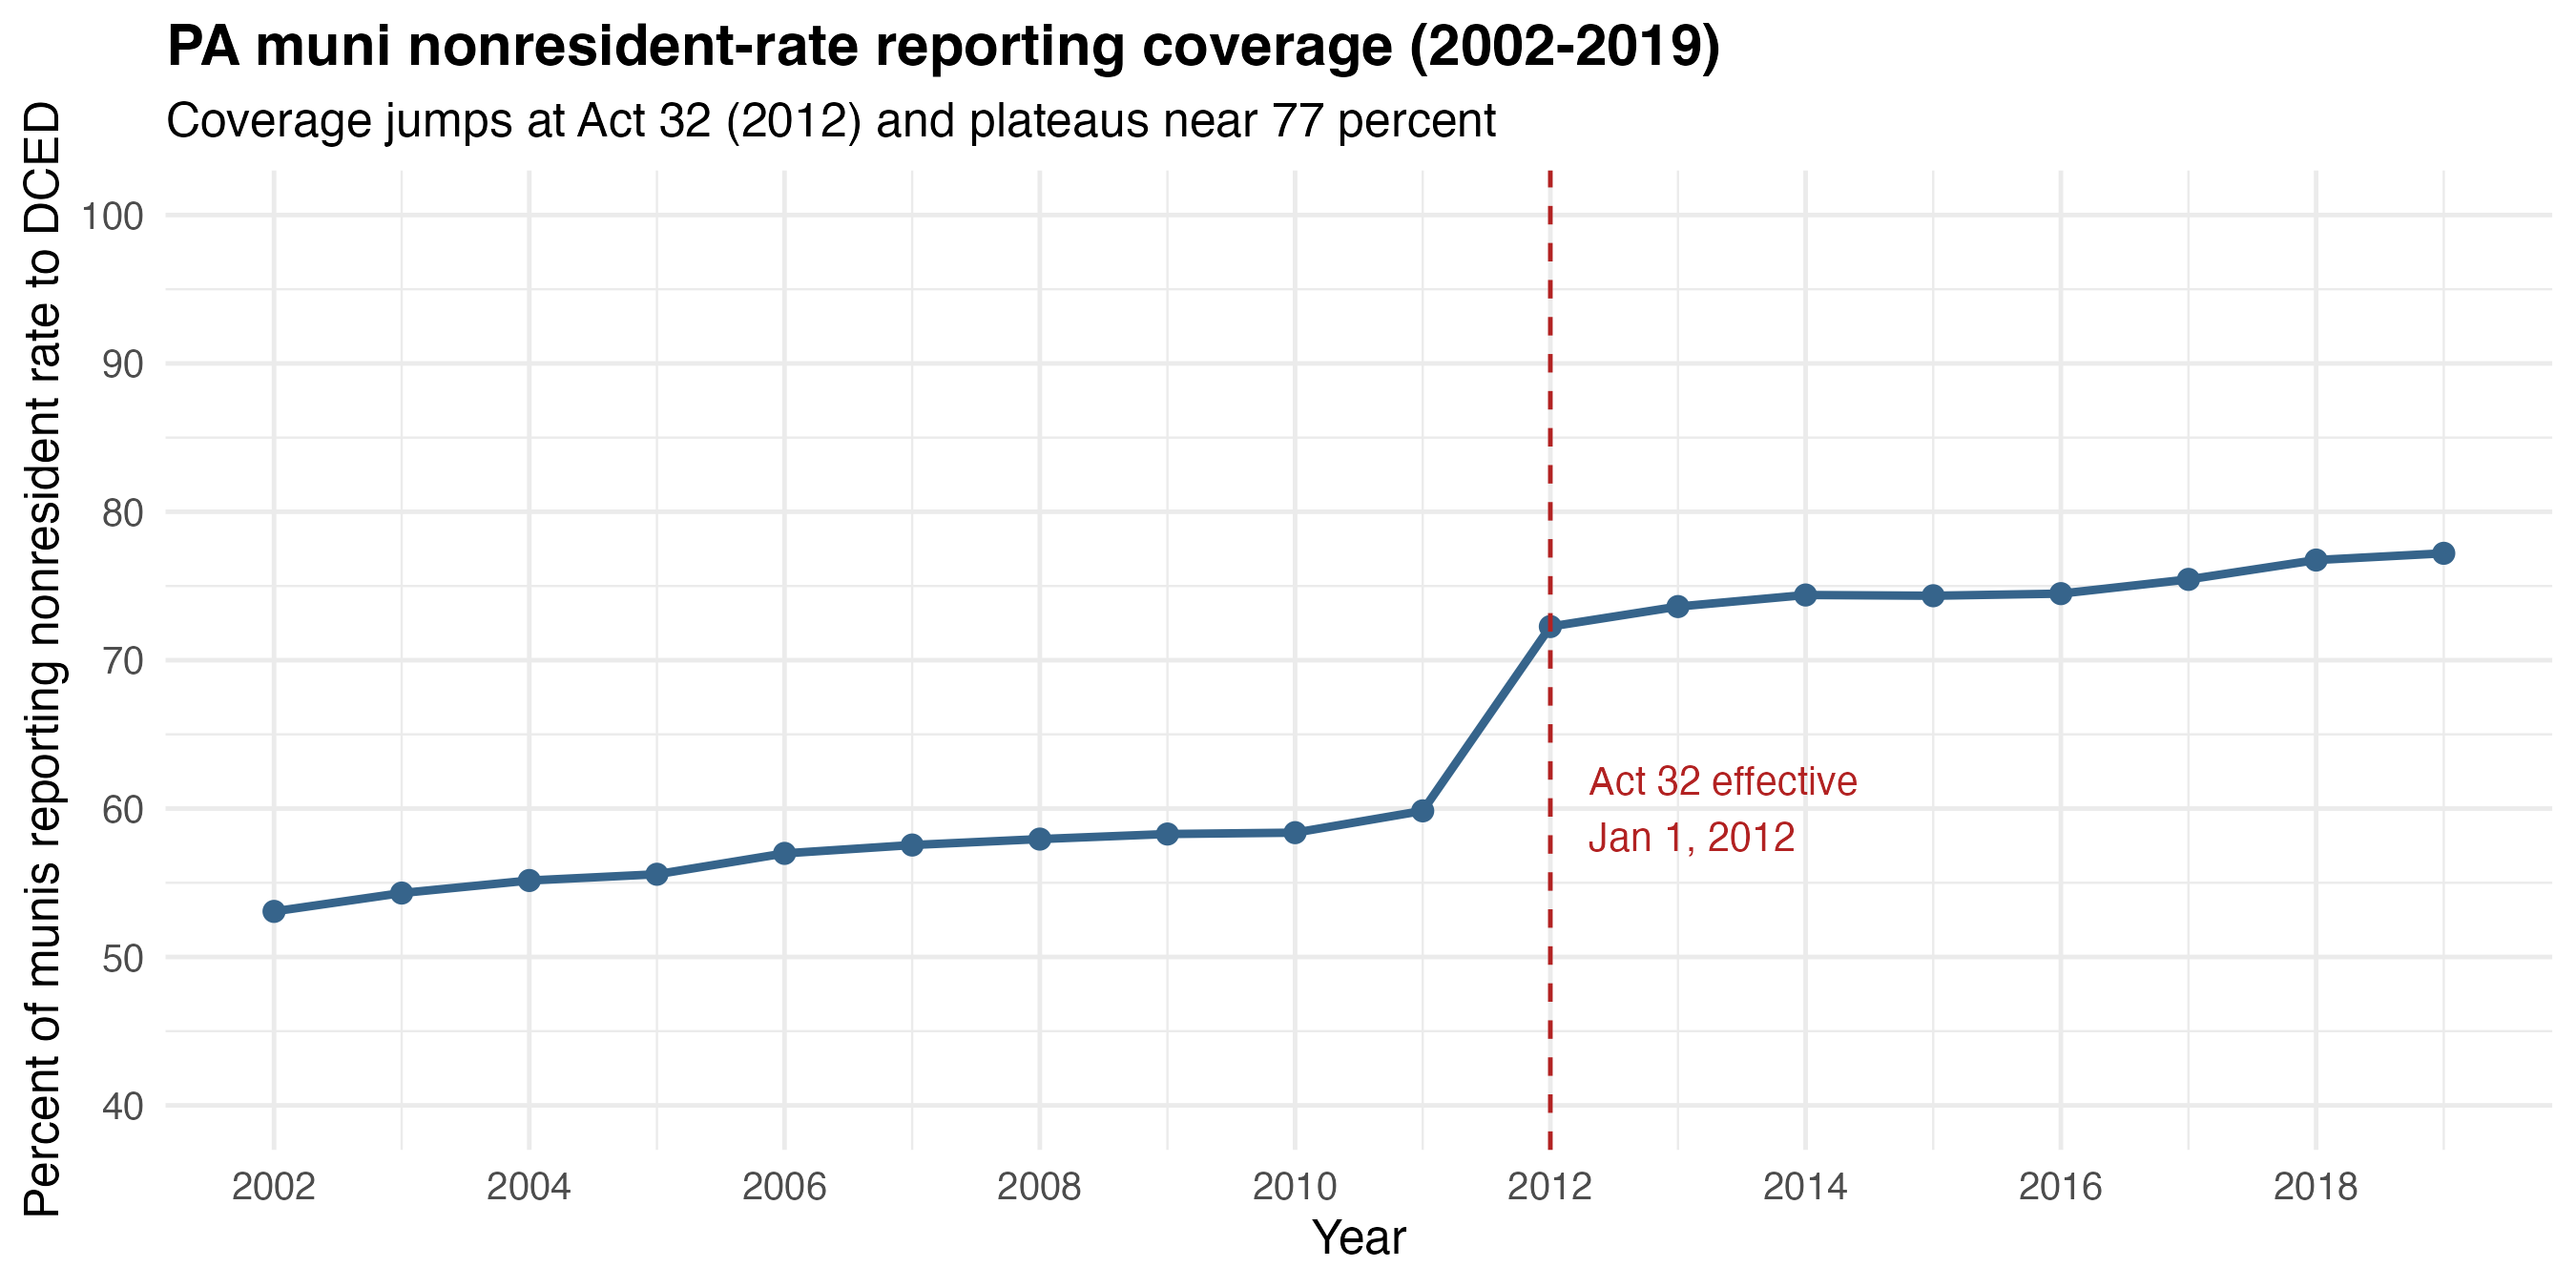
\includegraphics[width=0.85\textwidth]{../figures/nonres_coverage.png}
    \caption{Share of PA municipalities reporting a work
    rate to DCED, by year. The break at 2012 reflects the Act 32
    requirement that employers withhold at the higher of the home
    resident and work rates.}
    \label{fig:act32_cdf}
\end{figure}

School districts in Pennsylvania also levy an EIT under Act 511
\citep{paAct511_1965}, typically at 0.5\% (the other half of the
standard 1\% cap). Act 1 of 2006 \citep{paAct1_2006} (the Taxpayer
Relief Act) additionally authorized
school districts to exceed the 0.5\% cap specifically to fund
property tax relief. I find that the correlation between the municipal and school-district resident rates is only weakly negative of $-0.12$ indicating the two taxing jurisdictions move on relatively separate schedules. Since every census block sits in both a municipality
and a school district, workers face two overlapping EIT rates
that can change independently, providing a natural decomposition
of the residential sorting response into municipal and school
district components.

\subsection{Pennsylvania Property Tax}
\label{subsec:proptax-inst}

The same municipalities, together with their counties, levy a real-estate
property tax. Each taxing body sets a millage rate applied to the
\emph{assessed} value of a parcel; the assessed value is a county-set
fraction of market value, and the State Tax Equalization Board (STEB)
certifies that fraction---the common-level ratio (CLR)---for each county
annually. The municipal and county millage are reported in the same DCED
tax register that reports the EIT, so a municipality-by-year panel of
both is directly available; the school-district real-estate millage is
also reported but the school district is not used as an estimating unit
here. Two institutional features shape the analysis. Pennsylvania
reassesses infrequently and irregularly---many counties had not reassessed
in decades during the sample, and only $24$ of $67$ reassessed at all over
2002--2019---so the CLR drifts downward between reassessments as market
values outpace stale assessments. And the Act~1 anti-windfall provisions
require that millage be rolled back to revenue-neutrality at a
reassessment, with any real increase requiring a separate, capped vote.
These features mean the statutory millage and the effective burden it
implies can diverge, which is why the analysis works with the effective
rate (millage $\times$ CLR) and its policy-driven component rather than
raw millage (Section~\ref{subsec:proptax-theory}). Unlike the EIT, the
property tax falls on the dwelling rather than the worker, the
distinction the comparison turns on.

%==========================================================
\section{Conceptual Framework: Binding Decomposition}
\label{sec:theory}
%==========================================================

The piecewise tax allocation in Equation~(\ref{eq:piecewise}) is the causal
identification backbone of my empirical design. A worker's bill is
$T = \max(\tau^{\text{home}}, \tau^{\text{work,muni}})$. A rate change
only moves the bill when its side of the max binds. The
implied change in the worker's bill from a single rate event is
\[
  \Delta T \;=\; \max(\tau^{\text{home}}_{\text{post}}, \tau^{\text{work,muni}})
              - \max(\tau^{\text{home}}_{\text{pre}},  \tau^{\text{work,muni}}),
\]
which depends jointly on the direction of the rate change and on
which side of the max is binding pre- and post-event. This tax difference from pre and post rate changes can
produce a strong sorting response, a moderate response, or no
response at all depending on the binding transition.

\subsection{Six Cells per Rate-Setter}
\label{subsec:cells}

Two definitions structure the decomposition. First, the piecewise
rule $T = \max(\tau^{\text{home}}, \tau^{\text{work,muni}})$ has two
sides: the home side
$\tau^{\text{home}} = \tau^{\text{res,muni}} + \tau^{\text{SD}}$,
set at the worker's residence, and the work side
$\tau^{\text{work,muni}}$, the work rate set by the worker's workplace municipality.
Whichever side is larger is the binding side and determines
the bill. Second, three rate-setters adjust statutory rates
independently across municipality-years: the municipality resident
rate $\tau^{\text{res,muni}}$, the school-district rate
$\tau^{\text{SD}}$, and the municipality work rate
$\tau^{\text{work,muni}}$. The decomposition is built one rate-setter
at a time.

For each rate-setter $\tau$, a cell classifies a municipality
by the direction of its first rate event in $\tau$ (Increase or
Decrease) and then the binding transition of its home stack
across that event: stayed-binding, flipped, or stayed-non-binding.
The cross gives six cells plus a seventh never-changed control pool,
of which only the three Increase cells and the NC control are used in
this paper (Table~\ref{tab:cells}). Each municipality therefore carries three
cell labels (one for each of $\tau^{\text{res,muni}}$,
$\tau^{\text{SD}}$, and $\tau^{\text{work,muni}}$) and the binding
state for each is determined by where its home stack sits relative
to its work rate at the time of that event.

\begin{table}[H]
\centering
\small
\begin{tabular}{lcccl}
\toprule
Cell & Direction & Pre-binding? & Post-binding? & Bill effect \\
\midrule
Inc-bind         & $\uparrow$  & yes & yes & rises by full $\Delta\tau$ \\
Inc-becomes      & $\uparrow$  & no  & yes & rises by part of $\Delta\tau$ \\
Inc-nobind       & $\uparrow$  & no  & no  & no change (placebo) \\
NC               & none & --- & --- & control pool \\
\bottomrule
\end{tabular}
\caption{Binding cells per rate-setter on the increase side. For Inc-becomes the bill rises only by the portion of $\Delta\tau$ above the work rate. Three mirror decrease cells exist by construction but are not estimated in this paper because the decrease cohort is too thin to support causal inference ($5$ Dec-bind, $3$ Dec-becomes-non, $11$ Dec-nobind) and the realized-dose pre-trend rejects parallel trends on every Dec outcome.}
\label{tab:cells}
\end{table}

The cell labels describe the state of the home stack at the
rate event and not necessarily which rate-setter is caused the cell to be that state.
The home stack $\tau^{\text{home}} = \tau^{\text{res,muni}} + \tau^{\text{SD}}$ is
additive in its two home-side components where either component can put
the stack above or below the work floor. A municipality
therefore carries two independent cell labels, one for each
rate-setter (municipality and school district), and the two are not mutually exclusive such as when a muni
classified as Inc-bind on the muni side may be Inc-becomes on the
SD side (or any other combination). The interaction terms in the
estimating equation (Section~\ref{sec:strategy}) separate the
per-pp effect of a muni-rate change from the per-pp effect of an
SD-rate change, each conditional on its own cell label.

What the labels imply for an individual worker depends on where
that worker is employed. Under Act~32 the employer withholds at
$\max(\tau^{\text{home}}, \tau^{\text{work,muni}})$, where
$\tau^{\text{work,muni}}$ is the work rate of the
worker's workplace \citep{paAct32_2008, bagchiEffectsIntroducingWithholding2022}. For a worker who lives and works in
municipality $i$ the workplace rate is exactly $i$'s
own $\tau^{\text{work,muni}}_i$, which is the comparison floor the cell
classification uses. For a resident of $i$ who works in a different
municipality $j$, the relevant floor is $\tau^{\text{work,muni}}_j$,
which the LODES origin--destination data does not let us recover at
the worker level and therefore the label using $i$'s own
work rate is an aggregate proxy that is reasonable on
average across Pennsylvania's local commute shed but not verifiable
individually. This distinction motivates the outcome ordering in
Section~\ref{sec:results}: the count of workers who live and work
in their own municipality, $\log(\text{live-and-work})$, is the
cleanest binding-rule test because the classification matches each
worker's actual workplace and the model directly estimates the response of those who face either $\tau^{\text{home}}$ or $\tau^{\text{work,muni}}$. The other count outcomes are noisier tests: $\log(\text{total jobs})$ and the share of workers living in their own municipality both fold in in-commuters, and $\log(\text{in-commuters})$
does not test the muni resident-rate binding rule at all because
in-commuters' bills do not depend on the resident rate of the
municipality where they work.

The fundamental testable prediction is an
ordered ranking of cell magnitudes where Inc-bind effects exceed
Inc-becomes effects, which in turn exceed Inc-nobind effects, with
the last close to zero and serving as the
within-design placebo. A tax salience argument would state that workers in the Inc-becomes cell
experience a discrete switch from paying zero home-side tax to
paying a positive amount, which should trigger a large behavioral response. The
central empirical comparison of the paper is between Inc-bind and
Inc-nobind where if statutory rates matter mechanically through tax
liability, the residential response should appear in Inc-bind and
not in Inc-nobind. If Inc-nobind moves, the mechanism
interpretation fails and the response is something other than the
binding rule because Inc-nobind events do not change the worker's
bill. This makes the design self-falsifying in a way that a
conventional pooled-Increase specification is not. In the pooled
specification, every increase is a treated event, while here the
institutional rule predicts that only a subset of statutory
increases should generate a response.

\subsection{The Property Tax: A Continuous Treatment Without a Placebo}
\label{subsec:proptax-theory}

The property tax has no piecewise structure and therefore no binding
decomposition. Every increase in the rate raises the bill of every
resident owner directly (and renters through capitalized rents), so
there is no non-binding cell and no within-design placebo. The treatment
is the \emph{effective} property-tax rate on market value,
\[
  \tau^{P}_{it} \;=\; \big(\text{mills}^{\text{muni}}_{it}
  + \text{mills}^{\text{county}}_{it}\big)\big/1000 \;\times\; \text{CLR}_{c(i),t},
\]
where the common-level ratio $\text{CLR}$ (assessed value over market
value, certified annually by the State Tax Equalization Board for each
county $c$) converts statutory mills, levied on assessed value, into a
rate on market value that is comparable across counties with different
assessment practices. Two features of $\tau^{P}$ require care. The
CLR drifts mechanically between countywide reassessments as market values
rise and assessments lag, and that drift is correlated with local
house-price growth---itself a driver of location choice---so the raw
effective rate is not a clean policy treatment. And Pennsylvania law
makes reassessments revenue-neutral (millage is rolled back as the base
jumps), so a statutory millage \emph{cut} at reassessment need not lower
the burden at all. I therefore use the policy-driven component: the
cumulative \emph{discretionary} millage change valued at the
municipality's baseline assessment ratio, where the reassessment-year
increment is measured as the deviation from the revenue-neutral rollback
(zero for a pure rollback, positive only when the rate is set above
revenue-neutral). This strips the endogenous drift and the mechanical
rebasing from the treatment.

The cost of this cleaner treatment is weaker identification than the
EIT. Property millage changes almost every year (the school-district
component moves under the Act~1 index, and municipalities and counties
adjust frequently), so there is no never-treated control pool;
identification comes from variation in the \emph{magnitude} of the
cumulative policy dose across municipalities, not from a clean
treated-versus-untreated contrast. And, lacking a binding rule, the
property tax has no placebo cell to fall back on. Its only
identification check is the realized-dose pre-trend
(Section~\ref{sec:strategy}). I state this asymmetry plainly: the EIT
result is validated by both a clean pre-trend and a within-design
placebo; the property-tax result rests on the pre-trend alone, and I
report what that single check can and cannot support.

%==========================================================
\section{Data}
\label{sec:data}
%==========================================================

\subsection{Data Sources}
\label{subsec:sources}
\label{subsec:sample}
\label{subsec:pipeline}

The analysis merges the LEHD  residence--workplace dataset and the  Pennsylvania EIT rate records to create a panel of rate changes and workforce data over space and time. The two datasets do not share common identifiers, and was bridged using TIGER~2020 block geometry, which
nests blocks within county subdivision code (cousubs). A
municipality-name crosswalk maps each DCED municipality ID to its
corresponding COUSUBFP code, matching $2{,}496$ of $2{,}505$ PA municipalities
($99.6\%$). The remaining $9$ are small boroughs that have either dissolved or
merged during 2002--2019 and are dropped from the analysis.

The residence--workplace data come from LEHD LODES Version~8,
2002--2019 \citep{lehdLODES}. The Census Bureau applies
synthetic noise infusion at the block level to protect respondent
confidentiality and is calibrated so that aggregation to tract and larger
geographies approximates ground truth
\citep{grahamDESIGNCOMPARISONLODES}. The sample period of 2002--2019
reflects LODES coverage beginning in 2002 and
2020--2023 to not include disruptions in the data resulting from the COVID Pandemic.

Municipal and school-district EIT rates come from the Pennsylvania
Department of Community and Economic Development (DCED) MunStats
portal \citep{padcedMunStats}, scraped annually. In some DCED reports, the flat-dollar Local Services Tax is filled in the same field
as the EIT in some years, so rates above $5\%$ are treated as
data-entry errors and dropped except for Home Rule cities and Philadelphia.

Municipal fiscal controls come from the PA DCED Statewide Municipal
Annual Financial Report database \citep{padcedAFR}. School-district
fiscal controls come from the Census Annual Survey of School System
Finances (F-33) \citep{censusF33}; the NCES \texttt{LEAID}-to-DCED
SD ID crosswalk covers all $500$ school districts. All fiscal
controls are share-based and time-varying. Municipality regressions
use six DCED AFR shares: three expenditure shares
(police-services, streets, debt-service) and three revenue shares
(EIT-revenue, real-estate-tax, intergovernmental-revenue).
LODES blocks are aggregated to muni for analysis.

The municipality--SD assignment uses the modal SD ID per muni in
the DCED rate panel ($97.6\%$ of municipalities are single-SD), so
each muni-year carries a single $\tau^{\text{SD}}$ co-treatment.
Municipality regressions
further impose a
minimum employment threshold of $50$ total jobs, which protects the
share-based outcomes from mechanical noise (a single worker moving
changes a share by $1/N$, so at $N=10$ a one-worker move dominates
the per-pp coefficient) and matches the LODES synthetic-noise
calibration that is validated at tract scale and above
\citep{grahamDESIGNCOMPARISONLODES}. The threshold drops $185$ of
$2{,}559$ municipalities ($7.2\%$), almost all sparsely populated
NC-pool townships; the treated cohort is essentially unaffected.

For the property-tax leg, municipal and county real-estate millage come
from the same DCED MunStats register, scraped annually
\citep{padcedMunStats}; the county tax register reports general-purpose
and total millage for all $66$ assessing counties (Philadelphia is a
consolidated city--county). County common-level ratios come from the
Pennsylvania Department of Revenue's historical CLR factor series, in
which the published factor is the reciprocal of the CLR; its
assessment-base-change footnotes also date each countywide reassessment,
which I use to flag reassessment years. The effective property-tax rate
combines municipal and county millage with the county CLR; across
municipality-years its median is about $2.1\%$ of market value (with the
school district excluded as an estimating unit). To put the income and
property taxes on a common dollar basis I use each municipality's own
median household income (ACS table B19013) and median owner-occupied
home value (B25077) from the American Community Survey five-year files,
which cover county subdivisions from the 2005--2009 release onward;
coverage is $99.7\%$ of municipalities, missing cells are filled with the
county median (flagged), and pre-2009 panel years hold the 2009 value
(flagged). The cross-municipality home-to-income ratio has a median of
$2.6$ (10th--90th percentile $1.8$--$3.5$), the spread that drives the
sensitivity band on the per-dollar comparison.

\subsection{Descriptive Statistics}
\label{subsec:descriptive}

This section presents the summary statistics at the municipality
level. The primary outcome variables are resident-worker counts,
workplace counts, in-commuter flows, and the live-and-work share.
Fiscal outcomes used as control variables (log EIT revenue, log
total tax revenue, log total revenue, log police expenditure) are
reported in Appendix~\ref{app:robustness}.

Table~\ref{tab:summary_muni} summarizes the estimation panel.

% (block summary removed; muni is the only estimating unit)
% \begin{table}[H]
  \centering
  \caption{Block-year summary statistics (2002--2019)}
  \label{tab:summary_block}
  \small
  \resizebox{\textwidth}{!}{
  \begin{tabular}{lrrrrrrrr}
    \toprule
    Variable & N & Mean & SD & p25 & p50 & p75 & Min & Max \\
    \midrule
    Home count (workers living) & 5,030,958 & 18.822 & 31.677 & 4.000 & 10.000 & 22.000 & 0.000 & 1572.000 \\
    $\log$ home count & 4,795,213 & 2.293 & 1.198 & 1.386 & 2.398 & 3.135 & 0.000 & 7.360 \\
    Work count (jobs in block) & 5,030,958 & 18.826 & 138.957 & 0.000 & 0.000 & 4.000 & 0.000 & 20945.000 \\
    $\log$ work count & 1,894,432 & 2.256 & 1.663 & 1.099 & 2.079 & 3.367 & 0.000 & 9.950 \\
    Share live-and-work in muni & 4,795,213 & 0.154 & 0.222 & 0.000 & 0.067 & 0.203 & 0.000 & 1.000 \\
    Share work outside muni & 4,795,213 & 0.846 & 0.222 & 0.797 & 0.933 & 1.000 & 0.000 & 1.000 \\
    Resident rate $\tau^{M}$ (\%) & 4,782,928 & 0.762 & 0.799 & 0.500 & 0.500 & 0.500 & 0.000 & 4.331 \\
    SD rate $\tau^{SD}$ (\%) & 4,782,928 & 0.607 & 0.376 & 0.500 & 0.500 & 0.500 & 0.000 & 2.050 \\
    Nonresident rate $\tau^{nr,M}$ (\%) & 4,181,214 & 1.063 & 0.657 & 1.000 & 1.000 & 1.000 & 0.000 & 3.820 \\
    Blocks per muni & 2,561 & 120.922 & 384.585 & 41.000 & 73.000 & 132.000 & 1.000 & 16550.000 \\
    \bottomrule
  \end{tabular}
  }
  \vspace{0.3em}
  \begin{minipage}{0.95\textwidth}
    \footnotesize \textit{Notes:} Block-year level; one observation per (census block, year). Panel covers 309,680 blocks in 2,561 municipalities.
  \end{minipage}
\end{table}


\begin{table}[H]
  \centering
  \caption{Muni-year summary statistics (2002--2019)}
  \label{tab:summary_muni}
  \small
  \resizebox{\textwidth}{!}{
  \begin{tabular}{lrrrrr}
    \toprule
    Variable & N & Mean & SD & Min & Max \\
    \midrule
    Resident rate $\tau^{M}$ (\%) & 43,374 & 0.525 & 0.163 & 0.000 & 4.331 \\
    Nonresident rate $\tau^{nr,M}$ (\%) & 34,080 & 0.883 & 0.237 & 0.000 & 3.820 \\
    SD rate $\tau^{SD}$ (\%) & 43,374 & 0.622 & 0.289 & 0.000 & 2.050 \\
    Home stack $\tau^{M}+\tau^{SD}$ (\%) & 43,374 & 1.147 & 0.316 & 0.000 & 4.331 \\
    $\log$ live-and-work & 40,748 & 3.638 & 2.011 & 0.000 & 12.877 \\
    $\log$ total jobs & 45,291 & 5.819 & 2.006 & 0.000 & 13.353 \\
    Share live-and-work in muni & 45,291 & 0.095 & 0.081 & 0.000 & 1.000 \\
    \bottomrule
  \end{tabular}
  }
  \vspace{0.3em}
  \begin{minipage}{0.95\textwidth}
    \footnotesize \textit{Notes:} Muni-year level; one observation per (municipality, year). Rates in percentage points. $\tau^{nr,M}$ has reporting gaps before Act 32; the $N$ for that row is smaller than the full panel.
  \end{minipage}
\end{table}


Table \ref{tab:summary_muni} presents the municipality level summary statistics. Table \ref{tab:summary_muni} shows that there are roughly $43{,}374$ muni-year observations, and the resident rate is tightly clustered
near the Act~511 default at $\bar{\tau}^{M}=0.53\%$ and a standard deviation of $0.16$pp. There is a long right tail indicated by the max rate of $4.33\%$ concentrated in Philadelphia and
a handful of Home-Rule and Act~47 distressed cities. The
work rate has $34{,}080$ observation, about $9{,}300$ fewer
observations than the resident rate, due to DCED's lack of coverage for the work-rate field being incomplete before Act~32 mandated
reporting. The SD rate has nearly twice the
muni-rate dispersion (SD $0.29$pp vs.\ $0.16$pp) and maxes at $2.05\%$, potentially making the school-district
rate-setter a larger statistical lever. The home stack averages
$1.15\%$, above the $1\%$ Act~511 cap, because Act~1 SD increases
and Home-Rule muni rates push the upper level past the ceiling.
Only $9.5\%$ of muni jobs are
held by residents of the same muni showing that residential sorting operates
on a thin within-muni margin.



% \begin{table}[H]
  \centering
  \caption{School-district-year summary statistics (2002--2019)}
  \label{tab:summary_sd}
  \small
  \resizebox{\textwidth}{!}{
  \begin{tabular}{lrrrrrrrr}
    \toprule
    Variable & N & Mean & SD & p25 & p50 & p75 & Min & Max \\
    \midrule
    SD rate $\tau^{SD}$ (\%) & 49,226 & 0.610 & 0.278 & 0.500 & 0.500 & 0.500 & 0.000 & 2.050 \\
    Resident rate $\tau^{M}$ (\%) (muni-year) & 49,226 & 0.523 & 0.162 & 0.500 & 0.500 & 0.500 & 0.000 & 4.564 \\
    Nonres rate $\tau^{nr,M}$ (\%) (muni-year) & 38,536 & 0.881 & 0.237 & 1.000 & 1.000 & 1.000 & 0.000 & 3.967 \\
    share\_state\_rev\_sd & 9,278 & 0.416 & 0.166 & 0.279 & 0.414 & 0.555 & 0.000 & 0.821 \\
    share\_local\_rev\_sd & 9,278 & 0.536 & 0.186 & 0.376 & 0.536 & 0.691 & 0.103 & 1.000 \\
    share\_federal\_rev\_sd & 9,278 & 0.048 & 0.033 & 0.024 & 0.040 & 0.062 & 0.000 & 0.247 \\
    share\_property\_tax\_sd & 9,278 & 0.420 & 0.176 & 0.270 & 0.407 & 0.562 & 0.000 & 0.853 \\
    share\_instructional\_sd & 9,278 & 0.522 & 0.070 & 0.492 & 0.536 & 0.567 & 0.000 & 1.000 \\
    share\_support\_sd & 9,278 & 0.279 & 0.039 & 0.259 & 0.284 & 0.305 & 0.000 & 0.438 \\
    \bottomrule
  \end{tabular}
  }
  \vspace{0.3em}
  \begin{minipage}{0.95\textwidth}
    \footnotesize \textit{Notes:} SD-year level. F-33 share controls are constructed from Census F-33 revenue/expenditure totals.
  \end{minipage}
\end{table}
  % (SD summary table removed; see paper scope)

\begin{table}[H]
  \centering
  \caption{Cell counts: muni resident-rate side, 2002--2019}
  \label{tab:cell_counts_summary}
  \small
  \begin{tabular}{lrrrr}
    \toprule
    Cell & Munis & Muni-years & Mean dose (pp) & Extreme dose (pp) \\
    \midrule
    Never-changers & 1,730 & 31,132 & 0.000 & 0.000 \\
    Inc-bind & 24 & 432 & 0.168 & 0.850 \\
    Inc-becomes & 43 & 774 & 0.246 & 1.250 \\
    Inc-nobind & 20 & 360 & 0.294 & 0.650 \\
    Dec-bind & 4 & 72 & -0.138 & -0.500 \\
    Dec-becomes-non & 3 & 54 & -0.278 & -0.500 \\
    Dec-nobind & 11 & 198 & -0.380 & -1.000 \\
    \bottomrule
  \end{tabular}
  \vspace{0.3em}
  \begin{minipage}{0.95\textwidth}
    \footnotesize \textit{Notes:} Cells classify each muni's first resident-rate event by direction (Inc/Dec) and the binding-state transition relative to the muni's nonresident rate. NC is the never-changed control pool. Dose is the cumulative $\Delta\tau$ within the 5-year event window. The Extreme dose column reports the max cumulative dose for Inc cells and the min (most negative) cumulative dose for Dec cells, since cell assignment is determined by the first event but subsequent reversals can pull the signed cumulative path back across zero.
  \end{minipage}
\end{table}


Table~\ref{tab:cell_counts_summary} reports the cell
assignments on the muni resident-rate side. Of roughly $2{,}560$
municipalities, after dropping those that decrease or flip-flop any of
their three rates, $1{,}687$ never-changers form the NC control pool and
only $77$ enter one of the three increase cells, split as $24$ Inc-bind,
$39$ Inc-becomes, and $14$ Inc-nobind.
Inc-becomes shows a larger average
dose than Inc-bind, indicating that crossing the binding threshold typically
requires a bigger statutory move than slowly inching up an already-binding
rate.

Figure~\ref{fig:rate_changes_by_year} reports the timing of
municipal resident-rate changes across the panel. Increases jumped in the early 2000s, from 2002 to 2009 and taper off after. Most of the identifying variation in my models predates Act 32, highlighting the significant effects found are on smaller increases and further warranting a pre-post 2012 decomposition.

\begin{figure}[H]
    \centering
    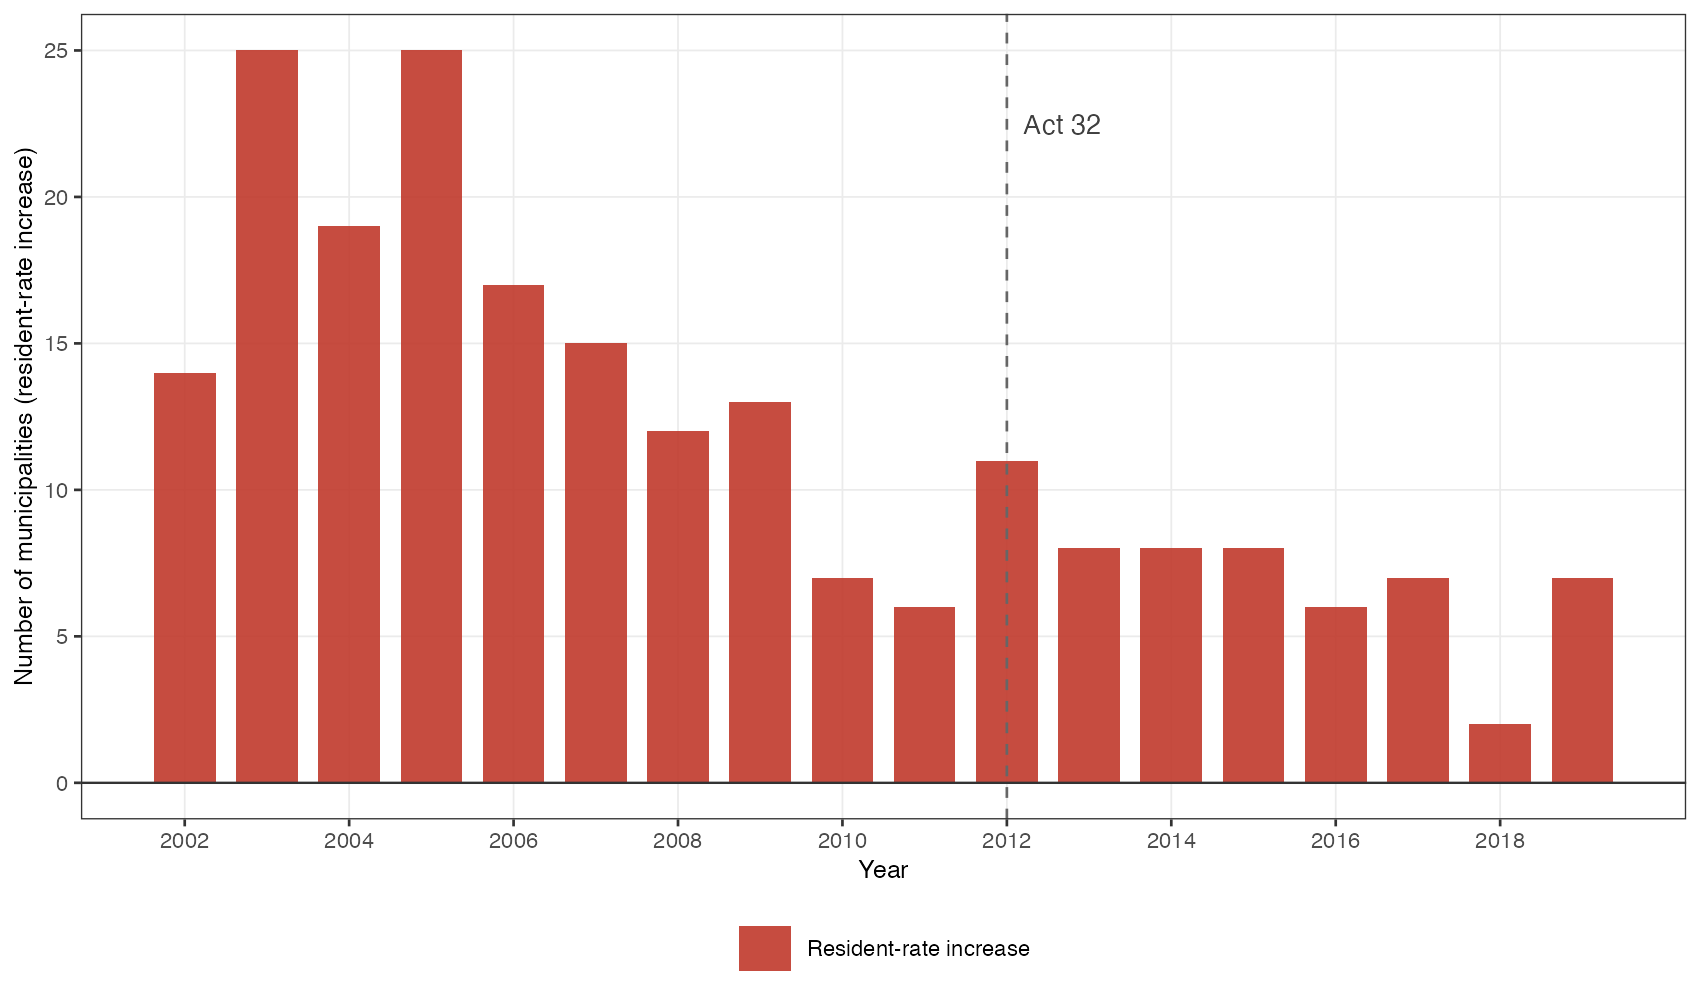
\includegraphics[width=0.95\textwidth]{../figures/rate_changes_by_year.png}
    \caption{Number of PA municipalities changing their resident
    rate, by year. Increases shown above zero; decreases shown below.
    Dashed line: 2012, when Act 32 consolidated withholding.}
    \label{fig:rate_changes_by_year}
\end{figure}

Lastly, figure~\ref{fig:pa_map} shows the spatial distribution of the rate changers in my sample. Most rate changers occur along the east coast, but some are also scattered within the interior of the state. This spatial distribution highlights the value of future work to understand the effects when two neighboring municipalities raise or lower rates across time.

% --- Treatment Geography Map ---
\begin{figure}[H]
    \centering
    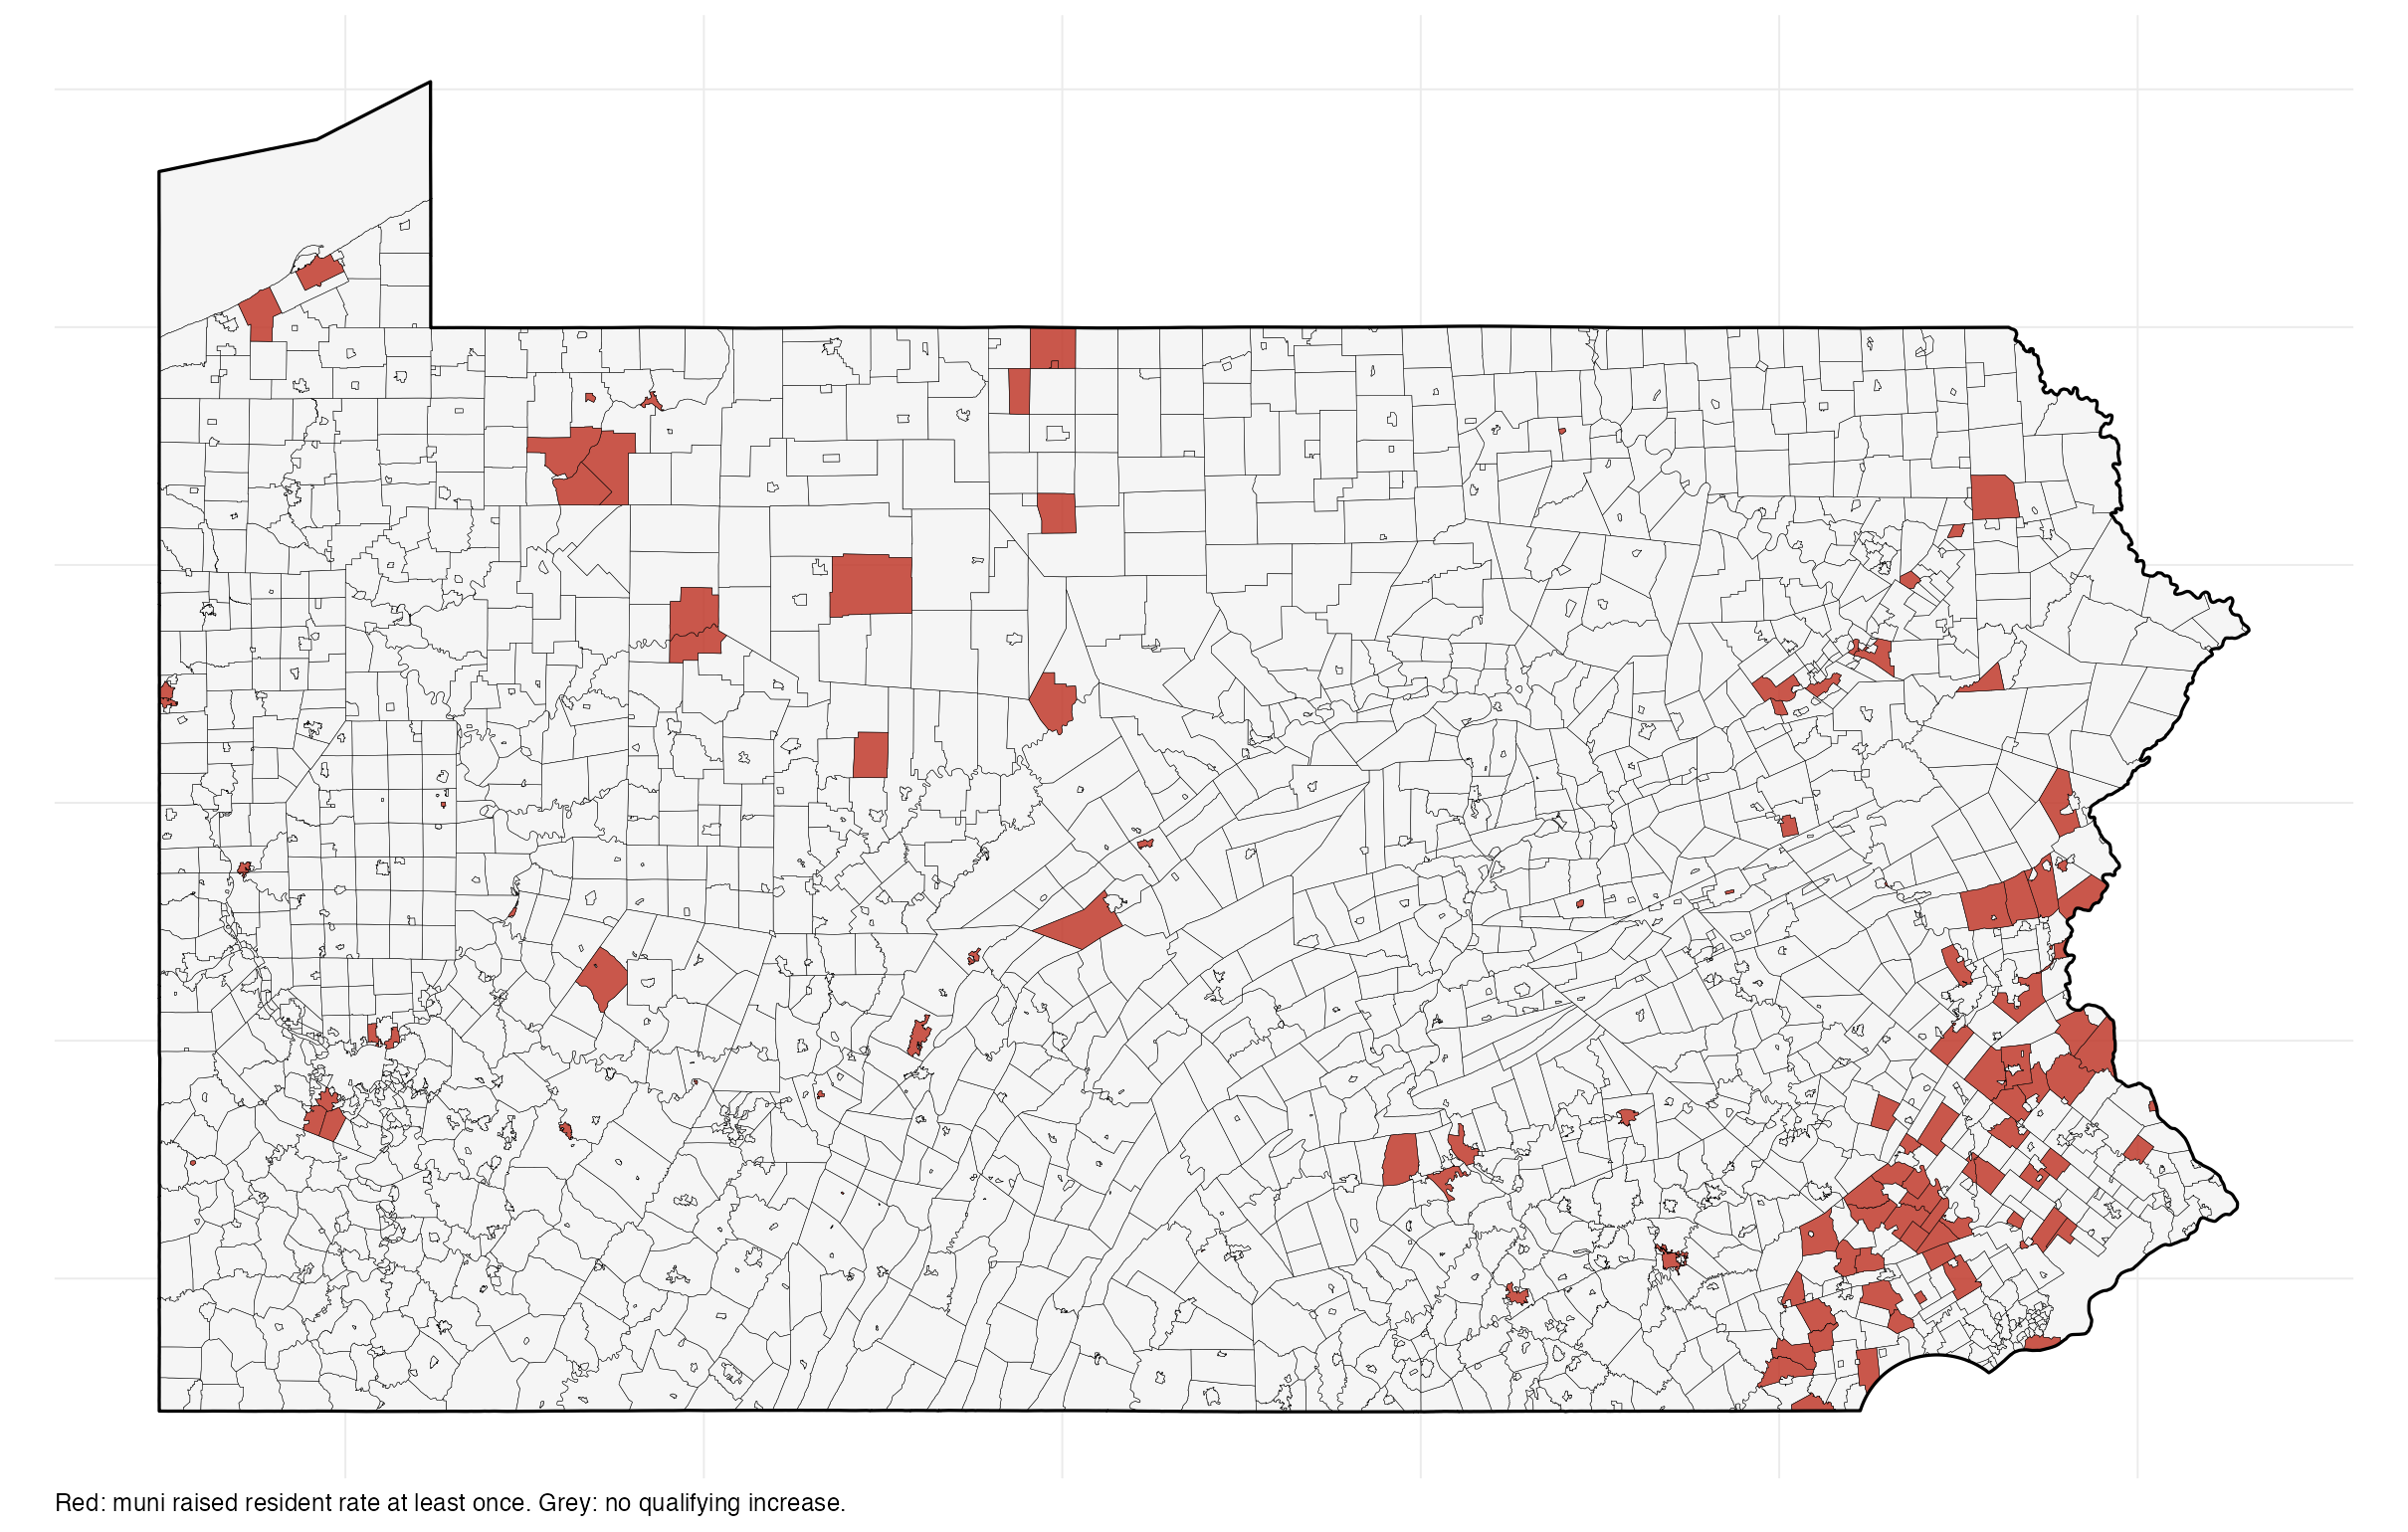
\includegraphics[width=0.85\textwidth]{../figures/pa_map.png}
    \caption{Pennsylvania EIT rate changes, 2000--2019. Red =
    increased; blue = decreased; purple = both; grey = no change.}
    \label{fig:pa_map}
\end{figure}

%==========================================================
\section{Empirical Strategy}
\label{sec:strategy}
%==========================================================

I estimate two specifications using a continuous stacked
difference-in-differences design. First, I run a pooled-Increase
aggregate (\S\ref{subsec:pooled-spec}) that collapses all
rate-increase events at each rate-setter into a single only-increase
group. Second, I estimate a binding
decomposition (\S\ref{subsec:stacked-continuous}) on the three
Increase cells defined in
Section~\ref{sec:theory}, isolating the rate changes that move the
worker's bill from those that do not. Both specifications are
estimated at the municipality-year level. Decrease cells are not estimated: the cohort is
thin ($5$ Dec-bind, $3$ Dec-becomes-non, $11$ Dec-nobind) and the
realized-dose pre-trend rejects parallel trends on every Dec outcome
(Wald $p<0.001$), so the Dec coefficients cannot be interpreted as
causal. It is important to note that a theoretical case for symmetric responses to
rate cuts and rate hikes is important but most likely weak. First, moving costs are
sunk, so the effect of rate cuts may be less salient to incumbent residents
than rate hikes. Pre-trends are tested
separately by a realized-dose Sun--Abraham event study
(\S\ref{subsec:pretrend-diagnostics}). This section focuses on
estimating equations, identification, and diagnostics.


\subsection{Pooled Aggregate Specification}
\label{subsec:pooled-spec}

In this section I report an aggregate specification that pools the
treated Increase cells per rate-setter into a single directional group
$\text{Inc}$ (any rate increase), with never-changers (NC) as the omitted reference. Decrease cells
are excluded because the cohort is
thin ($5$ Dec-bind, $3$ Dec-becomes-non, $11$ Dec-nobind) and the
realized-dose pre-trend rejects parallel trends on every Dec outcome
(Wald $p<0.001$). The pooled
regression answers: what is the average per-percentage-point (pp)
effect of a rate hike on residents, ignoring whether or not the
hike binds? The binding decomposition that follows in
Equation~(\ref{eq:headline}) then explains how the binding mechanism drives the pooled coefficient.

For each unit-time observation $(i, t)$ on the stacked panel, the
per-pp pooled regression is

\begin{equation}
\begin{split}
Y_{\tilde i \tilde t} \;=\; \alpha_{\tilde i} \;+\; \gamma_{\tilde t}
&+ \beta^{M}_{\text{Inc}}\;\Delta\tau^{M}_{it}\,\mathbf{1}\!\left\{d^{M}_{i} = \text{Inc}\right\} \\
&+ \beta^{SD}_{\text{Inc}}\;\Delta\tau^{SD}_{it}\,\mathbf{1}\!\left\{d^{SD}_{i} = \text{Inc}\right\} \\
&+ \mathbf{X}'_{it}\boldsymbol{\phi}
\;+\; \varepsilon_{\tilde i \tilde t}.
\end{split}
\label{eq:pooled}
\end{equation}

The dependent variable $Y_{\tilde i \tilde t}$ is the outcome of
interest. At the municipality level the
outcomes are the logs of live-and-work workers (residents employed
in their own municipality), in-commuters, log total jobs, and the
share of workers living in their own municipality. The unit $i$ is a municipality and $t$ a calendar year. The subscripts $\tilde i = (i, c)$ and
$\tilde t = (t, c)$ are the unit-by-stack and year-by-stack
groupings where each treated unit $i$ appears in exactly one
sub-experiment (its first-event cohort $c$), while each NC unit
appears in every cohort it overlaps. Cohort $c$ is defined as the first year that the rate-setter changed $\tau$. The fixed effects
$\alpha_{\tilde i}$ and $\gamma_{\tilde t}$ are for each unit and cohort pair. The directional grouping
$d^{s}_{i} \in \{\text{NC}, \text{Inc}\}$ classifies
unit $i$'s rate trajectory on rate-setter $s \in \{M, SD\}$, with
NC the omitted reference as they are the control group. The
dose $\Delta\tau^{s}_{it} = \tau^{s}_{it} - \tau^{s}_{i, c-1}$ is
the cumulative change in the rate from the pre-event baseline
($c-1$, one year before the first event) to year $t$, measured in
percentage points; it is zero in pre-event years and for NC units,
and accumulates with subsequent rate changes within $i$. The control vector
$\mathbf{X}_{it}$ holds the six municipality fiscal share controls
(police-services, streets, debt-service, EIT-revenue,
real-estate-tax, intergovernmental-revenue).
$\boldsymbol{\phi}$ is the
coefficient vector on these controls and $\varepsilon_{\tilde i \tilde t}$
is the error term.

\subsection{Binding Decomposition: Stacked Continuous DiD}
\label{subsec:stacked-continuous}

The binding decomposition is the main estimator of the paper. It
replaces the two-level direction grouping $d^s_i$ from
Equation~\ref{eq:pooled} with a multilevel cell
$\text{cell}^s_i$ that entails both the direction of unit $i$'s
first event and whether the home stack was binding pre- and
post-event (Section~\ref{subsec:cells}, Table~\ref{tab:cells}).
This splits the increase side into Inc-bind, Inc-becomes, and
Inc-nobind, while NC remains the omitted reference group. Decrease cells are
not estimated for the reasons discussed in
\ref{sec:strategy}. The stacked
panel, unit-by-stack groupings, dose $\Delta\tau^s_{it}$, controls
$\mathbf{X}_{it}$, fixed effects, and policy-jurisdiction
clustering are identical to Equation~\ref{eq:pooled}. The
sub-experiment for each cohort $c$ runs on the window
$t \in [c-K, c+K]$ with $K=5$, which gives the realized-dose ES
diagnostic four pre-event leads (Section~\ref{subsec:pretrend-diagnostics})
and covers the bulk of the treated units with a full $5$-pre,
$5$-post window.

For each rate-setter $s$ and outcome $Y$ the stacked-continuous
regression is

\begin{equation}
\begin{split}
Y_{\tilde{i}\tilde{t}} \;=\; \alpha_{\tilde{i}} \;+\; \gamma_{\tilde{t}}
&+ \sum_{k \in \mathcal{C}_{-\text{NC}}} \beta^{\text{muni}}_k \;\Delta\tau^{\text{muni}}_{it} \cdot \mathbf{1}\{\text{cell}^{\text{muni}}_i = k\} \\
&+ \sum_{k \in \mathcal{C}_{-\text{NC}}} \beta^{\text{SD}}_k  \;\Delta\tau^{\text{SD}}_{it}   \cdot \mathbf{1}\{\text{cell}^{\text{SD}}_i = k\}   \\
&+ \mathbf{X}'_{it}\boldsymbol{\phi}
\;+\; \varepsilon_{\tilde{i}\tilde{t}}.
\end{split}
\label{eq:headline}
\end{equation}

The set
$\mathcal{C}_{-\text{NC}} = \{\text{Inc-bind, Inc-becomes, Inc-nobind}\}$
collects the three estimated treated cells; $\text{cell}^s_i$ is the cell label
on rate-setter $s$ and the unit level being modeled $i$. The regression returns three $\beta^s_k$
coefficients per rate-setter, each the per-pp dose-response of $Y$
to a 1 pp change in rate $s$ restricted to units in cell $k$. The
$\beta^{\text{muni}}_{\text{Inc-nobind}}$ coefficient is the
within-design placebo meaning that the rate hike
does not move the worker's bill in this cell, so the coefficient
should be statistically indistinguishable from zero. All other
elements of the regression are inherited from
Equation~\ref{eq:pooled}.

The construction uses the negative-weighting fix from
\citet{bakerDifferenceinDifferencesDesignsPractitioners2025}:
treated units enter exactly one stack (their first-event cohort),
NC units enter every stack, so no treated unit serves as control
to a later-treated unit. The cell decomposition is a
novel addition because it generates a ladder of predictable effects including the within-design placebo
(Inc-nobind), which the pooled stacked DiD
classification cannot produce.

The identifying variation in this design comes from the cross-unit cumulative rate changes after each unit's first
event. Figure~\ref{fig:dose_trajectory} and Figure~\ref{fig:dose_trajectory_inc_becomes}
show the average change post event by rate-setter. Each line plots the cross-muni mean and
inter-quartile range of cumulative $\Delta\tau$ at each event-time. Figure~\ref{fig:dose_trajectory}
traces the mean cumulative resident-rate change of Inc-bind units relative to their pre-event baseline. The
pre-event window is mechanically flat at zero by construction (dose
is measured relative to the unit's own $c-1$ rate) and the post-event
window shows the realized cumulative $\Delta\tau^{\text{muni}}$
rising to roughly $0.24$ percentage points by $k = +5$. While the school district rate sits far above the municipal rate at roughly $0.60$ percentage points.


\begin{figure}[H]
  \centering
  \caption{Cumulative Inc-bind dose by event-time: municipality cohort vs.\ school-district cohort.}
  \label{fig:dose_trajectory}
  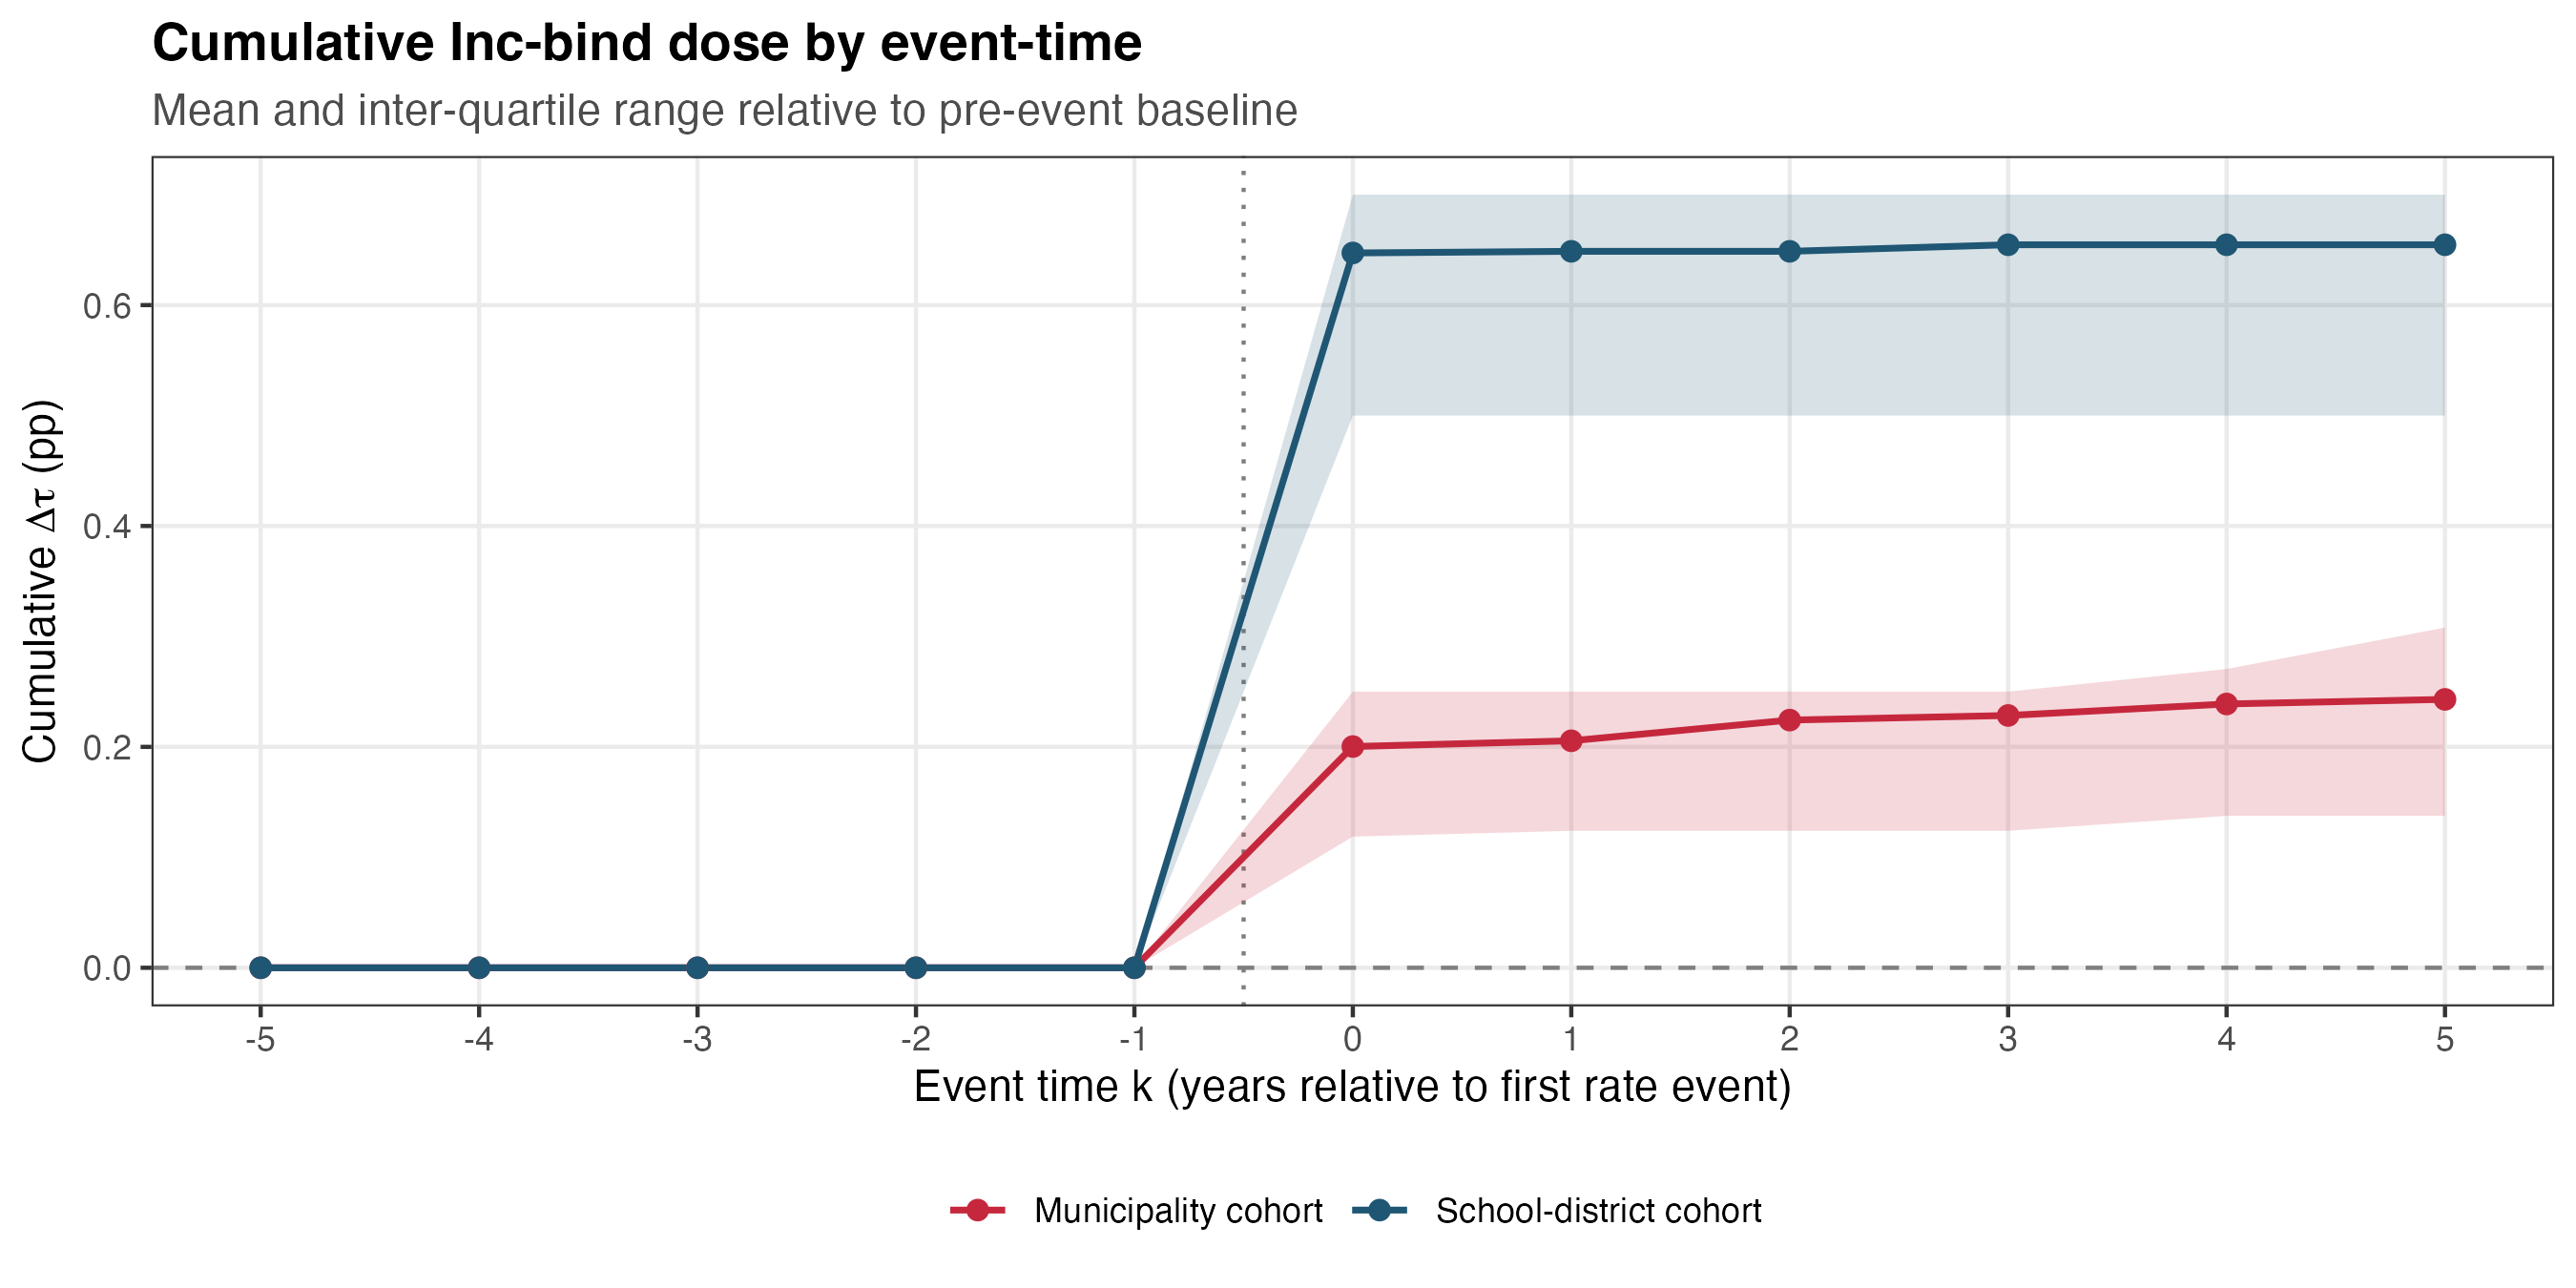
\includegraphics[width=0.85\textwidth]{../figures/support_dose_trajectory_muni_vs_sd.png}
  \begin{minipage}{0.85\textwidth}
    \footnotesize \textit{Notes:} Mean and inter-quartile range of
    cumulative dose by relative event-time $k$. The municipality
    cohort (red) reaches a mean of $0.24$ pp at $k=+5$; the
    school-district cohort (blue) reaches $0.65$ pp. Pre-event
    values are zero by construction.
  \end{minipage}
\end{figure}

Figure~\ref{fig:dose_trajectory_inc_becomes}
traces the mean cumulative resident-rate change of Inc-becomes binding on units relative to their pre-event baseline. The post-event
window shows a similar effect as figure~\ref{fig:dose_trajectory} where the school district rates sit above municipality rates at $0.60$ percentage points but the municipality rate above $0.40$ which is a much larger increase than the inc-binds grouping thus shrinking the gap between the average school district and average municipality rate. Figure~\ref{fig:dose_trajectory_inc_becomes} indicates that for an the rate to become binding the jump may primarily due to municipality rate adjustments.

\begin{figure}[H]
  \centering
  \caption{Cumulative Inc-becomes dose by event-time: municipality cohort vs.\ school-district cohort.}
  \label{fig:dose_trajectory_inc_becomes}
  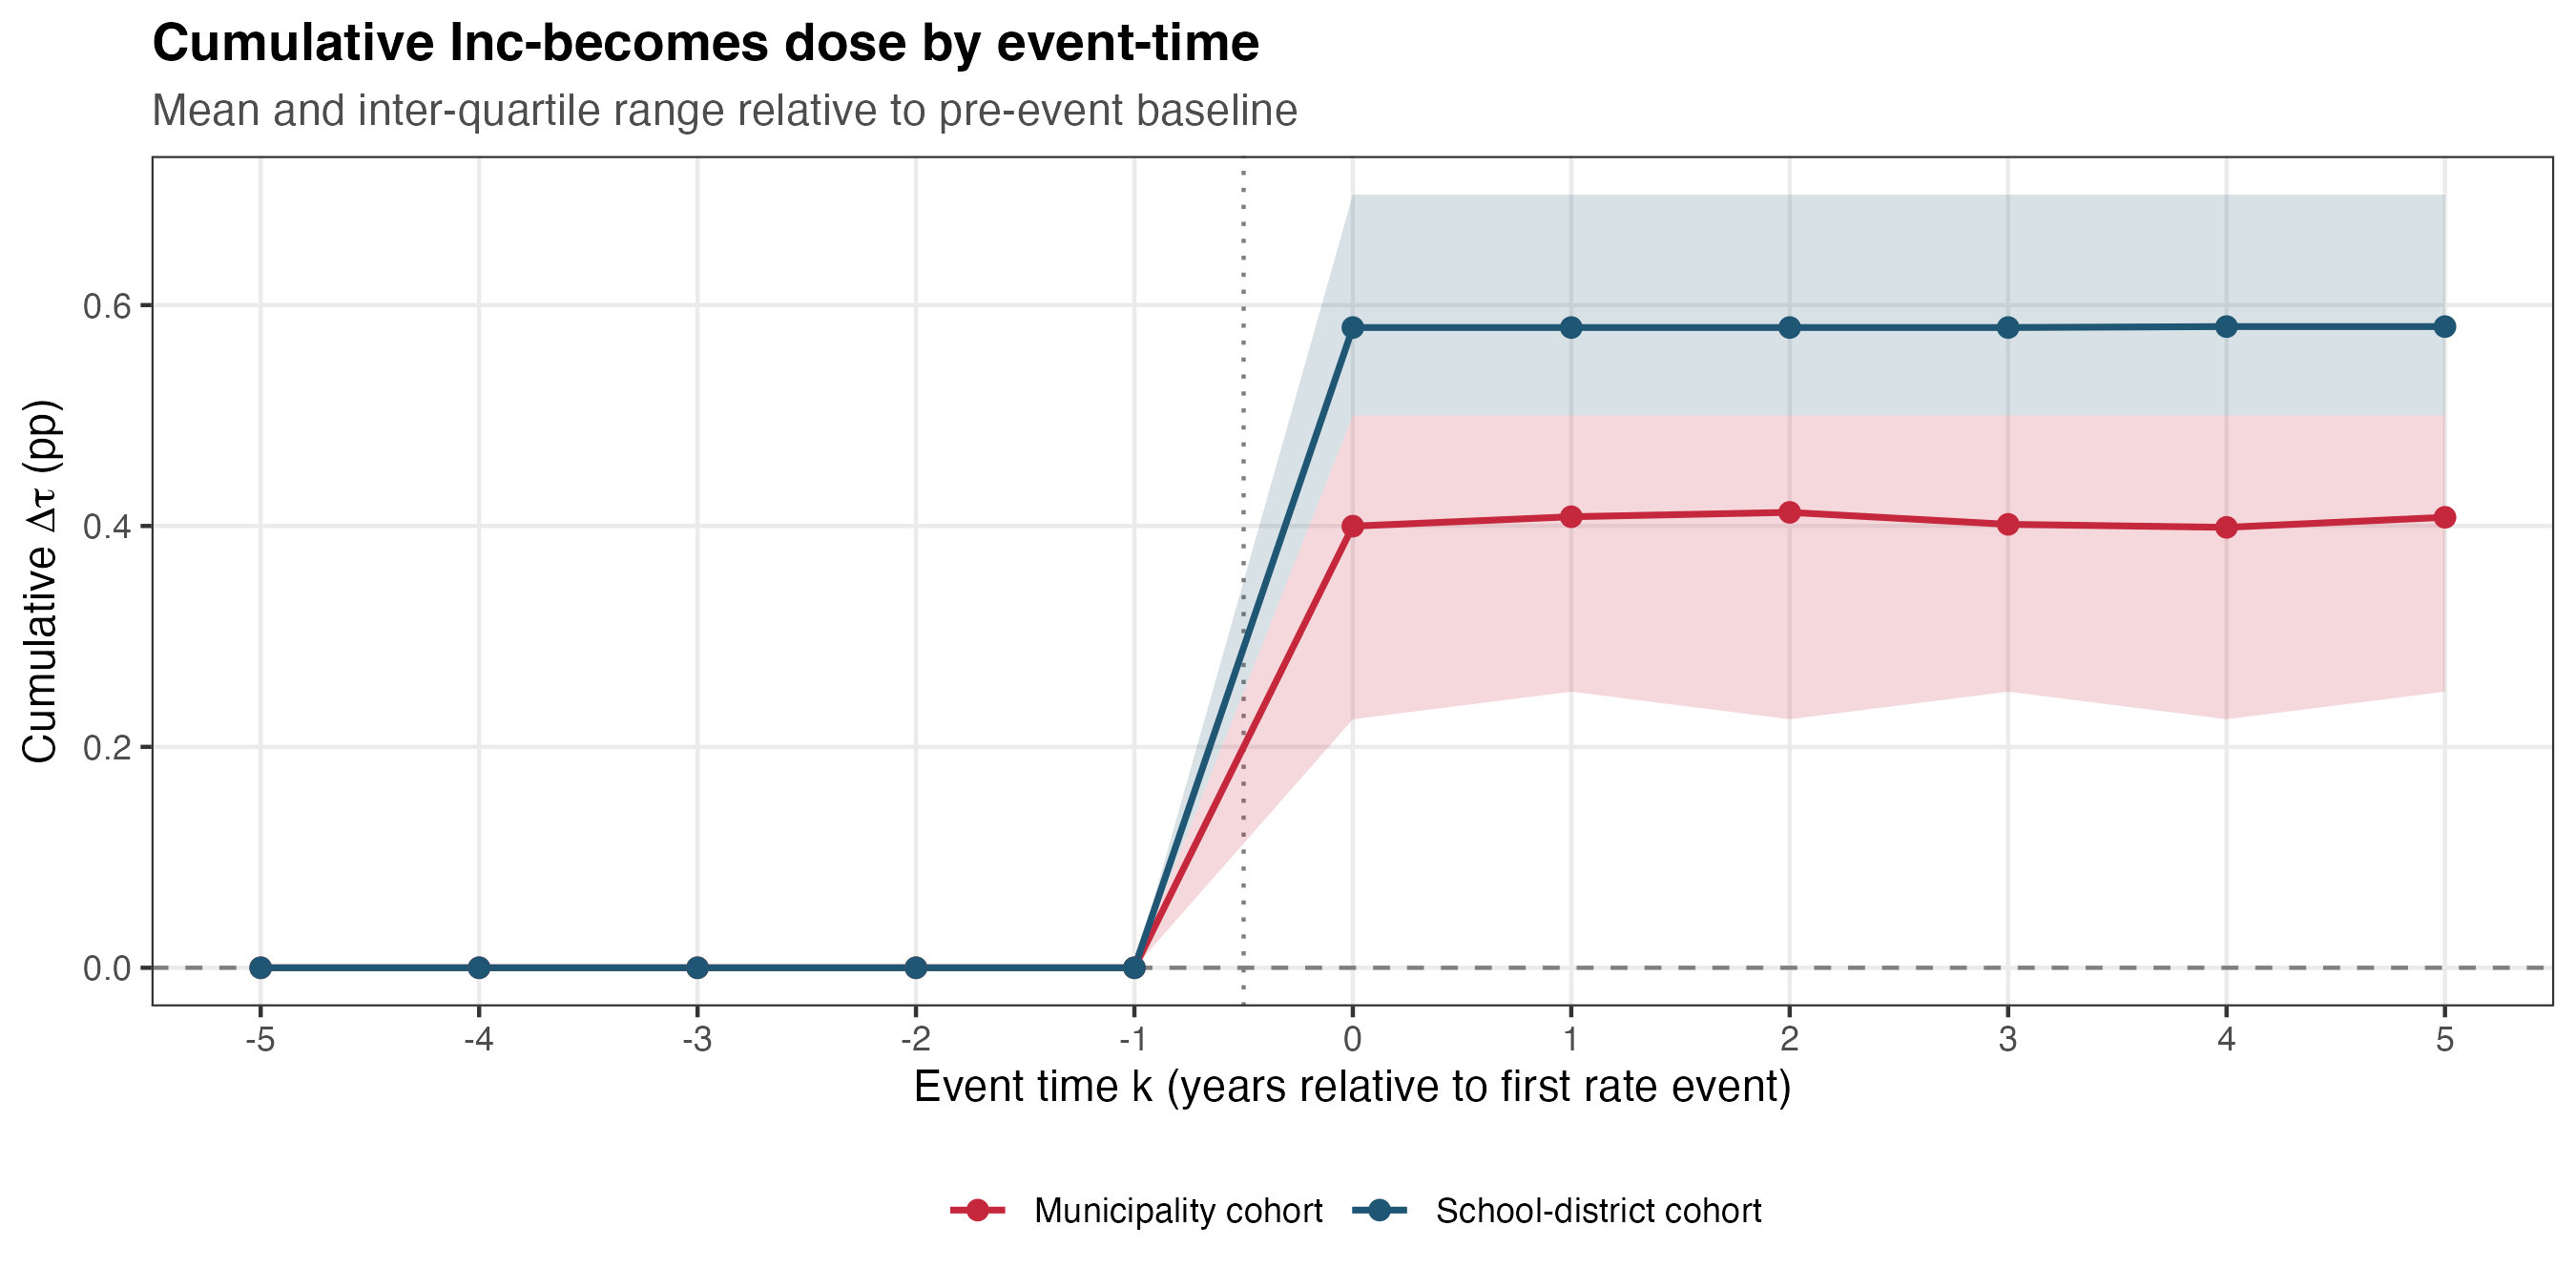
\includegraphics[width=0.85\textwidth]{../figures/support_dose_trajectory_inc_becomes.png}
  \begin{minipage}{0.85\textwidth}
    \footnotesize \textit{Notes:} As in Figure~\ref{fig:dose_trajectory}
    but for the Inc-becomes cell, where the home stack flips from
    non-binding to binding at the first event.
  \end{minipage}
\end{figure}

\subsection{Realized-Dose Event-Study Diagnostic}
\label{subsec:pretrend-diagnostics}
\label{subsec:realized-dose-es}

Equations~\ref{eq:pooled} and~\ref{eq:headline}  cannot test for pre-treatment leads
directly because $\Delta\tau^s_{it}$ is mechanically zero for all
$t < c$, so any pre-event coefficient on the dose
is also mechanically zero. I therefore run a separate
realized-dose Sun--Abraham event study on the same stacked panel
to test parallel trends, the condition recommended
for continuous-treatment DiD designs by
\citet{callaway2021} and
\citet{dechaisemartin2024} states that units with
larger eventual rate changes should not be on differentially sloped
pre-event trajectories relative to NC controls. For each cell on
rate-setter $s$ I restrict the panel to units in (NC, cell) and
run

\begin{equation}
Y_{it} = \alpha_{\tilde i} + \gamma_{\tilde t}
+ \sum_{k \neq -1} \beta^M_k\, \mathbf{1}\{\ell_{it} = k\}\,
\widetilde{D}_i
+ \mathbf{X}'_{it}\boldsymbol{\phi} + \varepsilon_{it}.
\label{eq:realized-dose-es}
\end{equation}

Two variables are new relative to Equation~\ref{eq:headline}. The
event-time index $\ell_{it} = t - c^M_i$ counts the years between
calendar year $t$ and unit $i$'s first muni-rate event year $c^M_i$,
with $\ell = -1$ (one year before the event) as the omitted
reference; in the sum below $k$ denotes a value of $\ell$, i.e.\ an
event-time, in contrast to Equation~\ref{eq:headline}, where $k$
indexed the binding cells. The realized-dose tag
$\widetilde{D}_i = \tau^M_{i, c+5} - \tau^M_{i, c-1}$ is a single number per unit where $i$'s eventual cumulative rate
change is the observed rate five years after its first event minus the
rate the year before and held fixed across all event-time years rather
than allowed to grow from zero as $\Delta\tau^M_{it}$ does in
Equation~\ref{eq:headline}. It enters the regression only through the
interaction $\mathbf{1}\{\ell_{it}=k\}\,\widetilde{D}_i$, which equals
$\widetilde{D}_i$ in the single year unit $i$ is at event-time $k$ and
zero in all its other years because that varies within unit, the
unit fixed effect (which removes only within-unit constants) does not
absorb it. Because the tag is non-zero in every event year and varies across units by eventual treatment
intensity, each pre-event $\beta^M_k$ tests whether units that
eventually take larger rate changes were already on differently sloped
trajectories. The time-varying $\Delta\tau^M_{it}$ cannot do this: it
is mechanically zero before the event, so its pre-event coefficients
are mechanically zero. The outcome $Y_{it}$, the unit-by-stack and year-by-stack
fixed effects, the control vector $\mathbf{X}_{it}$, the units of
observation, and the policy-jurisdiction clustering are the same
as in Equation~\ref{eq:headline}.

The pre-event coefficients $\beta^M_k$ for $k \leq -2$ are the
parallel-trends test: if units that eventually take large rate
changes are on differentially sloped trajectories before the rate
change, the $\beta^M_k$ at pre-event leads will be non-zero. Under
strong parallel trends they are zero. The post-event coefficients
$\beta^M_k$ for $k \geq 0$ recover the per-pp dose-response at
each event-time and average to the corresponding cell coefficient
$\beta^s_{\text{cell}}$ from Equation~\ref{eq:headline} when the
unit's rate path is a single step at the event year. I report the
joint Wald $p$-value as a single pre-trend
statistic for each cell-outcome combination.

Section~\ref{sec:results} reports the headline binding
decomposition at the municipality and the pooled-Increase
benchmark. Additional diagnostics (pre/post Act~32 split, Act~47
exclusion) are in Section~\ref{sec:robustness}.

\subsection{Property-Tax Treatment and the Concurrent-Tax Control}
\label{subsec:proptax-strategy}

The property tax enters the same municipality-level stacked design, but
as a continuous policy dose rather than a binding cell. For municipality
$i$, the treatment is the cumulative discretionary millage change since
its event, valued at the baseline CLR (Section~\ref{subsec:proptax-theory});
the event is the municipality's largest material discretionary millage
increase, which gives staggered timing across the panel. Because millage
changes nearly every year there is no never-treated pool, so the dose
enters continuously and identification is from variation in dose
\emph{magnitude}: the realized-dose event study replaces the cell$\times$dose
interaction with the eventual cumulative policy dose interacted with
event time, exactly as for the EIT, and the pre-event coefficients are
the only test of parallel trends. Where that test fails---on the
residence-count outcomes---I do not report a point estimate but instead
Rambachan--Roth honest-DiD bounds \citep{rambachanMorePlausibleApproach2023}
that treat the observed pre-trend as a bias budget; where it passes---on
the local-employment composition share and the workplace counts---I
report the dose-response coefficient.

Each leg controls for the concurrent change in the other tax. The EIT
binding-decomposition regression includes the concurrent cumulative
property dose, and the property-tax regression includes the concurrent
cumulative EIT dose, each as a continuous control over the same event
window. This is a nuisance control, not a joint identification of both
elasticities in one model: the two taxes are estimated in separate
designs and compared, because the property tax's residence-count margin
is not cleanly identified and could not carry a co-equal coefficient.
The municipal and school-district resident EIT changes are weakly
correlated ($-0.12$) and the discretionary-millage and EIT-rate changes
co-occur only modestly, so the concurrent controls move the estimates
little; I report the comparison both with and without them.

%==========================================================
\section{Results}
\label{sec:results}
%==========================================================

I report results in two layers. First,
Section~\ref{subsec:results-pooled} presents the pooled Inc
benchmark, which approximates what a conventional local-tax design
would recover by averaging across all rate-increase events without
distinguishing whether they bind. Second,
Section~\ref{subsec:results-decomp} reports the binding
decomposition at the municipality level. The central empirical
comparison is between the Inc-bind cell (where the statutory rate
change moves the worker's bill) and the Inc-nobind cell (where it
does not), with Inc-nobind serving as the within-design placebo.
Dec cells are not estimated: the cohort is thin
(5 Dec-bind, 3 Dec-becomes-non, 11 Dec-nobind) and the
realized-dose pre-trend rejects parallel trends on every Dec
outcome (Wald $p<0.001$), so the Dec coefficients cannot be
interpreted as causal. The pre-/post-Act-32 enforcement-break split
appears in the Robustness section.

\subsection{Pooled-Increase Benchmark}
\label{subsec:results-pooled}

I first report the pooled-Increase specification from
Equation~(\ref{eq:pooled}), which collapses each rate-setter to a
single direction tag for rate increases. The pooled coefficients
are useful because they approximate the estimand in a conventional
local-tax design where the average per-pp dose-response of a
municipality-rate change and an SD-rate change without
distinguishing whether the rate change moves the worker's bill.

Table~\ref{tab:pooled_per_pp_cousub} reports the per-pp pooled
coefficients at the municipality level. The table reports the two
coefficients of interest per outcome: the municipality resident-rate
Inc effect $\beta^M_{\text{Inc}}$ and the school-district-rate Inc
analogue $\beta^{SD}_{\text{Inc}}$.

\begin{table}[H]
  \centering
  \caption{Pooled Inc/Dec headline --- municipality level (per pp)}
  \label{tab:pooled_per_pp_cousub}
  \small
  \resizebox{\textwidth}{!}{
  \begin{tabular}{lcccc}
    \toprule
    Outcome & Log(work in own muni) & Log(in-commuters) & Log(employed residents) & Share live in muni \\
    \midrule
    \textbf{Municipality rate ($\tau^{M}$)} & & & & \\
    \quad $\Delta\tau > 0$ (Inc) & -0.228\sym{***} & -0.209\sym{***} & -0.035 & -0.019\sym{**} \\
                           & (0.058) & (0.056) & (0.033) & (0.008) \\
    \quad $\Delta\tau < 0$ (Dec) & 0.260\sym{**} & 0.014 & 0.058 & 0.022 \\
                           & (0.107) & (0.143) & (0.138) & (0.019) \\
    \textbf{School district rate ($\tau^{SD}$)} & & & & \\
    \quad $\Delta\tau > 0$ (Inc) & 0.128\sym{*} & 0.105 & 0.051 & 0.007 \\
                           & (0.070) & (0.067) & (0.038) & (0.005) \\
    \quad $\Delta\tau < 0$ (Dec) & -0.310\sym{***} & -0.170\sym{**} & 0.020 & -0.003 \\
                           & (0.110) & (0.076) & (0.051) & (0.007) \\
    \midrule
    $N$ & 218,677 & 239,023 & 242,722 & 239,033 \\
    $R^2$ & 0.964 & 0.959 & 0.981 & 0.823 \\
    Within $R^2$ & 0.001 & 0.001 & 0.001 & 0.001 \\
    Dep.\ mean & 3.677 & 5.847 & 6.697 & 0.093 \\
    Dep.\ SD & 1.934 & 1.887 & 1.299 & 0.076 \\
    \bottomrule
  \end{tabular}
  }
  \vspace{0.3em}
  \begin{minipage}{0.95\textwidth}
    \footnotesize \textit{Notes:} Cluster-robust standard errors in parentheses. Each regression includes both rate-setters' direction-pooled treatments jointly; the four reported coefficients are $\beta^M_{\text{Inc}}$, $\beta^M_{\text{Dec}}$, $\beta^{SD}_{\text{Inc}}$, $\beta^{SD}_{\text{Dec}}$. $^{*}p<0.10$, $^{**}p<0.05$, $^{***}p<0.01$.
  \end{minipage}
\end{table}


The muni-rate Inc coefficient on log live-and-work is
$-0.287^{***}$, and the count outcomes move together. Log
in-commuters is $-0.256^{***}$ and log total jobs $-0.283^{***}$,
and the share of workers who both live and work in their own
municipality is a small $-0.020^{*}$. The cell decomposition in
Section~\ref{subsec:results-decomp} shows this aggregate is driven
by Inc-bind ($-0.573^{***}$ on log live-and-work) with Inc-becomes
and Inc-nobind averaged in. The pooled-Inc ES on log live-and-work
fails parallel trends (Wald $p=0.002$, Table~\ref{tab:es_pooled_cousub}),
because the Inc-becomes and Inc-nobind munis enter with non-zero
pre-event trajectories. The Inc-bind cell on its own passes
pre-trends cleanly ($p=0.33$, Section~\ref{subsubsec:decomp-es}),
which is why the decomposition rather than the pooled coefficient
carries the causal claim. The SD-rate Inc coefficients are positive
and weak ($+0.128^{*}$ on log live-and-work), sign-reversed relative
to the muni-rate finding. Aggregating across a school district mixes
the rate-changing municipality (where residents may move out) with
non-changing munis in the same SD (which may gain residents from
within-SD movers).

\subsubsection{Realized-dose ES benchmark diagnostic}
\label{subsubsec:pooled-es}

Table~\ref{tab:es_pooled_cousub} reports the ATT summary of the
muni-level pooled realized-dose event study, with the
cluster-robust Wald pre-trend $p$-value for the joint null
$\beta_k = 0$ at $k \leq -2$.
Figure~\ref{fig:pooled_es_muni_only} plots the event-time path.

\begin{table}[!htbp]
  \centering
  \caption{Pooled realized-dose event study --- municipality level.}
  \label{tab:es_pooled_cousub}
  \footnotesize
  \renewcommand{\arraystretch}{0.85}
  \resizebox{\textwidth}{!}{
  \begin{tabular}{lcccc}
    \toprule
    Direction & Log(work in own muni) & Log(in-commuters) & Log(employed residents) & Share live in muni \\
    \midrule
    \textbf{Inc} (post) & -0.232 & -0.254 & -0.029 & -0.014 \\
                      & (0.039) & (0.039) & (0.020) & (0.005) \\
    \textbf{Inc} (pre) & 0.068 & 0.069 & -0.004 & 0.002 \\
                      & (0.032) & (0.055) & (0.038) & (0.007) \\
    \textbf{Inc} Wald $p$ & 0.0012 & 0.0454 & 0.0482 & 0.5333 \\
    \textbf{Dec} (post) & 0.686 & 0.393 & 0.111 & 0.002 \\
                      & (0.207) & (0.126) & (0.045) & (0.006) \\
    \textbf{Dec} (pre) & 0.189 & -0.152 & 0.182 & -0.002 \\
                      & (0.234) & (0.113) & (0.043) & (0.005) \\
    \textbf{Dec} Wald $p$ & $<\!0.0001$ & $<\!0.0001$ & $<\!0.0001$ & $<\!0.0001$ \\
    \midrule
    \multicolumn{5}{l}{\textit{Diagnostics}} \\
    $N$              & 179,169 & 195,702 & 198,654 & 195,711 \\
    $R^2$            & 0.9643 & 0.9605 & 0.9811 & 0.8281 \\
    Within $R^2$     & 0.0013 & 0.0025 & 0.0012 & 0.0016 \\
    Dep.\ mean       & 3.6670 & 5.8570 & 6.6980 & 0.0920 \\
    Dep.\ SD         & 1.9320 & 1.8810 & 1.2960 & 0.0740 \\
    \bottomrule
  \end{tabular}
  }
  \vspace{0.3em}
  \begin{minipage}{0.95\textwidth}
    \footnotesize \textit{Notes:} Cluster-robust standard errors in parentheses. Post = mean of $\beta_k$ for $k = 0, \ldots, 5$; pre = mean for $k \leq -2$. Wald $p$ is the cluster-robust joint test of $H_0\colon \beta_k = 0$ across pre-event $k$. $^{*}p<0.10$, $^{**}p<0.05$, $^{***}p<0.01$.
  \end{minipage}
\end{table}


The pooled-Inc post-event coefficient on log live-and-work is
$-0.257$, with a small but non-zero pre-event lead, and the joint
Wald $p=0.002$ rejects strong parallel trends. As above, the rejection
reflects Inc-becomes and Inc-nobind selection rather than a problem
with Inc-bind on its own, which the decomposition isolates.

The other three pooled outcomes in Table~\ref{tab:es_pooled_cousub}
and Figure~\ref{fig:pooled_es_muni_only} move with the live-and-work
result. The pooled-Inc post on log in-commuters is $-0.247$
($p=0.016$) and on log total jobs $-0.271$ ($p=0.039$). The three
count measures contract together by roughly a quarter of a log point
per pp ($0.247$--$0.271$), which points to a single workplace-side
margin rather than an outcome-specific artifact. The share of workers
who both live and work in the municipality is small and negative
($-0.019$, $p=0.14$) and is the only pooled outcome whose joint
pre-trend test does not reject. Muni-level share outcomes mix
denominator dynamics with binding-channel sorting, and enter as
supporting evidence rather than as primary identification.

These pooled magnitudes average over municipalities whose rate
changes do and do not move the worker's bill, and three of the four
reject the joint pre-trend test. The realized-dose decomposition in
Section~\ref{subsec:results-decomp} addresses both problems at once.
It isolates the Inc-bind cell, where the rate increase actually
pushes the home stack above the work rate, from the Inc-becomes and
Inc-nobind municipalities that contribute the non-zero leads. There
the live-and-work effect sharpens to $-0.573^{***}$ on a cell with
clean realized-dose pre-trends (joint Wald $p=0.33$), while the
within-design placebo (Inc-nobind) is null. A large
pre-trend-clean effect in the binding cell beside a null placebo is
why the decomposition rather than the pooled coefficient carries the
causal claim.

\begin{figure}[H]
  \centering
  \caption{Municipality-level pooled realized-dose event study.}
  \label{fig:pooled_es_muni_only}
  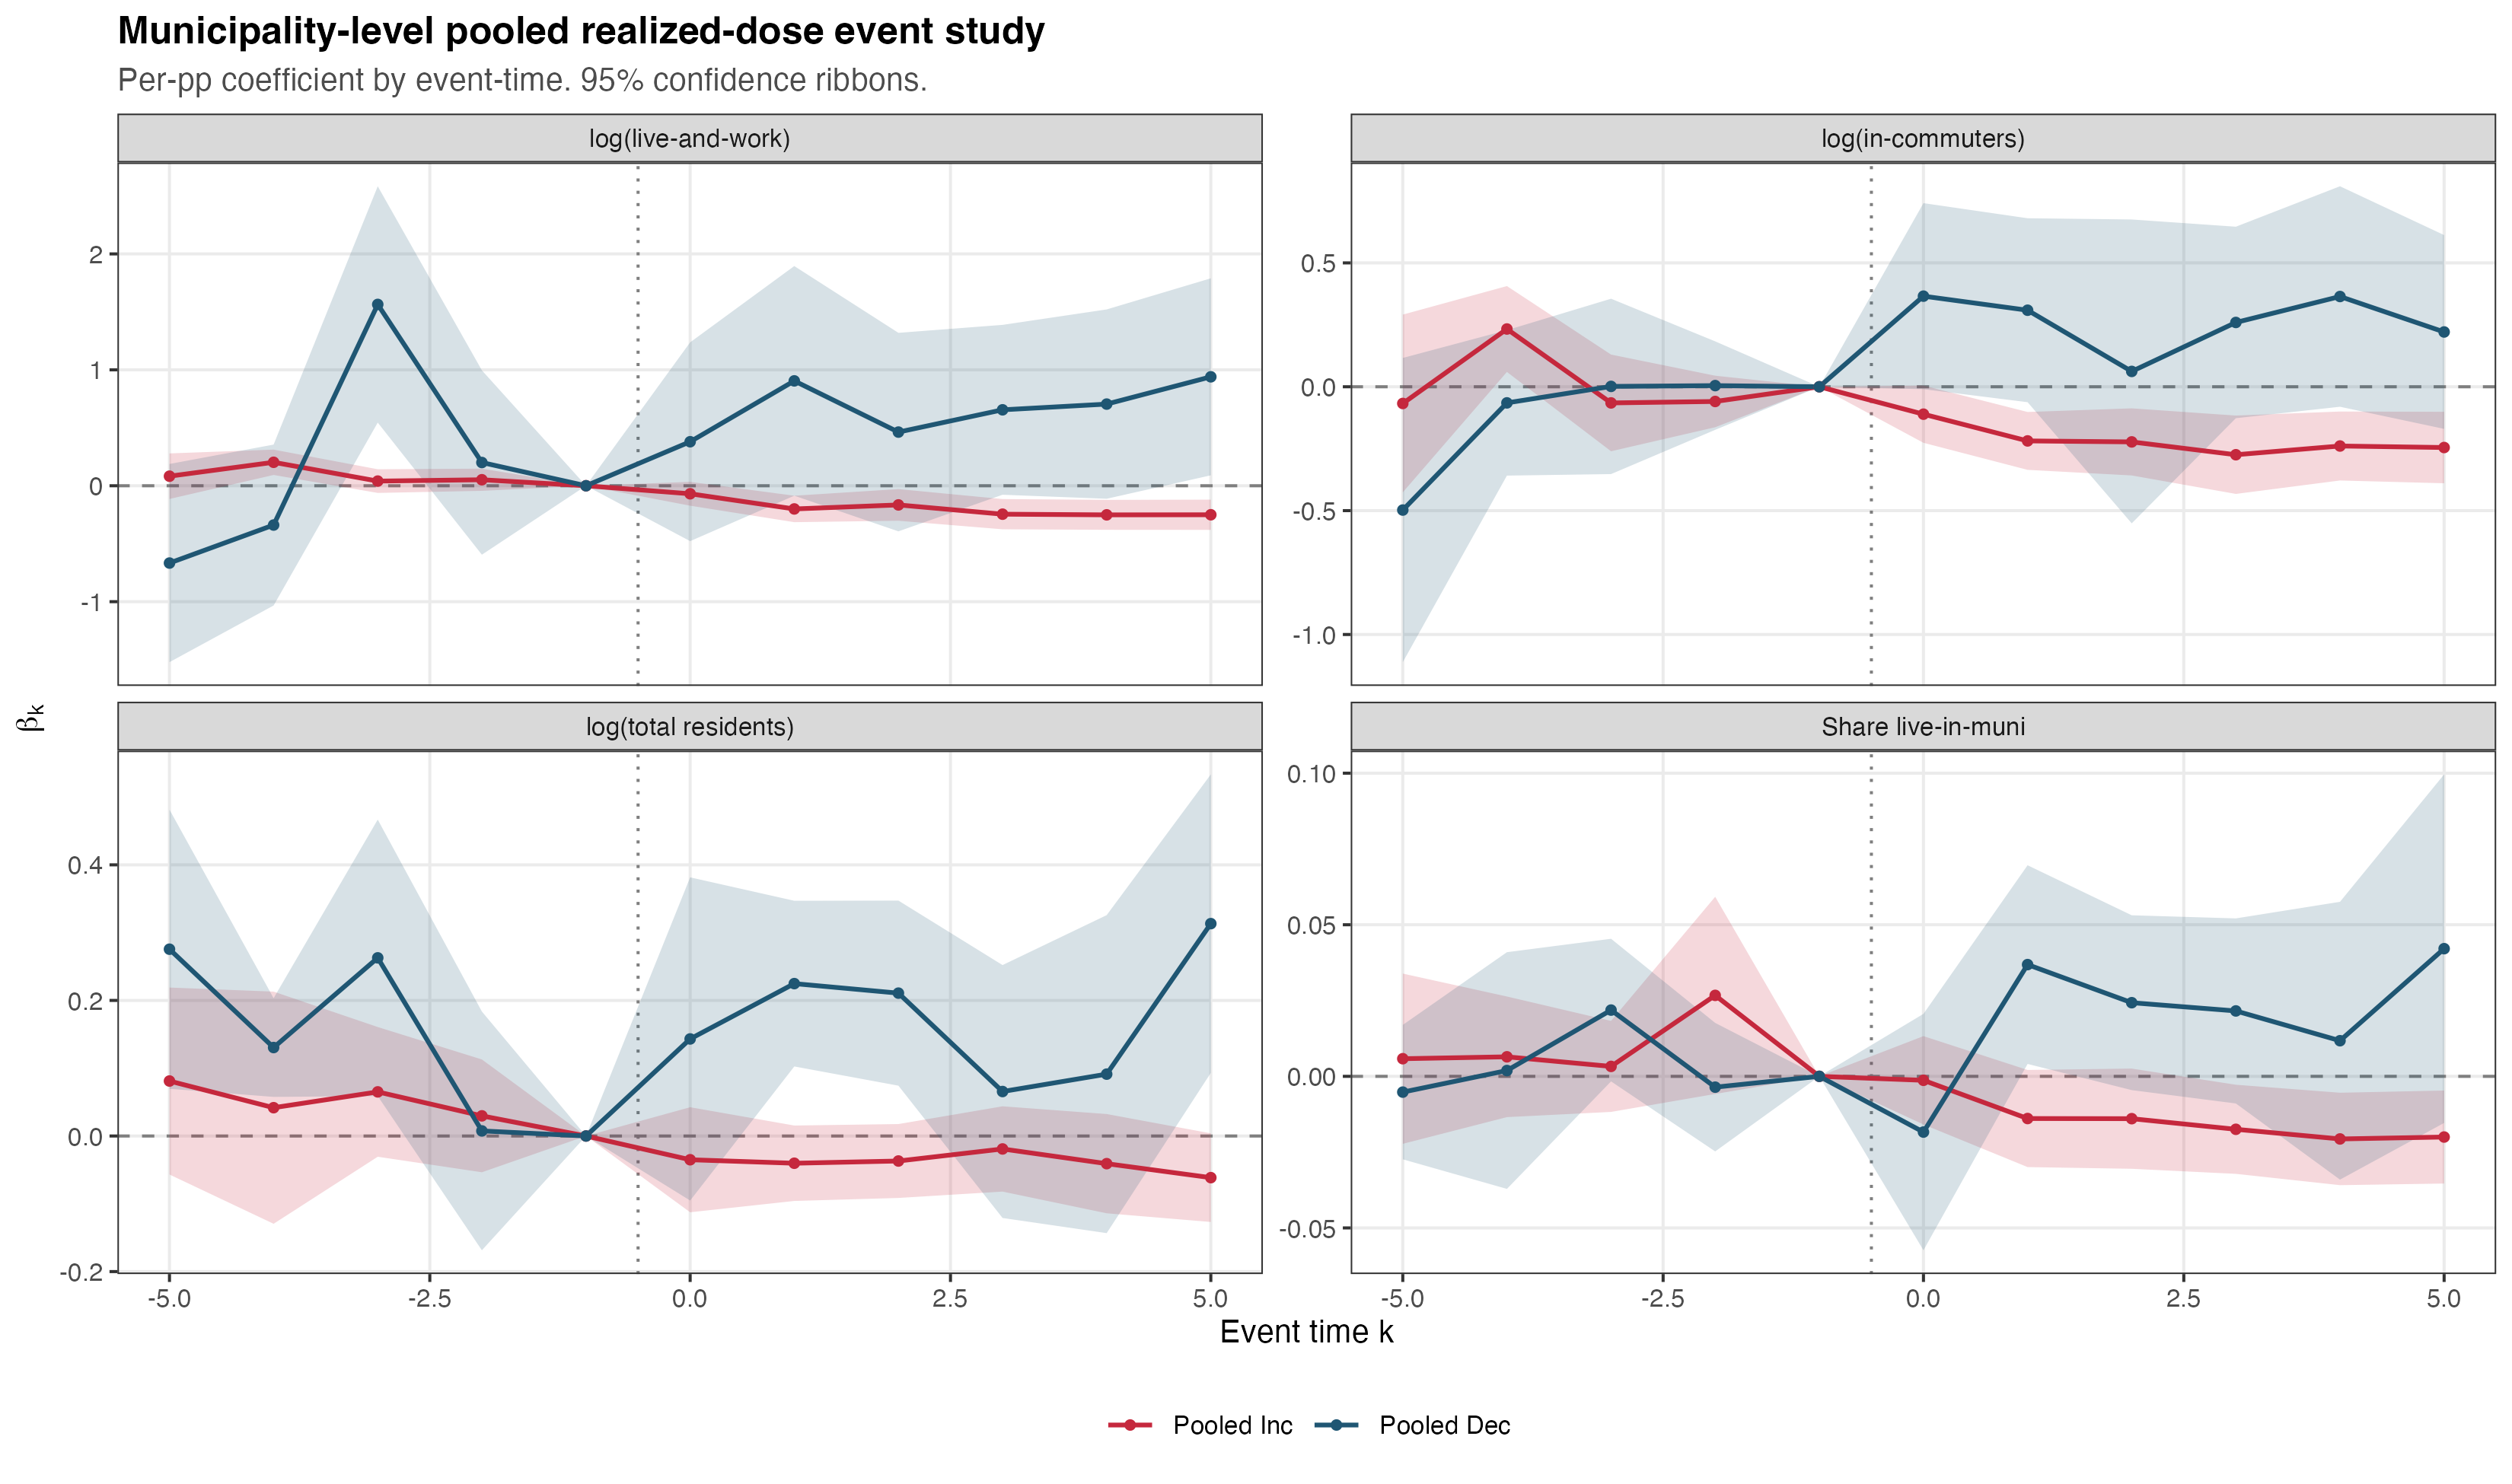
\includegraphics[width=0.95\textwidth]{../figures/pooled_es_muni_only.png}
  \begin{minipage}{0.95\textwidth}
    \footnotesize \textit{Notes:} Per-pp realized-dose coefficient at each event-time for the pooled Inc cohort. Ribbon is the 95\% CI; $k=-1$ omitted as the reference period.
  \end{minipage}
\end{figure}

\subsection{Binding Decomposition}
\label{subsec:results-decomp}
\label{subsec:results-headline}

The decomposition is estimated at the municipality level. Both
rate-setter treatments enter the same joint regression: each
muni-year is assigned its own resident rate $\tau^M$ at local
level and $\max(\tau^{SD})$ across the school districts the muni
reports to. Table~\ref{tab:headline_muni_combined}
reports both sets of cell coefficients from the same joint
regression in a single panel: the muni resident-rate cells (top
panel) are the headline causal claim, and the SD resident-rate
cells (bottom panel) are reported alongside as co-treatment from
the identical specification.

\begin{table}[!htbp]
  \centering
  \caption{Municipality-level dose-response: muni and SD resident-rate cells (joint regression)}
  \label{tab:headline_muni_combined}
  \footnotesize
  \renewcommand{\arraystretch}{0.9}
  \resizebox{\textwidth}{!}{
  \begin{tabular}{lcccc}
    \toprule
    Cell & Log(work in own muni) & Log(in-commuters) & Log(employed residents) & Share live in muni \\
    \midrule
    \multicolumn{5}{l}{\textit{Muni resident rate ($\tau^M$)}} \\
    \textbf{Inc-bind} & -0.573\sym{***} & -0.412\sym{***} & -0.104\sym{**} & -0.058\sym{***} \\
                      & (0.162) & (0.126) & (0.043) & (0.020) \\
    \textbf{Inc-becomes} & -0.250\sym{***} & -0.247\sym{***} & -0.042 & -0.014 \\
                      & (0.056) & (0.055) & (0.027) & (0.011) \\
    \textbf{Inc-nobind} & -0.073 & 0.233 & 0.382\sym{**} & -0.037 \\
                      & (0.143) & (0.302) & (0.188) & (0.032) \\
    \midrule
    \multicolumn{5}{l}{\textit{School district rate ($\tau^{SD}$)}} \\
    \textbf{Inc-bind} & 0.165 & 0.159 & 0.057 & 0.005 \\
                      & (0.109) & (0.096) & (0.049) & (0.007) \\
    \textbf{Inc-becomes} & 0.084 & 0.086 & 0.031 & 0.007 \\
                      & (0.095) & (0.089) & (0.056) & (0.007) \\
    \midrule
    \multicolumn{5}{l}{\textit{Diagnostics}} \\
    $N$           & 174,929 & 191,405 & 194,533 & 191,413 \\
    $R^2$         & 0.963 & 0.959 & 0.980 & 0.825 \\
    Within $R^2$  & 0.001 & 0.001 & 0.001 & 0.001 \\
    Dep.\ mean    & 3.659 & 5.836 & 6.686 & 0.092 \\
    Dep.\ SD      & 1.926 & 1.883 & 1.296 & 0.075 \\
    \bottomrule
  \end{tabular}
  }
  \vspace{0.3em}
  \begin{minipage}{0.95\textwidth}
    \footnotesize \textit{Notes:} Stacked-DiD; muni$\times$stack and year$\times$stack FE; SE clustered at muni. Both rate-setters enter the same joint regression; the table reports both sets of cell$\times$dose coefficients. Cells omitted (no estimable coefficients): Inc-nobind. $^{*}p<0.10$, $^{**}p<0.05$, $^{***}p<0.01$.
  \end{minipage}
\end{table}


The Inc-bind cell has clean realized-dose pre-trends on the three
count outcomes (table~\ref{tab:es_realized_cousub}). To understand the results, I translate them using the mean cumulative resident-rate increase at
$k=+5$ for the 24 Inc-bind municipalities which is $0.24$ pp
(Figure~\ref{fig:dose_trajectory}). At that typical dose, the
Inc-bind coefficient on log live-and-work implies a
$0.24\times(-0.573)=-0.14$ log-point change, or $13\%$ reduction in
residents who both live and work in their own municipality. The
dependent-variable mean of $3.66$ corresponds to about $39$ workers ($e^{3.66}$) in the typical muni, so a $13\%$ drop is
roughly $5$ fewer live-and-work workers per Inc-bind muni over
five years. The same scaling on log in-commuters
($\beta=-0.412$) implies $10\%$ reduction in-commuters, or about 34 fewer
in-commuters relative to a typical baseline of
$343$. The same scaling on log total jobs ($\beta=-0.490$) implies
about $-11\%$ in jobs located in the municipality; the fact that the estimate for the
live-and-work count falls by more than the workplace as a whole
($-13\%$ vs $-11\%$) is residential displacement net of the general
labor-market contraction.

The share of workers who both live and work in their own
municipality is the most direct read on the binding-rule mechanism,
and it moves in the predicted direction. The Inc-bind coefficient is
$-0.058^{***}$ (Wald $p=0.003$), so residents' share of local
employment falls even net of the labor-market contraction. At the
typical Inc-bind event the $0.24$ pp cumulative increase implies a
$0.24\times(-0.058)$ approximately a $-0.014$ change in the share, a drop of
about $1.4$ percentage points from a baseline mean of $9.2\%$ which is about a
$15\%$ relative decline. Against the $380$ ($e^{5.94}$) jobs
located in a typical municipality that is roughly $5$ fewer of those
jobs held by residents, and is also the same residential displacement the count
outcomes show, now measured net of the overall decline in jobs. I read this effect as causal even though it fails the pre-trends test. This is due to swings in the pre-period that for the most part not statistically significant. 

The Inc-becomes cell produces significant coefficients on the
same two log count outcomes ($-0.250^{***}$ on log live-and-work;
$-0.247^{***}$ on log in-commuters) but the realized-dose
pre-trend on both fails the parallel-trends test (Wald $p=0.0001$
and $p<0.0001$), though the joint rejection is driven almost
entirely by a single anomalous pre-event lead ($k=-4$) rather than
a sustained differential trend. I therefore read
Inc-becomes as suggestive rather than purely causal.

The Inc-nobind cell is the within-design placebo and has 14 municipalities
whose home stack stays below the work rate after
the rate hike, so the mechanism predicts that there should not be any movers given the worker's
bill never moves. The placebo passes on all three count outcomes: Inc-nobind on log live-and-work is $-0.073$,
on log in-commuters $+0.233$, and on log total jobs
$+0.193$, all statistically indistinguishable from
zero, so the within-design placebo holds across the count outcomes.

The SD-rate cells in the same regression produce postive effects that are not statistically signficant. The results
are thus sign-reversed relative to the muni-rate finding and loses power relative to the aggregate results in table~\ref{tab:es_pooled_cousub}. The estimates suggest that in general tax increases from school districts produce positive sorting into the city but cannot decompose that effect for whether it is binding or not. This may partly be due to the SD-rate entering the regression as a co-treatment
but does not by itself identify the residential sorting response.

\subsubsection{Realized-dose ES decomposition diagnostics}
\label{subsubsec:decomp-es}

The realized-dose event study disaggregates the pooled pre-trend
by cell. Table~\ref{tab:es_realized_cousub} reports each cell's
post-event ATT, pre-event lead, and the joint pre-trend Wald $p$
across the four muni outcomes, and the pre-trend numbers quoted in
Section~\ref{subsec:results-decomp} are drawn from it. Inc-bind on
log live-and-work passes the strong parallel-trends standard.
Pre-event coefficients are individually not statistically significant. The post-event path is
uniformly negative and deepens through $k=4$. Inc-becomes and Inc-nobind
fail pre-trends ($p<0.001$ on both). This is what the
mechanism predicts. Cohorts selected into rate changes
that flip the binding state or stay non-binding are munis on
differentially sloped pre-event trajectories. Inc-bind is the
only cell that survives the strong parallel-trends standard.

\begin{table}[!htbp]
  \centering
  \caption{Realized-dose event study by binding-state cell --- municipality level.}
  \label{tab:es_realized_cousub}
  \footnotesize
  \renewcommand{\arraystretch}{0.85}
  \resizebox{\textwidth}{!}{
  \begin{tabular}{lcccc}
    \toprule
    Cell & Log(work in own muni) & Log(in-commuters) & Log(total jobs) & Share live in muni \\
    \midrule
    \textbf{Inc-bind} (post) & -0.762 & -0.498 & -0.591 & -0.069 \\
                      & (0.095) & (0.080) & (0.076) & (0.015) \\
    \textbf{Inc-bind} (pre) & -0.072 & 0.119 & 0.093 & -0.020 \\
                      & (0.068) & (0.088) & (0.080) & (0.012) \\
    \textbf{Inc-bind} Wald $p$ & 0.3318 & 0.6970 & 0.7925 & 0.0034 \\
    \textbf{Inc-becomes} (post) & -0.171 & -0.194 & -0.208 & -0.012 \\
                      & (0.037) & (0.039) & (0.038) & (0.004) \\
    \textbf{Inc-becomes} (pre) & 0.075 & 0.081 & 0.082 & -0.002 \\
                      & (0.028) & (0.057) & (0.054) & (0.008) \\
    \textbf{Inc-becomes} Wald $p$ & 0.0001 & $<\!0.0001$ & $<\!0.0001$ & 0.1877 \\
    \textbf{Inc-nobind} (post) & 0.044 & -0.057 & -0.068 & -0.012 \\
                      & (0.080) & (0.077) & (0.073) & (0.007) \\
    \textbf{Inc-nobind} (pre) & 0.053 & -0.782 & -0.706 & 0.069 \\
                      & (0.151) & (0.244) & (0.216) & (0.027) \\
    \textbf{Inc-nobind} Wald $p$ & $<\!0.0001$ & $<\!0.0001$ & $<\!0.0001$ & $<\!0.0001$ \\
    \midrule
    \multicolumn{5}{l}{\textit{Diagnostics}} \\
    $N$              & 163,014 & 178,042 & 178,050 & 178,050 \\
    \bottomrule
  \end{tabular}
  }
  \vspace{0.3em}
  \begin{minipage}{0.95\textwidth}
    \footnotesize \textit{Notes:} Cluster-robust standard errors in parentheses. Post = mean of $\beta_k$ for $k = 0, \ldots, 5$; pre = mean for $k \leq -2$. Wald $p$ is the cluster-robust joint test of $H_0\colon \beta_k = 0$ across pre-event $k$. Per-cell decomposition of the muni-level realized-dose ES; each cell is run as a separate regression on \{NC, cell\}. Inc-bind is the load-bearing cell, with clean pre-trends on the three count outcomes. $^{*}p<0.10$, $^{**}p<0.05$, $^{***}p<0.01$.
  \end{minipage}
\end{table}


\begin{figure}[H]
  \centering
  \caption{Municipality-level realized-dose event study on log live-and-work, by cell.}
  \label{fig:es_realized_muni_live_work}
  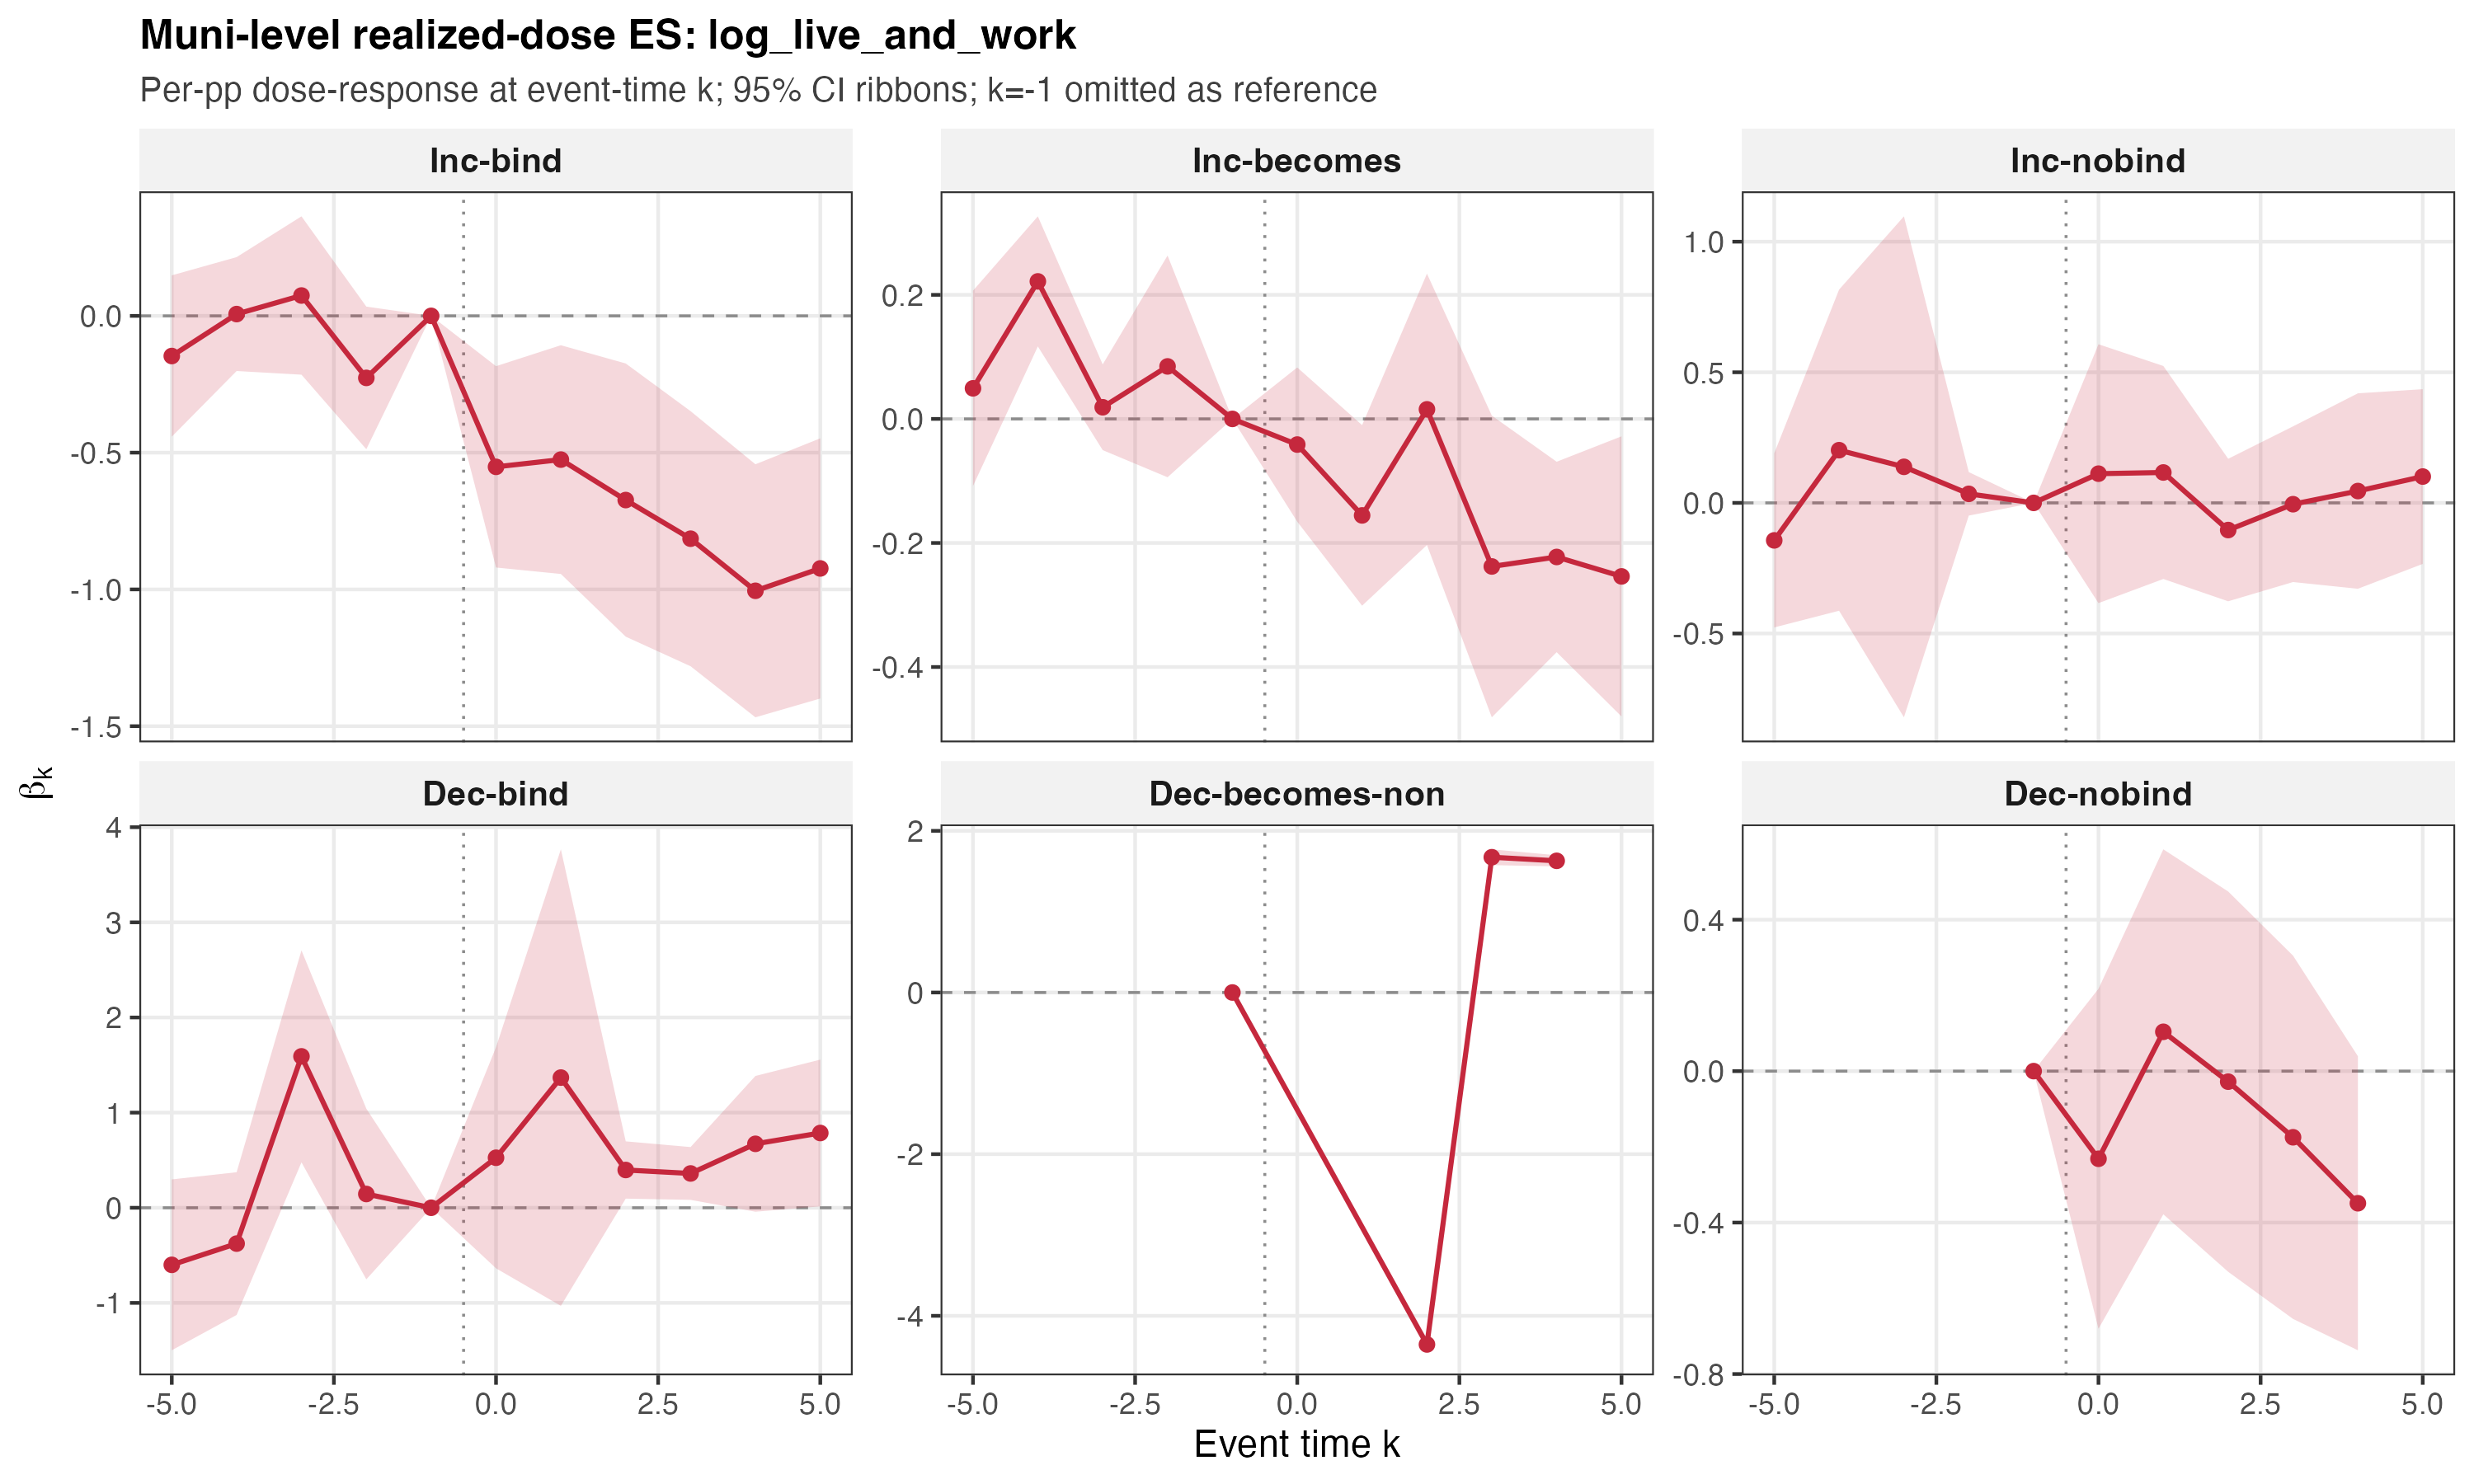
\includegraphics[width=0.95\textwidth]{../figures/es_realized_log_live_and_work.png}
  \begin{minipage}{0.95\textwidth}
    \footnotesize \textit{Notes:} Per-pp coefficient at each event-time, faceted by cell. Inc-bind pre-event Wald $p=0.33$; post path uniformly negative, deepening through $k=4$.
  \end{minipage}
\end{figure}

%==========================================================
\subsection{Property Tax: No Detectable Sorting on the Clean Margins}
\label{subsec:results-proptax}

The property tax is estimated on the same municipalities with the
policy-driven effective-rate dose (median effective rate about $2.1\%$
of market value). Its realized-dose pre-trend splits cleanly by outcome
(Figure~\ref{fig:proptax_es}). The local-employment composition share
and the workplace counts show no differential pre-trend across dose
magnitudes (joint Wald $p=0.35$, $0.97$, $0.97$), but the residence
counts do: municipalities that go on to raise the property tax are
already on diverging resident-population paths beforehand (log
live-and-work Wald $p=0.05$, log employed residents $p=0.01$). The same
diagnostic run on the EIT shows no such residence-scale divergence, so
the contamination is a whole-municipality residential trajectory, not a
composition shift, and a finer geography would not absorb it because the
treatment is municipality-wide. I therefore report the residence-count
margins as honest-DiD bounds and the composition and workplace margins
as point estimates.

On the cleanly identified margins the property tax shows \emph{no
detectable} sorting response: the dose-response coefficient is
statistically indistinguishable from zero on the composition share
($-0.001$, $p=0.26$), on log total jobs ($-0.021$, $p=0.42$), and on log
in-commuters ($-0.020$, $p=0.44$). On the contaminated residence-count
margins, the Rambachan--Roth bounds (relative-magnitude $\bar M=1$)
include zero while ruling out an EIT-sized effect---per \$1{,}000 of
annual tax, $[-0.275, +0.201]$ for log live-and-work and $[-0.131,
+0.123]$ for log residents. So the residence margin is unidentified, not
a clean null: it bounds the response well below the EIT but cannot
distinguish a small effect from none.

\begin{figure}[H]
  \centering
  \caption{Property-tax realized-dose event study, by outcome type}
  \label{fig:proptax_es}
  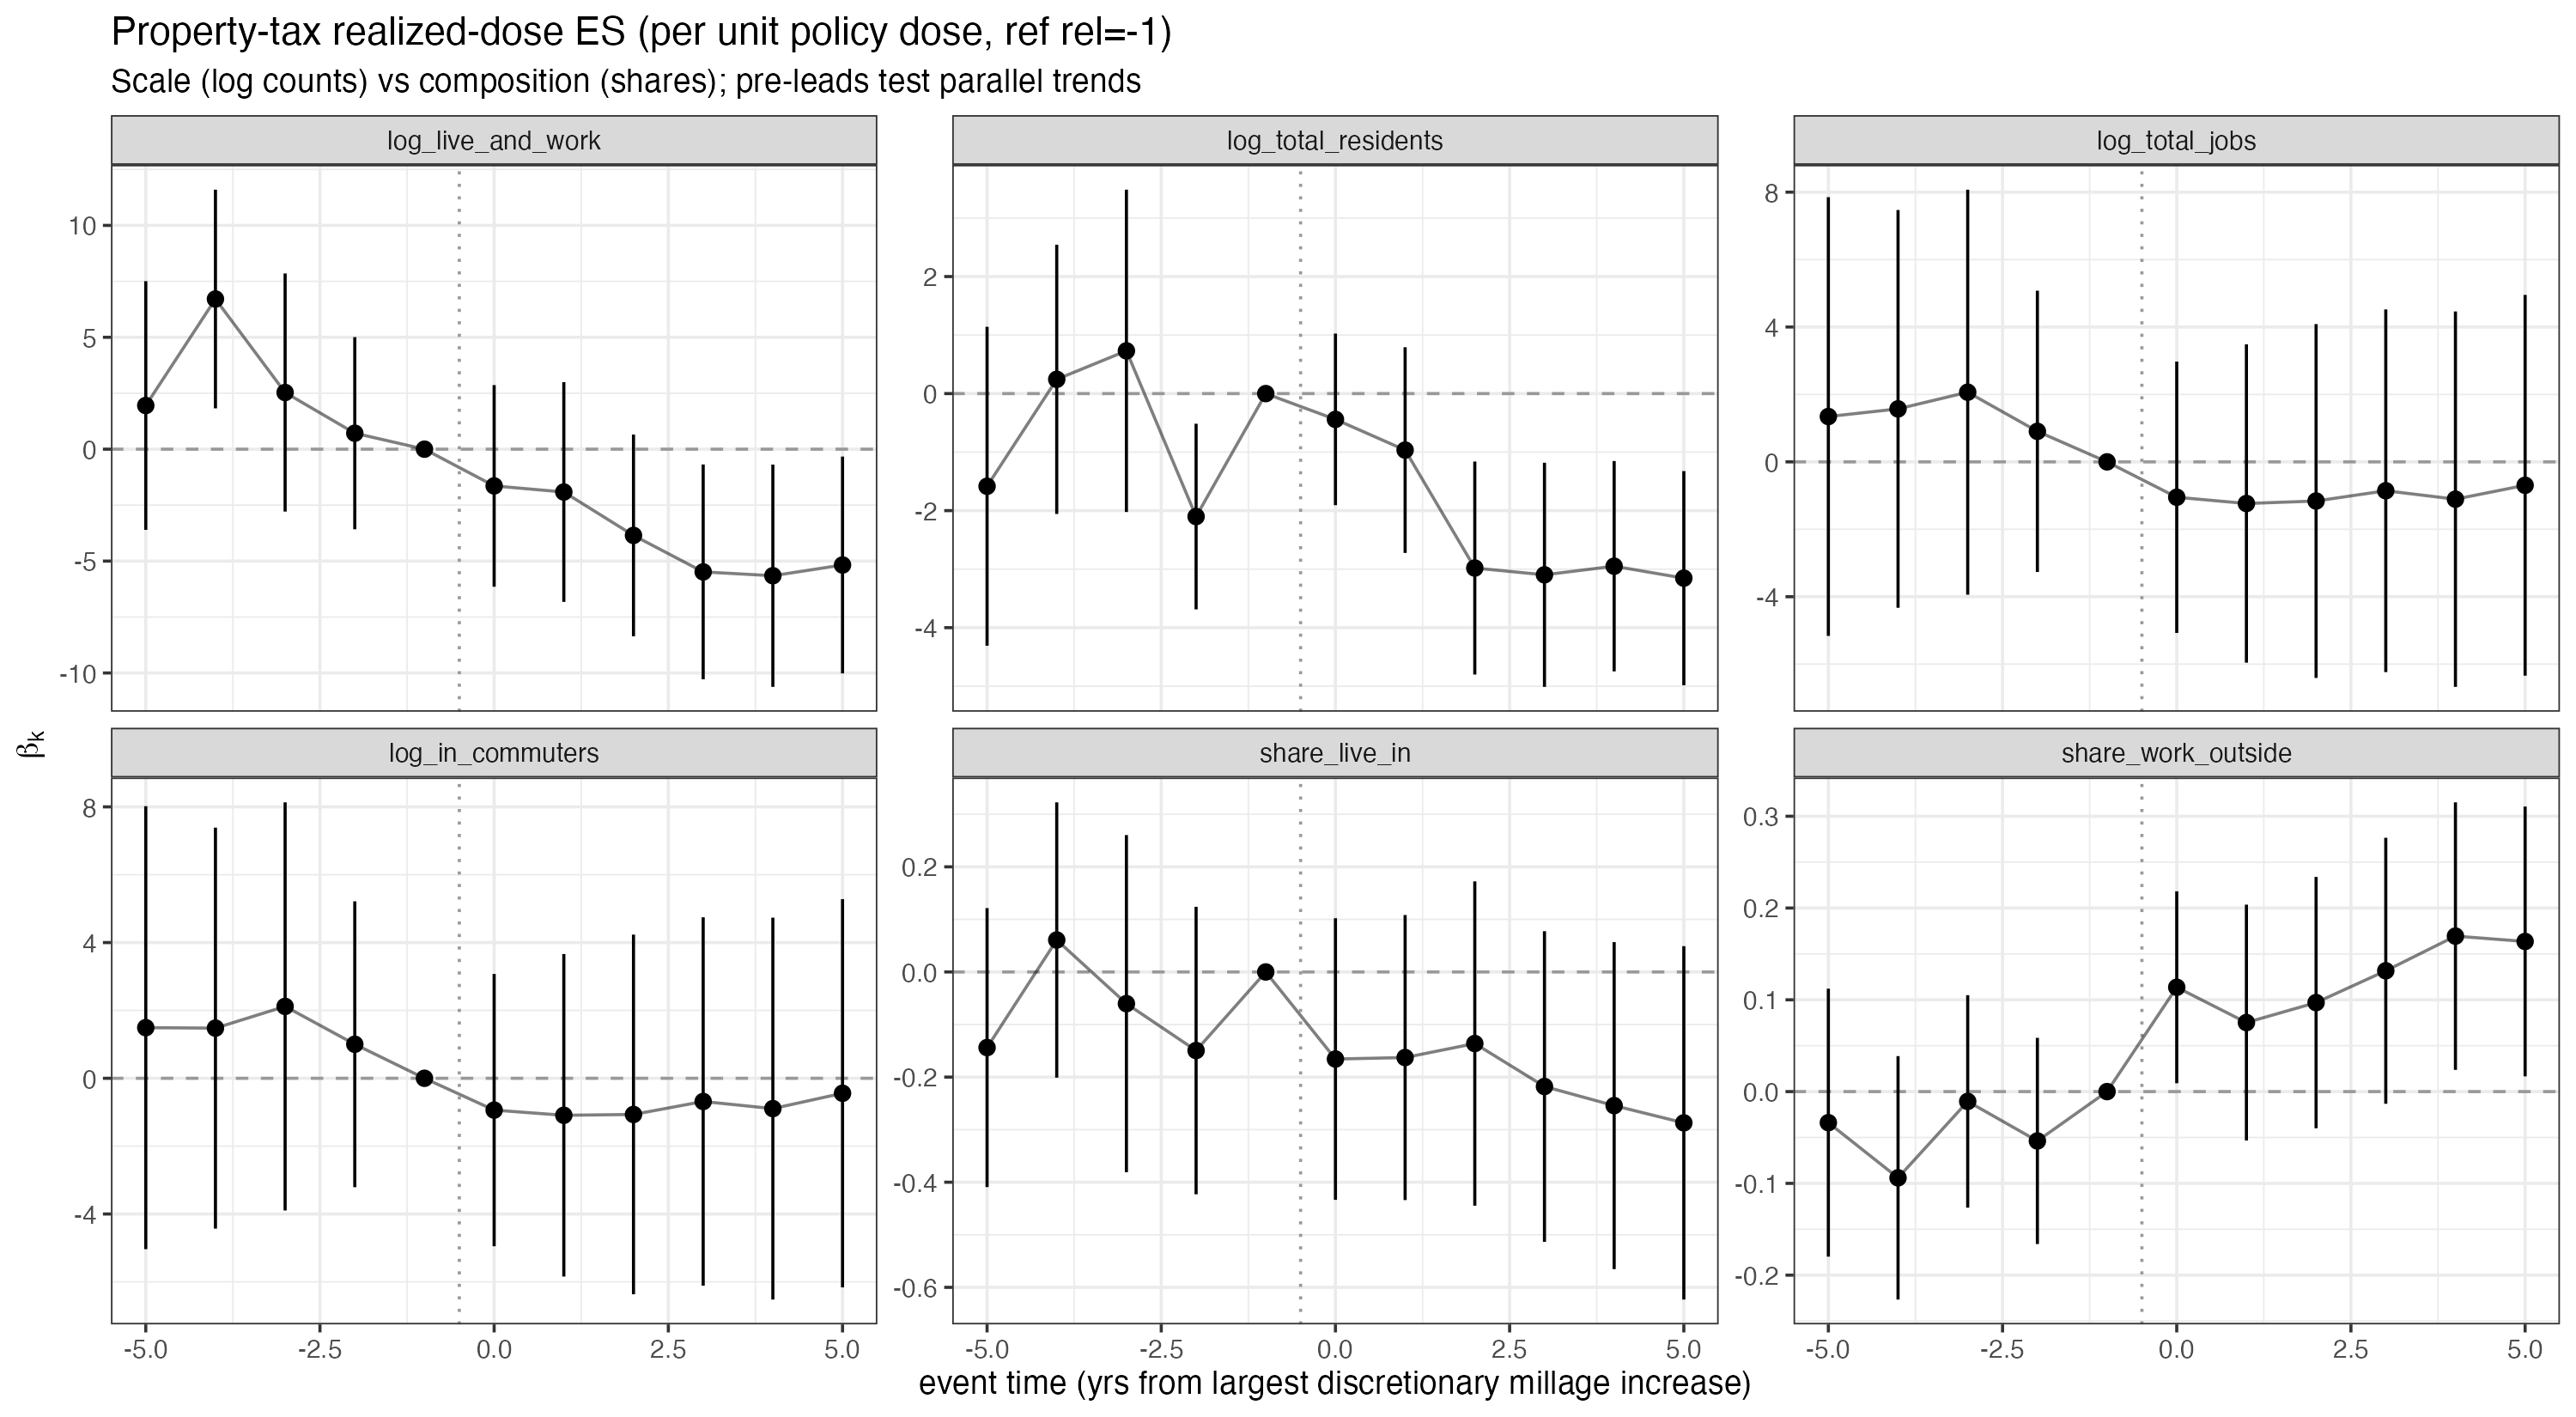
\includegraphics[width=0.95\textwidth]{../figures/proptax_es_scale_vs_comp.png}
  \begin{minipage}{0.95\textwidth}
    \footnotesize \textit{Notes:} Per-unit-of-policy-dose coefficient at
    each event time, faceted by outcome. The composition share and
    workplace counts have flat pre-trends; the residence counts pre-trend,
    so they are reported as honest-DiD bounds rather than point estimates.
  \end{minipage}
\end{figure}

%==========================================================
\subsection{Income versus Property Tax on a Common Dollar Basis}
\label{subsec:results-compare}

The income and property taxes are not directly comparable per percentage
point: one pp of EIT falls on earned income, one pp of effective property
rate on market value. I place them on a common basis---the percent change
in the outcome per \$1{,}000 of annual tax bill---using each
municipality's own median income and home value, so the comparison
reflects the actual cross-municipality distribution rather than two
representative constants. On every cleanly identified margin the
property-tax response is bounded an order of magnitude below the EIT, and
the property confidence interval excludes the EIT effect. Per \$1{,}000,
the EIT moves the local-employment count by $-0.99$ (log total jobs)
against a property-tax estimate of $-0.017$ with a $95\%$ interval of
$[-0.056, +0.023]$---a ratio of about $60\times$, with a sensitivity band
of roughly $43$--$82\times$ from the 10th--90th percentile of the
cross-municipality home-to-income ratio; the in-commuter and composition
margins give $53\times$ and $113\times$. Even the contaminated
residence-count margin, under the honest bounds, lies an order of
magnitude below the EIT's $-1.16$ per \$1{,}000. Residents respond to a
dollar of income tax roughly an order of magnitude---fifty to a hundred
times---more than to a dollar of property tax.

%==========================================================
\subsection{EIT Revenue Response}
\label{subsec:results-revenue}

Sorting erodes the tax base, so the revenue raised by a rate increase is
less than the mechanical projection. Estimating the same binding
decomposition with log EIT revenue as the outcome, a binding (Inc-bind)
increase raises EIT revenue with a net per-pp coefficient of $1.06$
($p<0.001$): revenue rises, but by less than a naive base-times-rate
projection. Splitting the cell by pre-event rate level, the
standard-structure (low-baseline) municipalities show a behavioral offset
of about $36\%$---roughly a third of the mechanically projected revenue
gain is offset by the base response---while the five high-baseline,
Home-Rule-heavy municipalities are not separately identified
($\beta=0.10$, $p=0.12$). This is a within-PA local-displacement offset on
the $24$-municipality Inc-bind cohort, not a state-level fiscal multiplier,
and it is the revenue counterpart of the sorting estimate: the same
movement of workers that shows up as the $-13\%$ live-and-work response
shows up here as a third of the projected revenue not materializing.

%==========================================================
\subsection{Summary}
\label{subsec:results-summary}

The headline finding is from the muni-level binding decomposition:
a 1 pp Inc-bind resident-rate increase reduces log live-and-work
by $-0.573^{***}$ with a clean realized-dose pre-trend
($p=0.33$) and a null Inc-nobind within-design placebo
($-0.073$). The same scaling on log in-commuters
gives $-0.412^{***}$. The pooled Inc benchmark in
Section~\ref{subsec:results-pooled} averages binding and
non-binding events, attenuating the Inc-bind effect to
$-0.287^{***}$, and the decomposition recovers the binding-channel
response. Full
coefficient tables with fiscal controls are in the appendix.

The property tax, estimated on the same municipalities with the
policy-driven effective-rate dose, shows no detectable sorting on the
cleanly identified margins (composition share and workplace counts) and
honest-DiD bounds that rule out an EIT-sized effect on the contaminated
residence-count margin. On a common per-\$1{,}000-of-annual-tax basis the
income tax moves residents roughly fifty to a hundred times more than
the property tax, a pattern consistent with the property burden
capitalizing into house prices rather than relocating households. The
revenue counterpart of the Inc-bind sorting response is a behavioral
offset of about a third of the mechanically projected revenue gain for
standard-structure municipalities.

\section{Robustness}
\label{sec:robustness}
%==========================================================

This section summarizes the robustness checks behind the headline
muni-level dose-response. The realized-dose event-study pre-trend
diagnostic was discussed alongside the headline in
Section~\ref{subsubsec:decomp-es}. Full tables behind the
robustness summaries are in Appendix~\ref{app:robustness}.

\subsection{Pre/Post Act 32 Decomposition}
\label{subsec:rob-act32}

Splitting the headline cell-$\times$-dose specification at the Act-32
enforcement break (cohort first event year $<2012$ vs $\geq 2012$)
shows the municipality-level binding-cell effect strengthens after
consolidated employer withholding takes effect ($-0.593^{**}$ pre vs
$-0.546^{***}$ post on log residents working in own municipality)
(\hyperref[app:rob-act32]{see Appendix~\ref{app:rob-act32}}).

\subsection{Act 47 Distressed-Municipality Exclusion}
\label{subsec:rob-act47}

The Inc-bind cohort includes Act~47 distressed cities
\citep{paAct47_1987}. Act~47 is the legal designation that
lets a municipality exceed the $0.5\%$ statutory municipality-EIT
cap meaning there may be a selection confounder. An
Act~47 designation may come from a period of population
decline, (rate hike occurs after the municipality is
already losing residents), debt
restructuring, and service cuts. Only
$2$ of the $24$ Inc-bind municipalities match the DCED Act~47
designation list (Carbondale and Hazleton). The other historically
Act-47-designated PA cities (e.g.\ Braddock, Coatesville, Johnstown)
do not appear in the Inc-bind cell here because their rate trajectories are non-monotone (did not move in one direction) and were removed (Section~\ref{subsec:stacked-continuous}).
Table~\ref{tab:act47_robustness} re-estimates the
municipality-level Inc-bind coefficient on the remaining $22$
non-Act-47 Inc-bind municipalities.

\begin{table}[H]
  \centering
  \caption{Act~47 robustness: dropping distressed Inc-bind municipalities from the cousub headline}
  \label{tab:act47_robustness}
  \small
  \begin{tabular}{lcc}
    \toprule
    Outcome & All 24 Inc-bind & Drop 2 Act~47 \\
    \midrule
    log live-and-work & $-0.718^{***}$ (0.214) & $-0.482^{**}$ (0.191) \\
    log in-commuters & $-0.540^{***}$ (0.165) & $-0.419^{**}$ (0.172) \\
    log total jobs & $-0.621^{***}$ (0.172) & $-0.462^{***}$ (0.167) \\
    live-in-muni share & $-0.059^{***}$ (0.020) & $-0.034^{**}$ (0.015) \\
    \bottomrule
  \end{tabular}
  \vspace{0.3em}
  \begin{minipage}{0.85\textwidth}
    \footnotesize \textit{Notes:} Muni-level Inc-bind coefficient on each residence-side outcome, with same FE / cluster / controls as the headline. Column 1 is the headline (all 24 Inc-bind municipalities). Column 2 drops 2 Act 47 distressed-designation municipalities from the Inc-bind cohort; the remaining 22 Inc-bind municipalities are mostly Home Rule and Boroughs. Cluster-robust SEs in parentheses. $^{*}p<0.10$, $^{**}p<0.05$, $^{***}p<0.01$.
  \end{minipage}
\end{table}



The point estimates are direction-preserving and modestly smaller
when the two Act~47 munis are dropped. The live-and-work
coefficient moves from $-0.72$ to $-0.48$, in-commuters from
$-0.54$ to $-0.42$, total jobs from $-0.62$ to $-0.46$, and the
live-in-muni share from $-0.059$ to $-0.034$. All four coefficients
remain statistically significant at $5\%$ or better on the trimmed
sample, so the headline is not purely driven by Act~47 selection. The
attenuation when Act~47 cities are removed is consistent with those
two cities having larger doses.

\subsection{Property-Tax Treatment and Honest-DiD Sensitivity}
\label{subsec:rob-proptax}

Two checks bound the property-tax conclusion. First, the no-detectable-
sorting result on the clean margins is unchanged whether the treatment
is the policy-only dose (discretionary millage valued at the baseline
assessment ratio, the headline) or the realized effective-rate dose
(millage $\times$ contemporaneous CLR): the latter carries the endogenous
assessment drift and is reported only as a robustness check, and the
clean-margin coefficients remain small and statistically insignificant
under both. Second, on the contaminated residence-count margins I report
Rambachan--Roth bounds across relative-magnitude budgets; at $\bar M=1$
the bounds include zero (the residence response is not separately
identified) while still excluding the EIT-sized per-dollar effect, and
they widen monotonically with $\bar M$. The property-tax result is thus
robust in the only senses available to it: it does not depend on the
dose construction, and its honest bounds rule out an income-tax-scale
response without claiming a clean zero.

%==========================================================
\section{Discussion}
\label{sec:discussion}
%==========================================================

The main finding of this paper is that sorting is identified through the
binding mechanism. The Inc-bind realized dose of
$0.24$ pp cumulative over five years, the municipal resident-rate
increase reduces the log count of workers who both live and work in
the municipality by roughly $13\%$. The Inc-nobind
placebo is not statistically significant, and Inc-becomes
lies between the two with a smaller statistically significant effects. The pattern matches the mechanism
prediction. The same statutory rate change can produce a strong,
moderate, or null behavioral response depending solely on whether
the rate moves the worker's bill. This is direct evidence that
workers respond to taxes they actually pay rather than to statutory
rates per se. The per-pp coefficient ($-0.573$, or about $44\%$ per
pp) is the regression slope and should not be read as a
typical-event magnitude. A $1$ pp shock is quite far above the median realized dose in this cohort.

Identification at the municipality level is supported by the
realized-dose pre-trend diagnostic. The joint Wald test on the Inc-bind cell does not reject parallel
trends ($p = 0.33$). The 24-municipality Inc-bind cohort identifies a causal effect, but generally eastern-PA-concentrated
set of Home Rule boroughs and Act~47 designees.

Other outcome variables suggest a general decline in economies of these cites such as the in-commuters coefficient is also negative
($-0.412^{\ast\ast\ast}$). If
residents only relocated their home while keeping their
job in the rate-raising municipalities, in-commuters would
theoretically rise as someone has to fill the displaced residents' jobs. If Inc-bind munis
were raising the work rate $\tau^{\text{work,M}}$ at the same time
as the resident rate, in-commuters would mechanically face a higher
withholding bill on their own paychecks and the negative coefficient
would have a direct work-side explanation. The data does not support that explanation. At the first-event year municipalities raise
only the resident rate and leave the work rate unchanged. The negative
in-commuters coefficient therefore reflects a broader local
labor-market response to municipal fiscal stress, when the binding home-side rate rises rather than a
mechanical tax on in-commuters' bills.

The models also incorporate the two-rate-setting mechanisms (municipality and school distircts). The municipality resident-rate Inc-bind
coefficient is large and negative, while the SD resident-rate
coefficient in the same joint regression is small and
positive, but not statistically significant. In the aggregate model the SD rate increases are associated with increased sorting within those cities. Although the models are mixed on statistical significance, the evidence is suggestive of the tax-amenity-bundle model. SD
revenues primarily fund schools, which may be viewed as high quality schools thus capitalizing into the
willingness to pay to reside in the district. The municipal resident-rate may be less salient to workers as the revenue funds streets, debt service,
intergovernmental transfers, and general administration.
The sign contrast is suggestive evidence of bundle-level Tiebout
sorting and strengthens the binding-channel interpretation rather
than complicating it. The binding rule tells us which rate
events move workers' bills, and the rate-setter contrast tells us
how workers value the revenue once collected.

Six limitations merit acknowledgment. First, the LODES OD data
covers PA municipalities but not cross-state inflows in the
intra-state main file used here. Incorporating this data would
tighten the estimates of in-commuters for border municipalities.

Second, the paper estimates the residential-sorting response to the
home-side resident rate but does not separately estimate the
work-side response to the municipality work rate ($\tau^{\text{work,muni}}$).
The work rate enters the design only through the
binding classification of cells. A complementary work-side
specification---estimating in-commuter and total-jobs responses to
$\tau^{\text{work,muni}}$ events at the municipality level, with a parallel
binding decomposition, testing the work side of the mechanism. I defer this to future work.

Third, the per-pp coefficient is a displacement elasticity. The Inc-bind cohort is concentrated in eastern PA
(Figure~\ref{fig:pa_map}). A worker leaving municipality (A) for an
adjacent municipality (B) shows up as a $-1$ in municipality (A) live-and-work
count and a $+1$ to that neighbor's residence count. The
headline specification partially absorbs neighbor-rate variation
through never-changed-only controls and municipality-by-stack
fixed effects, but it does not formally model spatial spillovers,
and a worker moving to an adjacent municipality whose rate is also moving
violates SUTVA. The
\citet{buttsDifferenceinDifferencesEstimationSpatial2023}
estimator would permit me to generalize the stacked DiD to allow for SUTVA violations
from spatial spillovers across treated units, using an explicit
spatial weighting matrix. Applying this is left for future work.

Fourth, LODES is a stock dataset rather than a person-linked
flow dataset. For each (residence municipality, workplace municipality, year), I
observe a count of workers, not individual migration flows. The headline coefficient on the municipality count of residents
is therefore a net elasticity as measured by the difference of gross outflows and inflows. The paper's evidence that municipal rate
hikes reduce the residential count is consistent both with workers
leaving and with workers not arriving to replace those who left, however,
LODES alone cannot decompose the two. Decomposing into gross
outflow and gross inflow would require person-linked
administrative data: the IRS Statistics of Income individual master
file, the American Community Survey microdata with full
residence-history linkage, or the LEHD
Job-to-Job Flows file, which tracks the same workers across
employer transitions at quarterly frequency. All three are
restricted-access products requiring approved-project status under
the Census Bureau's Federal Statistical Research Data Centers
(FSRDCs) or IRS Statistics of Income agreements. The microdata
cannot be exported and must be analyzed at a physical FSRDC
location. Replicating the present analysis on person-linked data
is a clear extension but not currently being undertaken at this time.

The comparison with the property tax sharpens the interpretation. Per
dollar of annual tax, residents respond to the income tax roughly an
order of magnitude more than to the property tax, and on the cleanly
identified margins the property-tax response is statistically
indistinguishable from zero. This is what the capitalization view
predicts \citep{oates1969}: a property-tax increase is substantially
absorbed into lower house prices, so the burden reaching a mobile
household is smaller than the statutory change and is borne in part by
the immobile asset rather than the person, while an income-tax increase
falls on the mobile earner directly. I read the pattern as consistent
with capitalization rather than as proof of it, because I do not observe
the house-price response that capitalization implies; what the data
establish is that the property tax causes far less sorting per dollar
than the income tax, not the channel through which the response is muted.

The two legs are deliberately not identified equally well, and the
asymmetry is informative rather than a shortcoming. The EIT's piecewise
rule makes its design self-falsifying through the Inc-nobind placebo; the
property tax, a continuous treatment with no never-treated group and no
placebo, rests on its realized-dose pre-trend alone. That single check
passes on the composition and workplace margins and fails on the
residence-count margins, where municipalities raising the property tax
are already on diverging resident trajectories, so I report those margins
as honest-DiD bounds rather than point estimates. Two caveats bound the
comparison. Its magnitude rests on the EIT binding-cell estimate, which
is large; under any reasonable discount of it the property-tax response
remains far smaller. And the residence-count margin is an
\emph{unidentified} null, not a clean one: the honest bounds rule out an
EIT-sized effect but include zero.

%==========================================================
\section{Conclusion}
\label{sec:conclusion}
%==========================================================

This paper answers the question, when do local income taxes cause residential sorting? In
Pennsylvania, when the piecewise max-rule makes a statutory rate
increase it can mechanically change the worker's tax bill. Under the Inc-bind cell, the
increase reduces the count of workers who both live and work in
their own municipality by roughly $13\%$
with clean realized-dose pre-trends, and a
null finding in the Inc-nobind placebo. This is a local effect for a small
cohort of binding rate-raisers rather than a state-average
elasticity.

The design delivers the within-design heterogeneity that
\citet{agrawalLessonsStateLocal} finds missing from the US
local-income-tax literature. The piecewise rule splits
otherwise-identical rate increases into cells that moves the
worker's bill (Inc-bind) and a placebo cell that does not
(Inc-nobind), making the design self-falsifying in a way that
pooled local-tax regressions cannot. The municipality and schoold district estimations are opposite with a negative results on the municipality rate and positive on the SD rate. This is
consistent with workers sorting on the bundle of taxes and
amenities rather than on rates alone.


The natural next step is a companion paper on the work-side
response to the muni work rate $\tau^{\text{work,muni}}$, which
enters the present design only through the binding classification
of cells. More broadly, the framework is portable to any setting
where a piecewise tax rule determines whether a statutory change
reaches the taxpayer's bill, such as local income taxes and property taxes.

% \section*{Acknowledgments}
% TODO: fill in before submission

%==========================================================
% BIBLIOGRAPHY
%==========================================================
\printbibliography

%==========================================================
% APPENDIX
%==========================================================
\appendix

%==========================================================
\section{Full Results with Control Coefficients}
\label{app:full-results}
%==========================================================

This appendix reports the muni-level binding-decomposition
regression with the fiscal-control coefficients and diagnostics.
Table~\ref{tab:app_full_muni_cell_results} reports the muni-rate
and SD-rate cells (two panels) with the shared fiscal controls from
the same joint regression.

\begin{table}[!htbp]
  \centering
  \caption{Municipality-level dose-response: muni resident-rate cells with fiscal controls (full spec)}
  \label{tab:app_full_muni_cell_results}
  \footnotesize
  \renewcommand{\arraystretch}{0.9}
  \resizebox{\textwidth}{!}{
  \begin{tabular}{lcccc}
    \toprule
    Outcome & Log(work in own muni) & Log(in-commuters) & Log(employed residents) & Share live in muni \\
    \midrule
    \textbf{Inc-bind} & -0.573\sym{***} & -0.421\sym{***} & -0.104\sym{**} & -0.057\sym{***} \\
                      & (0.162) & (0.126) & (0.043) & (0.020) \\
    \textbf{Inc-becomes} & -0.239\sym{***} & -0.247\sym{***} & -0.040 & -0.012 \\
                      & (0.055) & (0.055) & (0.026) & (0.011) \\
    \textbf{Inc-nobind} & -0.082 & -0.657 & 0.235\sym{***} & -0.015 \\
                      & (0.143) & (0.653) & (0.077) & (0.027) \\
    \textbf{Dec-bind} & 0.222\sym{*} & 0.152 & 0.077 & 0.010\sym{***} \\
                      & (0.114) & (0.107) & (0.138) & (0.002) \\
    \textbf{Dec-becomes-non} & -1.221\sym{***} & 0.184\sym{**} & -1.482\sym{***} & -0.146\sym{***} \\
                      & (0.071) & (0.072) & (0.033) & (0.005) \\
    \textbf{Dec-nobind} & --- & 0.150\sym{***} & -0.228\sym{***} & 0.013\sym{***} \\
                      &  & (0.010) & (0.005) & (0.001) \\
    \midrule
    \multicolumn{5}{l}{\textit{Fiscal controls}} \\
    police-services share & 0.104 & -0.015 & 0.005 & 0.008 \\
                      & (0.100) & (0.104) & (0.058) & (0.007) \\
    streets share & 0.051 & 0.006 & -0.001 & 0.002 \\
                      & (0.040) & (0.040) & (0.019) & (0.003) \\
    debt-service share & -0.052 & -0.021 & 0.018 & 0.004 \\
                      & (0.051) & (0.058) & (0.029) & (0.005) \\
    EIT-revenue share & -0.024 & 0.261\sym{***} & 0.017 & -0.013\sym{*} \\
                      & (0.086) & (0.084) & (0.041) & (0.007) \\
    real-estate-tax share & -0.180\sym{**} & -0.263\sym{***} & -0.040 & -0.008 \\
                      & (0.087) & (0.094) & (0.041) & (0.007) \\
    intergovernmental-revenue share & 0.027 & 0.036 & 0.067\sym{***} & 0.005 \\
                      & (0.044) & (0.048) & (0.023) & (0.004) \\
    \midrule
    $N$ & 193,699 & 211,780 & 215,159 & 211,789 \\
    $R^2$ & 0.964 & 0.960 & 0.981 & 0.825 \\
    Within $R^2$ & 0.001 & 0.001 & 0.001 & 0.001 \\
    Dep.\ mean & 3.663 & 5.839 & 6.688 & 0.093 \\
    Dep.\ SD & 1.920 & 1.878 & 1.294 & 0.075 \\
    \bottomrule
  \end{tabular}
  }
  \vspace{0.3em}
  \begin{minipage}{0.95\textwidth}
    \footnotesize \textit{Notes:} Stacked-DiD; muni$\times$stack and year$\times$stack FE; SE clustered at muni. SE in parens. $^{*}p<0.10$, $^{**}p<0.05$, $^{***}p<0.01$.
  \end{minipage}
\end{table}


%==========================================================
\section{Realized-Dose Event Studies, Full Set}
\label{app:es-realized}
%==========================================================

Per-cell realized-dose Sun--Abraham event studies at the muni
level for the remaining residence-side outcomes (log live-and-work
is in the body, \S\ref{subsubsec:decomp-es}).

\begin{figure}[H]
  \centering
  \caption{Muni-level realized-dose ES on $\log(\text{in-commuters})$, by cell.}
  \label{fig:app_es_realized_muni_incomm}
  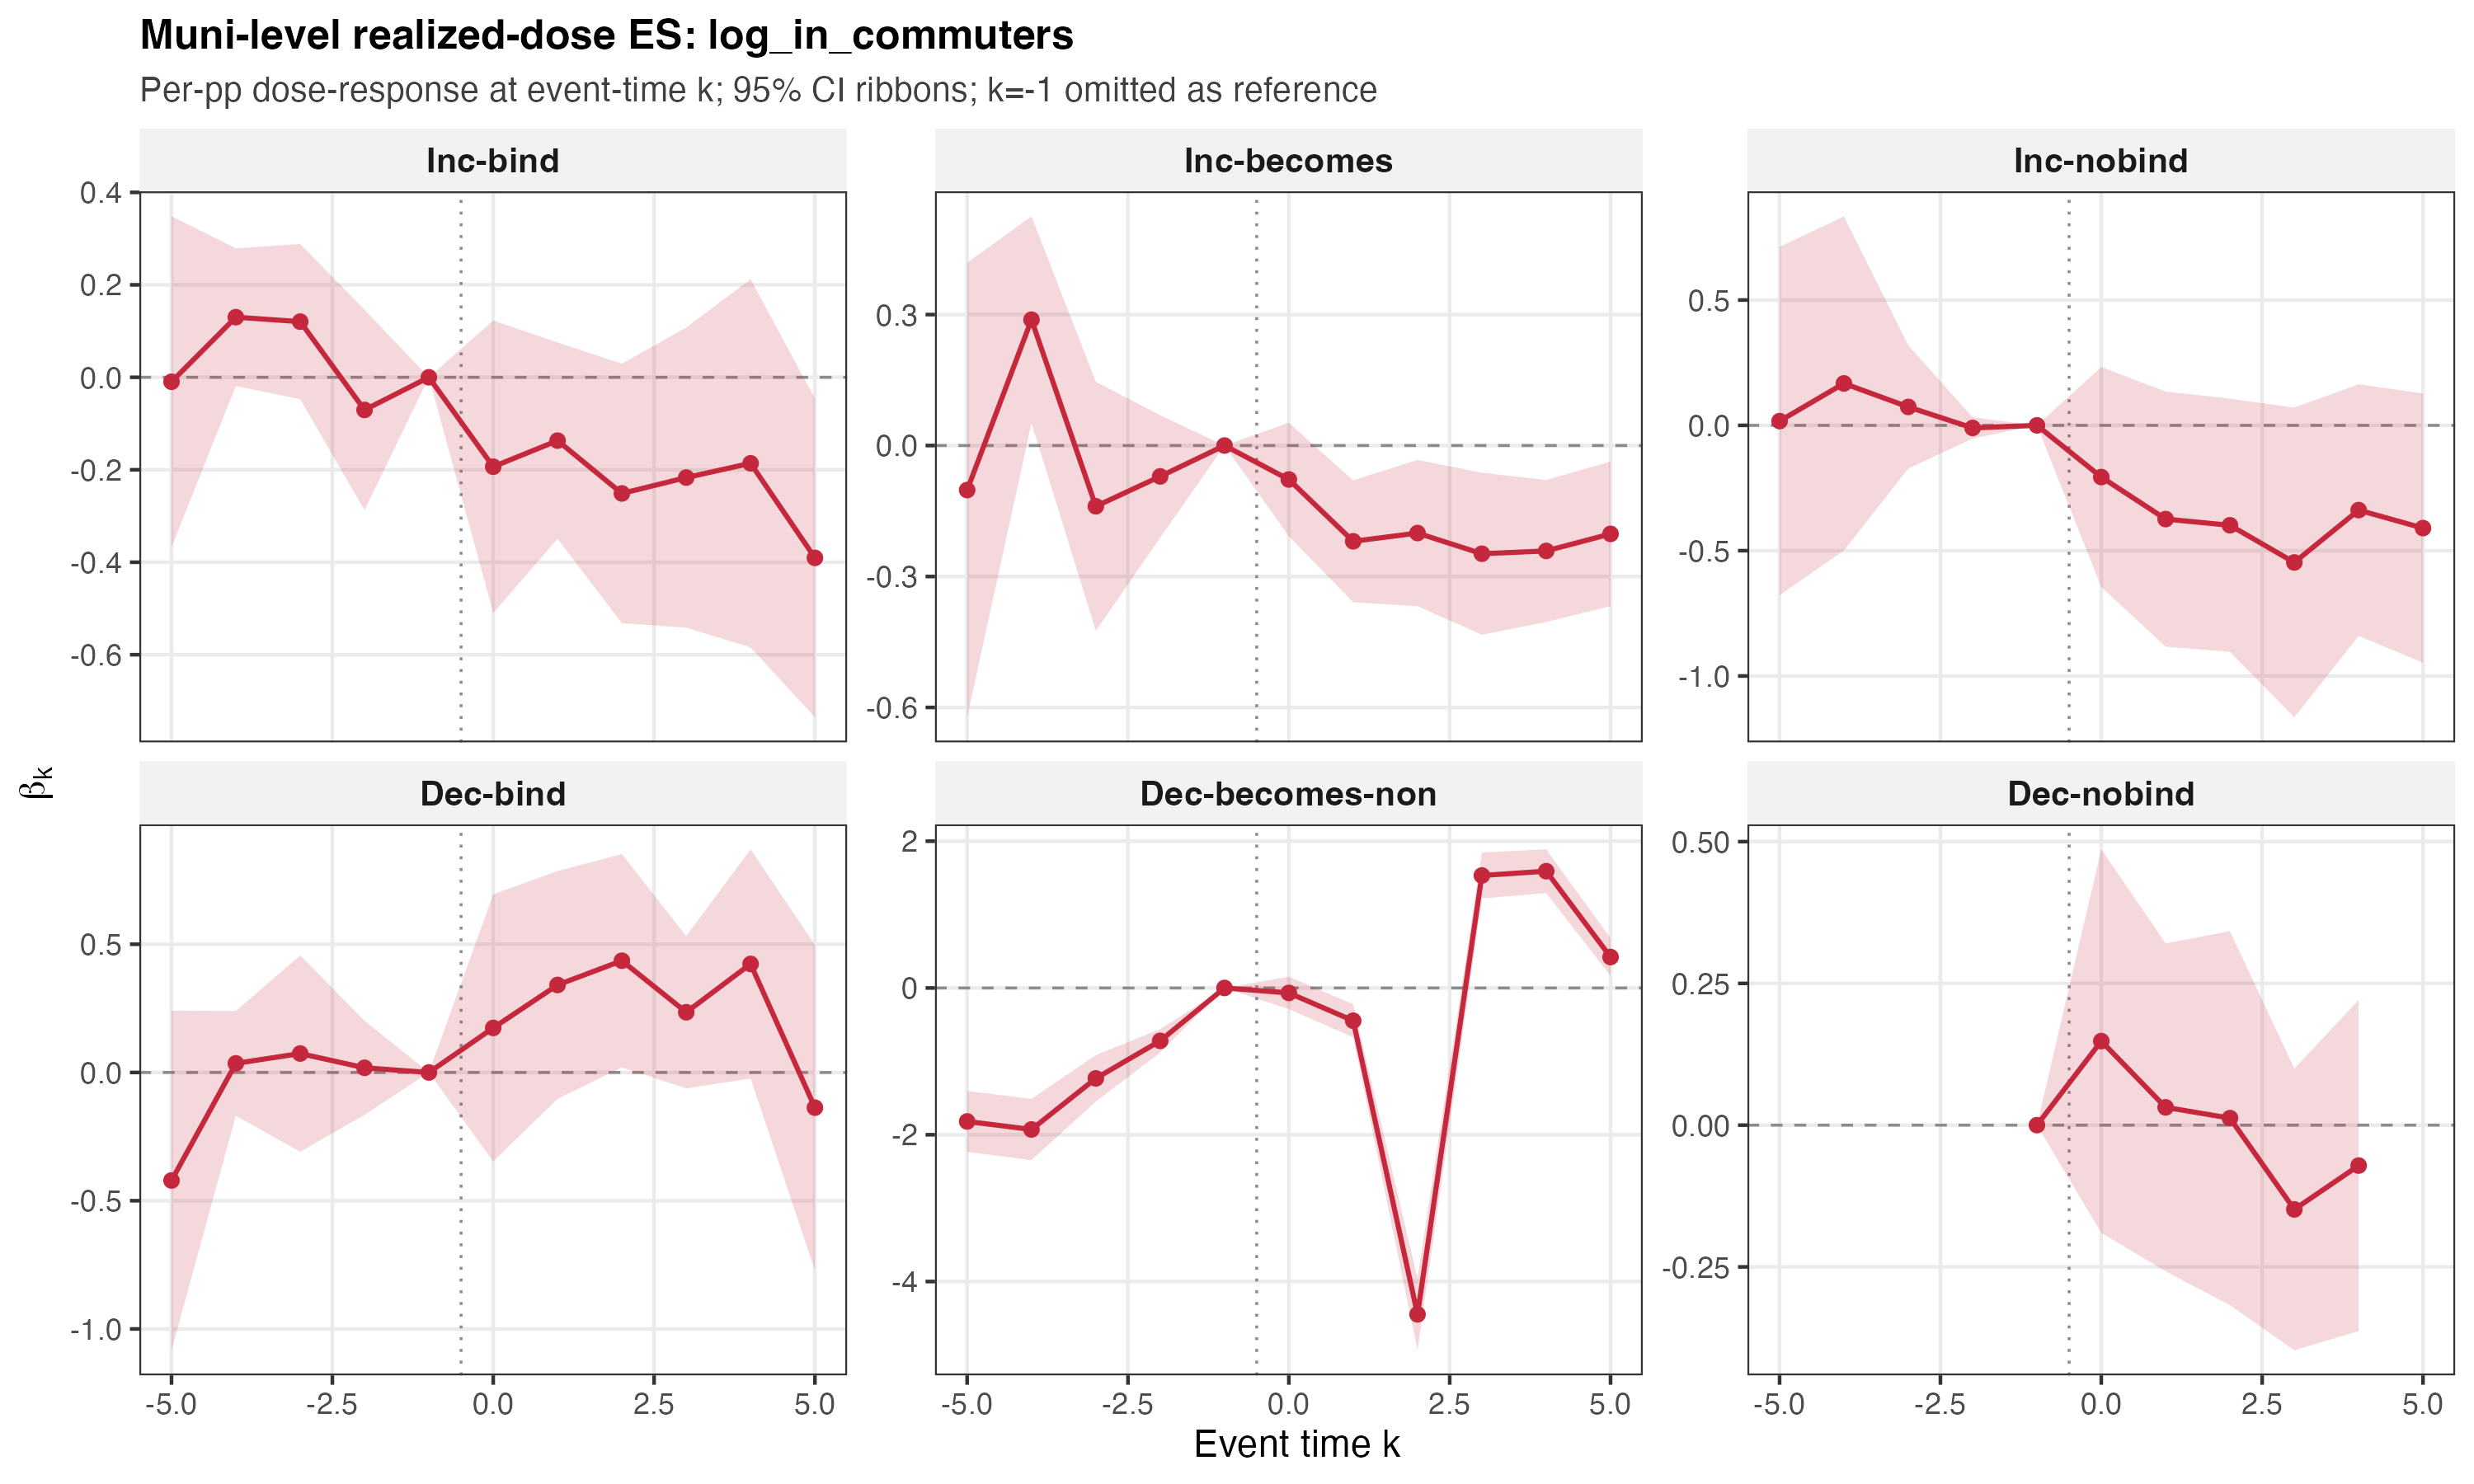
\includegraphics[width=0.95\textwidth]{../figures/es_realized_log_in_commuters.png}
\end{figure}

\begin{figure}[H]
  \centering
  \caption{Muni-level realized-dose ES on $\log(\text{total jobs})$, by cell.}
  \label{fig:app_es_realized_muni_jobs}
  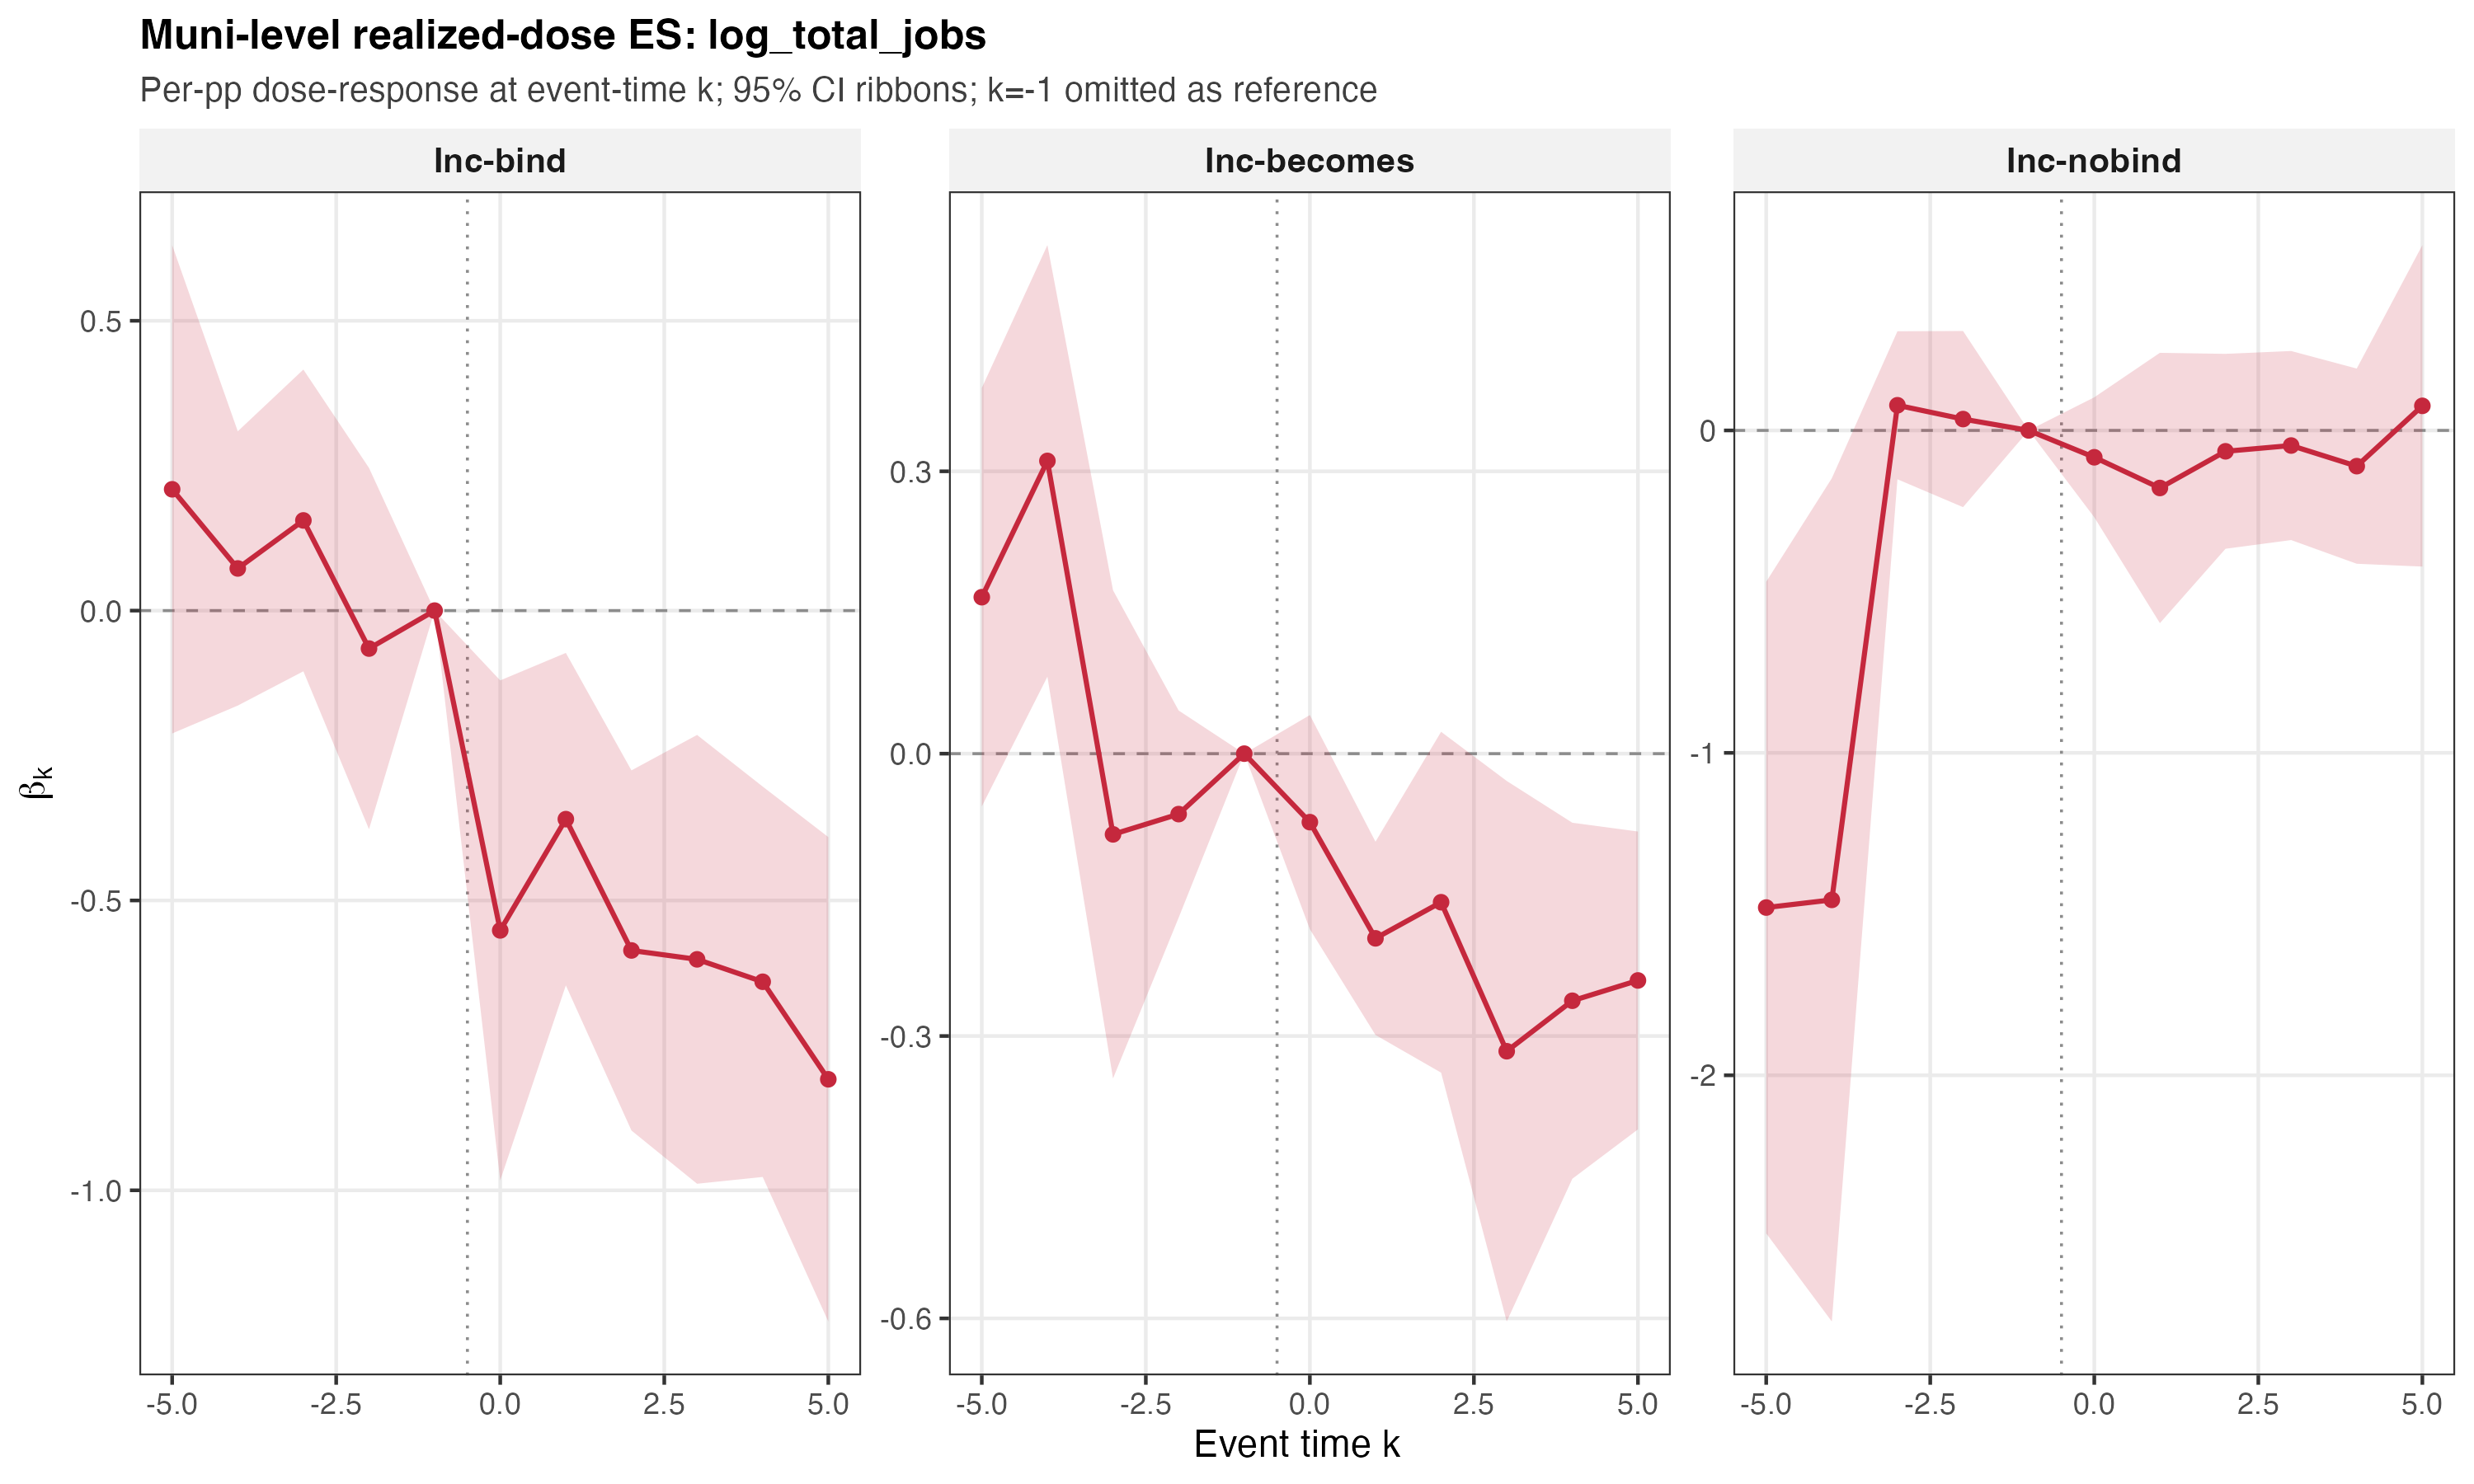
\includegraphics[width=0.95\textwidth]{../figures/es_realized_log_total_jobs.png}
\end{figure}

\begin{figure}[H]
  \centering
  \caption{Muni-level realized-dose ES on the share of workers
           living in their own municipality, by cell.}
  \label{fig:app_es_realized_muni_share_in}
  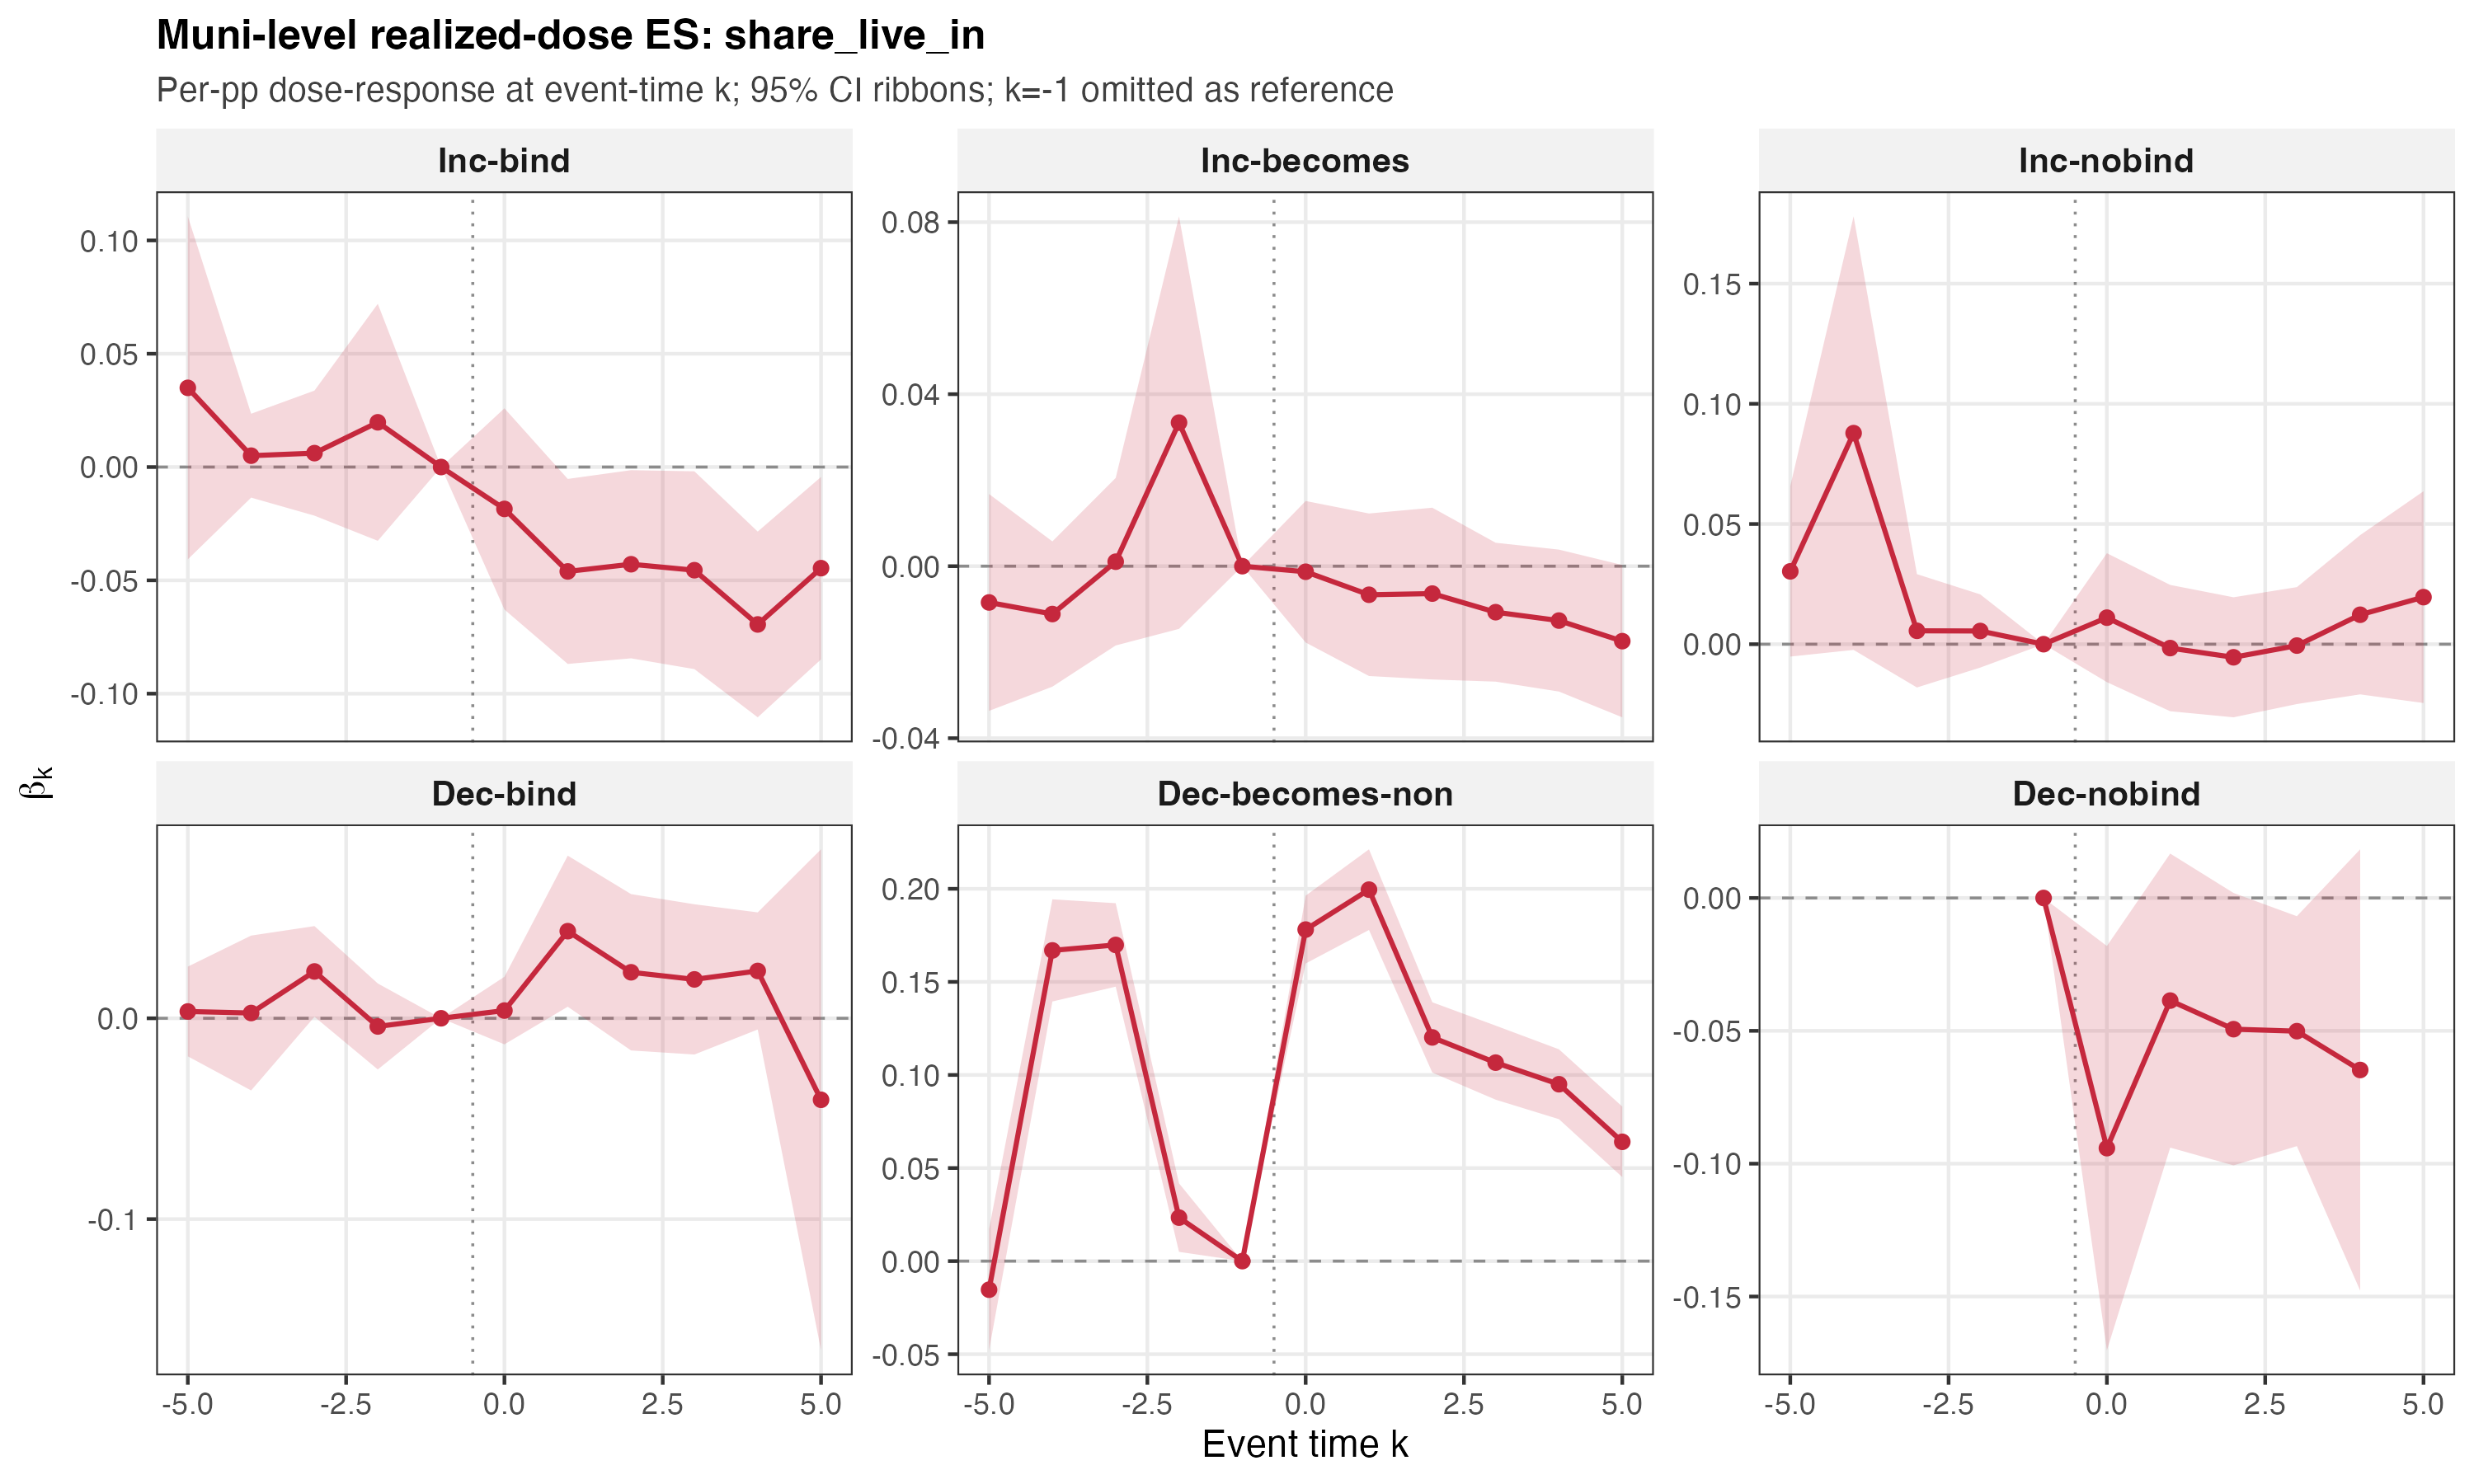
\includegraphics[width=0.95\textwidth]{../figures/es_realized_share_live_in.png}
\end{figure}

%==========================================================
\section{Robustness: Full Tables}
\label{app:robustness}
%==========================================================

Full tables behind the robustness summaries in
Section~\ref{sec:robustness}.

\subsection{Pre/post Act 32 split}
\label{app:rob-act32}

Headline cell $\times$ dose specification re-estimated on pre-Act-32
($c<2012$) and post-Act-32 ($c\geq 2012$) cohort subsamples at the
municipality level.

\begin{table}[H]
  \centering
  \caption{Pre-/post-Act-32 split --- municipality level}
  \label{tab:act32_cousub}
  \small
  \resizebox{\textwidth}{!}{
  \begin{tabular}{lcccc}
    \toprule
    Outcome & Log(work in own muni) & Log(in-commuters) & Log(employed residents) & Share live in muni \\
    \midrule
    \textbf{Inc-bind} & & & & \\
    \quad Pre-Act 32 & -0.339\sym{**} & -0.156 & -0.098\sym{**} & -0.047\sym{***} \\
                    & (0.138) & (0.112) & (0.045) & (0.013) \\
    \quad Post-Act 32 & -0.534\sym{***} & -0.334\sym{***} & -0.104\sym{***} & -0.040\sym{***} \\
                    & (0.075) & (0.080) & (0.034) & (0.004) \\
    \textbf{Inc-becomes} & & & & \\
    \quad Pre-Act 32 & -0.230\sym{**} & -0.239\sym{***} & -0.131\sym{*} & -0.029\sym{*} \\
                    & (0.093) & (0.089) & (0.074) & (0.016) \\
    \quad Post-Act 32 & -0.143 & -0.160 & -0.013 & 0.003 \\
                    & (0.106) & (0.108) & (0.019) & (0.009) \\
    \textbf{Inc-nobind} & & & & \\
    \quad Pre-Act 32 & -0.051 & -0.078 & -0.052\sym{**} & -0.013 \\
                    & (0.220) & (0.157) & (0.026) & (0.010) \\
    \quad Post-Act 32 & -0.094 & -0.305 & 0.365\sym{***} & -0.010 \\
                    & (0.113) & (0.368) & (0.095) & (0.013) \\
    \textbf{Dec-bind} & & & & \\
    \quad Pre-Act 32 & 0.341\sym{***} & 0.049 & -0.013 & 0.074\sym{*} \\
                    & (0.046) & (0.135) & (0.277) & (0.044) \\
    \quad Post-Act 32 & 0.068 & 0.056 & -0.133 & 0.008\sym{***} \\
                    & (0.144) & (0.183) & (0.102) & (0.003) \\
    \textbf{Dec-becomes-non} & & & & \\
    \quad Pre-Act 32 & -1.220\sym{***} & 0.177\sym{**} & -1.474\sym{***} & -0.144\sym{***} \\
                    & (0.069) & (0.071) & (0.032) & (0.005) \\
    \quad Post-Act 32 & 1.384\sym{***} & 0.874\sym{***} & 0.734\sym{***} & 0.057\sym{***} \\
                    & (0.106) & (0.112) & (0.053) & (0.008) \\
    \textbf{Dec-nobind} & & & & \\
    \quad Pre-Act 32 & 0.377\sym{***} & -0.211 & 0.397\sym{***} & 0.019 \\
                    & (0.106) & (0.218) & (0.018) & (0.047) \\
    \quad Post-Act 32 & 0.094\sym{***} & 0.177\sym{***} & -0.132 & 0.006 \\
                    & (0.019) & (0.027) & (0.090) & (0.006) \\
    \midrule
    \textit{Pre-Act 32} & & & & \\
    \quad $N$ & 218,438 & 238,760 & 242,447 & 238,770 \\
    \quad $R^2$ & 0.964 & 0.959 & 0.981 & 0.823 \\
    \quad Within $R^2$ & 0.001 & 0.001 & 0.001 & 0.001 \\
    \quad Dep.\ mean & 3.675 & 5.845 & 6.696 & 0.093 \\
    \quad Dep.\ SD & 1.933 & 1.886 & 1.298 & 0.075 \\
    \textit{Post-Act 32} & & & & \\
    \quad $N$ & 218,036 & 238,336 & 242,033 & 238,346 \\
    \quad $R^2$ & 0.964 & 0.959 & 0.981 & 0.823 \\
    \quad Within $R^2$ & 0.001 & 0.001 & 0.001 & 0.001 \\
    \quad Dep.\ mean & 3.672 & 5.843 & 6.695 & 0.093 \\
    \quad Dep.\ SD & 1.932 & 1.885 & 1.297 & 0.075 \\
    \bottomrule
  \end{tabular}
  }
  \vspace{0.3em}
  \begin{minipage}{0.95\textwidth}
    \footnotesize \textit{Notes:} Cluster-robust standard errors in parentheses. Treated cohorts split at first event year $c < 2012$ (Pre-Act~32) vs $c \geq 2012$ (Post-Act~32). At the muni level, the Inc-bind coefficient on log live-and-work strengthens from $-0.339^{**}$ (pre) to $-0.534^{***}$ (post), consistent with consolidated employer withholding making the EIT binding \citep{bagchiEffectsIntroducingWithholding2022}; the within-design placebo (Inc-nobind) is null in both periods. $^{*}p<0.10$, $^{**}p<0.05$, $^{***}p<0.01$.
  \end{minipage}
\end{table}


%==========================================================
\end{document}
